\documentclass[10pt]{article}
\usepackage[letterpaper]{geometry}
\geometry{verbose,tmargin=1in,bmargin=1in,lmargin=1in,rmargin=1in}
\usepackage{setspace}
\usepackage{ragged2e}
\usepackage{color}
\usepackage{titlesec}
\usepackage{graphicx}
\usepackage{float}
\usepackage{mathtools}
\usepackage{amsmath}
\usepackage[font=small,labelfont=bf,labelsep=period]{caption}
\usepackage[english]{babel}
\usepackage{indentfirst}
\usepackage{array}
\usepackage{makecell}
\usepackage[usenames,dvipsnames]{xcolor}
\usepackage{multirow}
\usepackage{tabularx}
\usepackage{arydshln}
\usepackage{caption}
\usepackage{subcaption}
\usepackage{xfrac}
\usepackage{etoolbox}
\usepackage{cite}
\usepackage{url}
\usepackage{dcolumn}
\usepackage{hyperref}
\usepackage{courier}
\usepackage{url}
\usepackage{esvect}
\usepackage{commath}
\usepackage{verbatim} % for block comments
\usepackage{enumitem}
\usepackage{hyperref} % for clickable table of contents
\usepackage{braket}
\usepackage{titlesec}
\usepackage{booktabs}
\usepackage{gensymb}
\usepackage{longtable}
\usepackage{soul} % for striking out text
\usepackage{tcolorbox} % for colored boxes
\tcbuselibrary{breakable} % to allow colored boxed to extend over multiple pages
\usepackage[makeroom]{cancel}	% to cancel out text
\usepackage{breqn}
\usepackage[mathscr]{euscript}

% for circled numbers
\usepackage{tikz}
\newcommand*\circled[1]{\tikz[baseline=(char.base)]{
            \node[shape=circle,draw,inner sep=2pt] (char) {#1};}}


\titleclass{\subsubsubsection}{straight}[\subsection]

% define new command for triple sub sections
\newcounter{subsubsubsection}[subsubsection]
\renewcommand\thesubsubsubsection{\thesubsubsection.\arabic{subsubsubsection}}
\renewcommand\theparagraph{\thesubsubsubsection.\arabic{paragraph}} % optional; useful if paragraphs are to be numbered

\titleformat{\subsubsubsection}
  {\normalfont\normalsize\bfseries}{\thesubsubsubsection}{1em}{}
\titlespacing*{\subsubsubsection}
{0pt}{3.25ex plus 1ex minus .2ex}{1.5ex plus .2ex}

\makeatletter
\renewcommand\paragraph{\@startsection{paragraph}{5}{\z@}%
  {3.25ex \@plus1ex \@minus.2ex}%
  {-1em}%
  {\normalfont\normalsize\bfseries}}
\renewcommand\subparagraph{\@startsection{subparagraph}{6}{\parindent}%
  {3.25ex \@plus1ex \@minus .2ex}%
  {-1em}%
  {\normalfont\normalsize\bfseries}}
\def\toclevel@subsubsubsection{4}
\def\toclevel@paragraph{5}
\def\toclevel@paragraph{6}
\def\l@subsubsubsection{\@dottedtocline{4}{7em}{4em}}
\def\l@paragraph{\@dottedtocline{5}{10em}{5em}}
\def\l@subparagraph{\@dottedtocline{6}{14em}{6em}}
\makeatother

\newcommand{\volume}{\mathop{\ooalign{\hfil$V$\hfil\cr\kern0.08em--\hfil\cr}}\nolimits}

\setcounter{secnumdepth}{4}
\setcounter{tocdepth}{4}


\begin{document}

\begin{centering}
\textbf{\Large Neutron Transport}\\
\end{centering}

\tableofcontents
\clearpage

\section{Introduction}
\begin{flushleft}\justify

This document will cover transport theory, the derivation of the diffusion equation, solutions of the diffusion equation, and neutronics applications in reactor systems. While diffusion theory is very accurate for heat conduction or gaseous diffusion, it is less accurate for neutron diffusion due to the uncharged nature of the particles, which in some situations can lead to path lengths on the order of several cm, producing large distances between interactions. For nonhomogeneous media, diffusion theory breaks down when changes in geometry occurs within several mean free paths. Hence, it is necessary to begin with a study neutron transport, understand why directly solving the neutron transport equation is very difficult, and then perform simplifications to the transport equation that permit easy analytic solution. The neutron transport equation is particularly difficult to solve due to the high dimensionality of phase space and the integro-differential form of the equation. The neutron transport equation is the linear version of the general Boltzmann transport equation developed to describe gases. Despite this great reduction in complexity from the Boltzmann equation, the solution can only be obtained in the simplest of geometries. A complication of the transport equation is that its solutions are not necessarily smooth, which complicates computational solutions. 

Initially, the people who worked with the Bolztmann transport equation were satisfied by only applying it in semi-infinite media, since it was used for atmospheric and stellar applications. Its application to more finite domains really began with the field of nuclear engineering. 

\section{Important Definitions and Identities}

This section provides important definitions that are used throughout the remainder of this document. All quantities in this section are fundamental to the understanding of the material, which is why for convenience they are all grouped together here to serve as a reference that should allow the student to reduce the amount of time needed searching for previously discussed formulas, definitions, and so on. This book is intended to be self-inclusive and to contain all important derivations in full, without leaving major gaps.

\subsection{General Math Definitions}

\subsubsection{Inner Products}

An inner product is an integral over all of phase space of two quantities. For instance, the inner product of \(x\) and \(y\) over a volume is, in inner product notation:

\begin{equation}
\label{eq:innerproduct}
< x, y > = \int dxdydz xy
\end{equation}

\subsection{Quantities in the Transport Equation}

\subsubsection{Unit Direction Vector \(\hat{\Omega}\)}

In the neutron transport equation, as opposed to scalar simplifications such as the diffusion equation, the flux is a function of direction. The direction of a neutron is specified by the unit vector \(\hat{\Omega}\), which has the same direction as the velocity vector. \(\hat{\Omega}\) is easy to express in Cartesian coordinates. With \(\phi\) as the angle in the \(x-y\) plane from the positive \(x\)-axis and \(\theta\) as the angle between \(\hat{\Omega}\) and the \(z\)-axis, it is clear that

\begin{equation}
\label{eq:OmegaCartesian}
\hat{\Omega} \equiv \frac{\vv{v}}{\mid \vv{v}\mid} = \textrm{sin}(\theta)\textrm{cos}(\phi)\hat{i} + \textrm{sin}(\theta)\textrm{sin}(\phi)\hat{j} + \textrm{cos}(\theta)\hat{k}
\end{equation}

where Fig. \ref{fig:CartesianOmegaHat} shows the interpretation of these angles.

\begin{figure}[H]
\centering
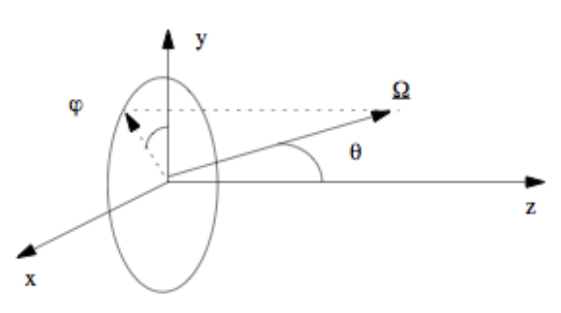
\includegraphics[width=0.4\linewidth]{figures/CartesianOmegaHat.png}
\caption{Definition of \(\theta\) and \(\phi\) in a Cartesian coordinate system. The symbol \(\varphi\) in the figure is used for angular flux in this document, and hence \(\phi\) is used for this angle.}
\label{fig:CartesianOmegaHat}
\end{figure}

Each of these components are often given their own names (caution: the naming convention of \(\xi\) and \(\eta\) differs depending on where you look). 

\begin{equation}
\label{eq:OmegaComponentsCartesian}
\begin{aligned}
 \xi \equiv \textrm{sin}(\theta)\textrm{cos}(\phi)\\
 \eta \equiv \textrm{sin}(\theta)\textrm{sin}(\phi)\\
 \mu \equiv \textrm{cos}(\theta)\\
\end{aligned}
\end{equation}

Using the \(\textrm{sin}^2(\theta) + \textrm{cos}^2(\theta) = 1\) identity, \(\hat{\Omega}\) in Cartesian coordinates can also be written as

\begin{equation}
\label{eq:OmegaCartesianMuOnly}
\hat{\Omega} = \sqrt{1-\mu^2}\textrm{cos}(\phi)\hat{i} + \sqrt{1-\mu^2}\textrm{sin}(\phi)\hat{j} + \mu\hat{k}
\end{equation}

The axes used in 1-D Cartesian problems are often re-oriented such that \(z\) is the independent variable (as opposed to a 1-D problem in \(x\) or a 1-D problem in \(y\)) so that the direction of neutrons is \(\mu\hat{k}\). This convention is the reason why the arguments of the Legendre polynomials in Eq. \ref{eq:LegendrePolynomialDefinitions} are listed as \(\mu\). 

In Cartesian coordinates, a neutron moves along constant \(\hat{\Omega}\) until suffering a collision. This is not the case in curvilinear coordinates. In curvilinear coordinates, which include cylindrical and spherical coordinates, as a neutron streams, the angular coordinates are constantly changing. If this is not intuitive, think of a neutron traveling in a 2-D Cartesian coordinate system along the line \(x = 1\). This neutron moves along constant \(\hat{\Omega}\). However, the same neutron, described in a cylindrical system, is constantly changing its angle relative to the \(x\)-axis. This means that \(\hat{\Omega}\), in the cylindrical coordinate frame, also changes as the neutron moves, even if it hasn't collided with anything!

In a typical Cartesian domain, an incremental volume element is given by \(dV = dxdydz\). Similarly, an incremental solid angle element is given by 

\begin{equation} % why?
\label{eq:DifferentialOmega}
d\hat{\Omega}=\sin{(\theta)}d\theta d\phi=d\mu d\phi
\end{equation}

which represents a dimensionless area on the unit sphere. An integral over \(\hat{\Omega}\) is usually represented shorthand by \(\int_{4\pi}^{ } d\hat{\Omega}\), which represents integration over the entire \(4\pi\) solid angle.

\begin{equation}
\label{eq:4PiOmegaIntegral}
\int_{4\pi}^{ } d\hat{\Omega} = \int_{-1}^{1} d\mu \int_{0}^{2\pi} d\phi = \int_{0}^{\pi} \sin{(\theta)}d\theta \int_{0}^{2\pi} d\phi = 4\pi
\end{equation}

The integral of any two components of the direction vector over \(4\pi\) solid angle gives a condition simliar to an orthogonality statement:

\begin{equation}
\label{eq:4PiOmegaOmega}
\int_{4\pi}^{ } d\hat{\Omega}\Omega_i\Omega_j = \frac{4\pi}{3}\delta_{ij}
\end{equation}

It is frequently assumed that the angular dependence of a collision is rotationally symmetric, which means that scattering cross sections really depend on the \textit{change} in angle between the incident and scattered neutron, rather than the absolute values of each. This assumption is equivalent to assuming that a scattering collision is independent of the angle \(\phi\). In this case, the change in the angle during scattering, where \(\hat{\Omega}\) represents the incident neutron direction and \(\hat{\Omega}'\) represents the scattered neutron direction, can be related to the dot product of the two angles

\begin{equation}
\label{eq:OmegaDotOmega}
\hat{\Omega}\cdot\hat{\Omega}' = |\hat{\Omega}||\hat{\Omega}'| \cos{(\theta)} = \mu
\end{equation} 

where the magnitude of each of the unit direction vectors being 1 has been used. Therefore, the change in angle during scattering is given by \(\mu\) as long as the scattering is rotationally symmetric. This is a second motivation for the use of Legendre polynomials for expansions of the scattering cross section. Expressing cross sections in terms of \(\mu\) implies that we ignore any type of anisotropic grain structure, since on a macroscopic scale, grains are sufficiently randomly oriented. 

\subsubsection{Reaction Rates}

The interaction rate of neutrons is given in terms of an interaction frequency:

\begin{equation}
\label{eq:ReactionFrequency}
\textrm{Reaction Rate Frequency} = v\Sigma
\end{equation}

where \(v\) is the neutron velocity. Intuitively, we see that \(v\) must be included in the interaction frequency; if the velocity were zero, then even if there were many neutrons, none would interact. The reaction rate density is simply

\begin{equation}
\label{eq:ReactionRateDensity}
\textrm{Reaction Rate Density} = v\Sigma N
\end{equation}

where \(N\) is the neutron volumetric density (neutrons/cm\textsuperscript{3}). 

\subsubsection{Flux}

The reaction rate density definition in Eq. \ref{eq:ReactionRateDensity} leads to a convenient \textit{definition} for the angular flux:

\begin{equation}
\label{eq:AngularFlux}
\psi(\vv{r}, E, \hat{\Omega}, t) \equiv v(E)N(\vv{r}, E, \hat{\Omega}, t)
\end{equation}

All angular quantities can be integrated over \(4\pi\) solid angle to give the corresponding ``scalar'' value. The scalar neutron flux is the angular flux with all angular dependence integrated out, also referred to as the zeroth angular moment of the angular flux.

\begin{equation}
\label{eq:ScalarFlux}
\phi(\vv{r}, E, t) = \int_{4\pi}^{} d\hat{\Omega} \psi(\vv{r}, E, \hat{\Omega}, t)
\end{equation}

If the angular flux is isotropic, i.e. independent of angle, then the above integral would simply evaluate to \(\phi(\vv{r}, E, t)=4\pi\psi\). However, the entire crux of neutron transport is that the angular flux usually has strong angular dependence, especially near boundaries or interfaces between regions with very different cross-sections, such as near vacuum boundaries or strong absorbers. 

\subsubsection{Current}

The angular current density has the same magnitude of the angular flux, except that it has direction - it denotes the current of neutrons moving in a certain angular direction:

\begin{equation}
\label{eq:AngularCurrent}
\vv{j}(\vv{r}, E, \hat{\Omega}, t) = \psi(\vv{r}, E, \hat{\Omega}, t)\hat{\Omega}
\end{equation}

The current \(\vv{J}\) is the first angular moment of the angular flux, and is given by:

\begin{equation}
\label{eq:Current}
\vv{J}(\vv{r},E,t)=\int_{4\pi}^{}d\hat{\Omega}\vv{j}=\int_{4\pi}^{}d\hat{\Omega}\psi(\vv{r},E,\hat{\Omega},t)\hat{\Omega}
\end{equation}

To determine how many neutrons cross a unit area, we must integrate the angular current over that area, dotted with the unit normal vector of that surface to indicate that only neutrons moving perpendicular to the surface actually cross it:

\begin{equation}
\label{eq:AngularCurrent}
\textrm{Surface Current} = \int dA \vv{j}(\vv{r}, E, \hat{\Omega}, t)\cdot\hat{n}
\end{equation}

Eq. \ref{eq:AngularCurrent} would then also be integrated over angle and energy to give the total number of neutrons crossing the surface. The fundamental difference between current and flux is that current represents the net rate at which particles stream through a surface (since it is a vector), while flux represents the total rate at which particles stream through a surface, regardless of direction. While Eq. \ref{eq:AngularCurrent} holds for the angular variables, there is no analogous, exact, relationship between \(J\), the scalar current, and \(\phi\). 

Partial currents can be calculated by again dotting the angular current with the surface normal, but this time we can represent outgoing and ingoing current by integration over \(\pm 2\pi\), respectively.

\begin{equation}
\label{eq:PartialCurrent}
J_\pm (\vv{r}, E, t) = \int_{2\pi\pm}^{} d\hat{\Omega} \vv{j}(\vv{r}, E, \hat{\Omega}, t)\cdot\hat{n}
\end{equation}

The net current through a surface is then the sum of the two partial currents (note that \(J_+\) is positive (pointing in the positive direction) while \(J_-\) is negative (pointing in the negative direction), so that we have to actually take the difference between the two to find the net current):

\begin{equation}
\label{eq:TotalCurrent}
J (\vv{r}, E, t) = J_+ - J_-
\end{equation}

\subsection{Pressure Tensor}

While current and scalar flux are the first and zeroth moments of the angular flux, we can also define a second moment of the angular flux as the pressure tensor:

\begin{equation}
\label{eq:PressureTensor}
\bar{\bar{P}}(\vv{r},E,t)=\int_{4\pi}^{}d\hat{\Omega}\hat{\Omega}\hat{\Omega}\psi(\vv{r},\hat{\Omega},E,t)
\end{equation}

\subsection{Legendre Polynomials}

Legendre polynomials \(P_l\) are solutions to:

\begin{equation}
\label{eq:LegendrePolynomialDiffEq}
\frac{d}{d\mu} \left((1-\mu^2) \frac{dP_l}{d\mu}\right) + l(l+1)P_l = 0
\end{equation}

These functions arise from separation of variables of the Laplace equation in spherical coordinates. These functions are commonly used in neutron transport as expansions for the scattering cross section and flux in deterministic methods. These functions are of the form:

\begin{equation}
\label{eq:LegendrePolynomialDefinitions}
P_l (\mu) = \frac{1}{2^l l!} \frac{d^l}{d\mu^l} \left(\mu^2 -1\right)^l
\end{equation}

where \(l\) takes on values of \(0, 1, 2, ..., L\). In neutron transport applications, \(L\) is the order of scattering anisotropy, with \(l=0\) representing isotropic scattering, and \(l = 1\) sometimes being referred to ``linearly anisotropic''. The first several Legendre polynomials are, according to Eq. \ref{eq:LegendrePolynomialDefinitions}

\begin{equation}
\label{eqn:LegendrePolynomials_P0P1P2}
\begin{aligned}
 P_0 (\mu) = 1\\
 P_1 (\mu) = \mu\\
 P_2 (\mu) = \frac{1}{2} (3\mu^2 -1)
\end{aligned}
\end{equation}

An important property of Legendre polynomials is that they are orthogonal on [-1,1], which means that they can be used as a basis over this range. Normally, we would need to do some type of coordinate transformation to ensure that the variable we are expanding in Legendre polynomials only covers the range [-1,1], but fortunately, \(\mu = \cos{(\theta)}\) only covers the range [-1,1]. It is for this reason that we can easily use Legendre polynomials to expand angular-dependent quantities. 

Like other basis functions, Legendre polynomials have an orthogonality property over the range on which they are orthogonal ([-1,1]). This orthogonality property is:

\begin{equation}
\label{eqn:LegendrePolynomialsOrthogonality}
\int_{-1}^{1} d\mu P_l (\mu) P_k (\mu) = \frac{2\delta_{lk}}{2l+1}
\end{equation}

Orthogonality is a very important property, since it allows us to convert infinite sums to single terms due to the Kronecker delta \(\delta_{lk}\) (recall from differential equations classes). Legendre polynomials also satisfy recursion relations that express \(\mu P_l(\mu)\) in terms of only other Legendre polynomials, which is needed in certain derivations in order to then apply orthogonality, which cannot be applied is there is a pesky \(\mu\) remaining in the integral. One of these recursion relations is:

\begin{equation}
\label{eqn:LegendrePolynomialRecursion1}
\mu P_l(\mu) = \frac{1}{2l+1} \left\lbrack(l+1)P_{l+1}(\mu) + l P_{l-1}(\mu)\right\rbrack
\end{equation}

Often in nuclear engineering applications, cross sections and/or neutron flux are ``expanded'' in Legendre polynomials. This means that the angular dependence, previously unknown to us, is now described in terms of Legendre polynomials. This expansion is performed frequently with cross sections so that we do not have to keep cross-section data as a function of angle. Instead, we can store the scattering moments, which are only functions of space and energy, and simply ``look up'' the angle-dependent scattering cross section by evaluating a finite number of Legendre polynomials. To expand a cross section in Legendre polynomials, we write it as an infinite sum of scattering moments \(\Sigma_{s,l}\) with the Legendre polynomials. Because Legendre polynomials are a basis on [-1,1], as long as the series is infinite, no approximation has been made. In practice, however, we would truncate this expression at some finite number of terms. The sum is usually truncated so that its level of approximation matches that being applied to the angular flux. The more anisotropic the scattering cross section, the more incorrect this early truncation becomes. Each extra term that is maintained represents a higher-anisotropy scattering term.

\begin{equation}
\label{eq:ScatteringLegendre}
\Sigma_s(\vv{r}, E'\rightarrow E, \hat{\Omega}'\rightarrow\hat{\Omega}) = \Sigma_s(\vv{r}, E'\rightarrow E, \mu) = \sum_{l=0}^{\infty} \frac{2l+1}{4\pi} \Sigma_{s,l}(\vv{r}, E'\rightarrow E)P_l(\mu)
\end{equation}

% incomplete
Whether or not the \(4\pi\) term always appears in these formulations is not consistent across all texts - its inclusion depends on whether or not (?). Alternatively, Eq. \eqref{eq:ScatteringLegendre} can be phrased as:

\begin{equation}
\label{eq:ScatteringLegendre2}
\Sigma_s(\vv{r}, E'\rightarrow E, \hat{\Omega}'\rightarrow\hat{\Omega}) = \Sigma_s(\vv{r}, E'\rightarrow E, \hat{\Omega}\cdot\hat{\Omega}') = \sum_{l=0}^{\infty} \frac{2l+1}{4\pi} \Sigma_{s,l}(\vv{r}, E'\rightarrow E)P_l(\hat{\Omega}\cdot\hat{\Omega}')
\end{equation}

The scattering moments appearing in Eq. \ref{eq:ScatteringLegendre} can be derived by using the orthogonality condition, Eq. \ref{eqn:LegendrePolynomialsOrthogonality}. Multiplying both sides of Eq. \ref{eq:ScatteringLegendre} by \(P_k(\mu)\) and integrating over \(\mu\), and then applying the results of Eq. \ref{eqn:LegendrePolynomialsOrthogonality} gives

\begin{equation}
\label{eq:ScatteringMomentsLegendre}
\Sigma_{s,l}(\vv{r}, E'\rightarrow E) = 2\pi\int_{-1}^{1} d\mu \Sigma_s(\vv{r}, E'\rightarrow E, \mu) P_l(\mu)
\end{equation}

Again, whether or not the factor of \(2\pi\) appears is dependent on whether or not Eq. \ref{eq:ScatteringLegendre} contains the \(4\pi\) term. Expanding the scattering cross section in Legendre polynomials is known as the \(P_L\) approximation. For neutron and photon transport, we only need the first few terms to obtain sufficient accuracy, though this is not the case for electron scattering, since electrons tend to have much greater anisotropy in scattering than neutrons.

\subsection{Associated Legendre Polynomials}

The Associated Legendre polynomials are more generalized Legendre functions that are the solutions to

\begin{equation}
\label{eq:AssociatedLegendrePolynomialDiffEq}
\frac{d}{d\mu} \left((1-\mu^2) \frac{dP_{lm}}{d\mu}\right) + \left(l(l+1) -\frac{m^2}{1-\mu^2}\right)P_{lm} = 0
\end{equation}

which you will notice is very similar to \ref{eq:LegendrePolynomialDiffEq}, except that now we have an extra parameter, \(0 \leq m \leq l\). Associated Legendre polynomials are central to the definition of the spherical harmonics functions. In general, \(l\) and \(m\) can be real, complex, and non-integer, but the Associated Legendre polynomials reduce to the Legendre polynomials when \(m=0\) and \(l\) is an integer. The Associated Legendre polynomials have the form:

\begin{equation}
\label{eq:AssociatedLegendre}
P_{lm}(\mu)=\frac{(-1)^m}{2^ll!}(1-\mu^2)^{m/2}\frac{d^{l+m}}{d\mu^{l+m}}(\mu^2-1)^l
\end{equation}

The Associated Legendre polynomials are related to each other for \(\pm m\) by:

\begin{equation}
\label{eq:relatingALP}
P_{l,-m}=(-1)^m\frac{(l-m)!}{(l+m)!}P_{lm}
\end{equation}




\subsubsection{Orthogonality}

The Associated Legendre polynomials satisfy the following orthogonality relation:

\begin{equation}
\label{eq:AssociatedLegendreOthogonality}
\int_{-1}^{1}P_{lm}(\mu)P_{l'm'}(\mu)d\mu=\frac{2}{2l+1}\frac{(l+m)!}{(l-m)!}\delta_{ll'}
\end{equation}





\subsection{Spherical Harmonics}

The spherical harmonics functions are eigenfunctions of the monoenergetic Boltzmann scattering operator, and hence serve as a natural basis for expanding the scattering cross section in the transport equation. In order to derive several of the methods used for solving the neutron transport equation, theorems and proofs related to the spherical harmonics are needed. These proofs are collected here to serve as a reference.

The spherical harmonics are defined in terms of the Associated Legendre polynomials given in Eq. \eqref{eq:AssociatedLegendre}. For \(m=0\), or the condition of azimuthal symmetry, the spherical harmonics reduce to the Legendre polynomials. Note that some sources place the \((-1)^m\) factor in the definition of the Associated Legendre polynomials. 

\begin{equation}
\label{eq:SphericaltoAssociated}
Y_{lm}(\theta,\phi)=(-1)^m\sqrt{\frac{(2l+1)}{4\pi}\frac{(l-m)!}{(l+m)!}}P_{lm}(\cos{(\theta)})\exp{(im\phi)}
\end{equation}

Or, in shorthand notation that will be used in later derivations:

\begin{equation}
\label{eq:SphericaltoAssociatedShort}
Y_{lm}(\theta,\phi)=C_{lm}P_{lm}(\cos{(\theta)})\exp{(im\phi)}
\end{equation}

where

\begin{equation}
\label{eq:Clm}
C_{lm}=(-1)^m\sqrt{\frac{(2l+1)}{4\pi}\frac{(l-m)!}{(l+m)!}}
\end{equation}



\subsubsection{Addition Theorem}
The addition theorem of spherical harmonics relates the Legendre polynomials to the spherical harmonic and its complex conjugate. 

\begin{equation}
\label{eq:SHAdditionTheorem}
P_l(\hat{\Omega}'\cdot\hat{\Omega}) = \frac{4\pi}{2l+1} \sum_{m=-l}^{l} Y_{lm}^{*} (\hat{\Omega}') Y_{lm}(\hat{\Omega})
\end{equation}

Eq. \eqref{eq:SHAdditionTheorem} can be split up even further into positive, zero, and negative components of \(m\):

\begin{equation}
\label{eq:SphericalHarmonics2}
P_l(\hat{\Omega}'\cdot\hat{\Omega})=\frac{4\pi}{2l+1}\left\lbrack Y_{l0}(\hat{\Omega})Y_{l0}(\hat{\Omega}')+\sum_{m=1}^{l}\left(Y_{lm}(\hat{\Omega})Y_{lm}^*(\hat{\Omega}')+Y_{l,-m}(\hat{\Omega})Y_{l,-m}^*(\hat{\Omega}')\right)\right\rbrack
\end{equation}

Note that the \(m=0\) term has no complex conjugate symbol on either term because, for \(m=0\), the complex portion of \(Y_{lm}\) is zero based on \(\sin{(0}=0\) in Eq. \eqref{eq:RealImaginary}. 



\begin{tcolorbox}[breakable]
For 1-D geometries, the addition theorem in Eq. \eqref{eq:SphericalHarmonics2} can be simplified, since \(m\neq0\) represents azimuthal dependencies. In 1-D, there are no azimuthal dependencies, which reduces Eq. \eqref{eq:SphericalHarmonics2} to:

\begin{equation}
\label{eq:SphericalHarmonics3}
P_l(\hat{\Omega}'\cdot\hat{\Omega})=\frac{4\pi}{2l+1}\left\lbrack Y_{l0}(\hat{\Omega})Y_{l0}(\hat{\Omega}')+\sum_{m=1}^{l}\left(\cancel{Y_{lm}(\hat{\Omega})Y_{lm}^*(\hat{\Omega})}+\cancel{Y_{l,-m}(\hat{\Omega})Y_{l,-m}^*(\hat{\Omega}')}\right)\right\rbrack
\end{equation}

From Eq. \eqref{eq:SphericaltoAssociated}, \(Y_{l0}\) can be expressed in terms of the Associated Legendre polynomials:

\begin{equation}
\label{eq:SphericalHarmonics4}
P_l(\hat{\Omega}'\cdot\hat{\Omega})=\frac{4\pi}{2l+1}\left\lbrack \sqrt{\frac{2l+1}{4\pi}}P_{l0}(\mu)\sqrt{\frac{2l+1}{4\pi}}P_{l0}(\mu')\right\rbrack\\
\end{equation}

Then, from Eq. \eqref{eq:AssociatedLegendre}, it can be seen that the Associated Legendre polynomials reduce to the Legendre polynomials for \(m=0\). This gives the simplified form of the addition theorem which applies for 1-D geometries:

\begin{equation}
\label{eq:AddSpherical1D}
P_l(\hat{\Omega}'\cdot\hat{\Omega})=P_{l}(\mu)P_{l}(\mu')
\end{equation}

\end{tcolorbox}



Eq. \eqref{eq:SphericaltoAssociated} will let us decompose the \(Y_{l0}\) terms appearing in Eq. \eqref{eq:SphericalHarmonics2}:

\begin{equation}
Y_{l0}=\sqrt{\frac{(2l+1)}{4\pi}}P_{l0}= Y_{l0}^e
\end{equation}

where Eq. \eqref{eq:SphericalHarmonicsEvenOdd} has been used to show that \(Y_{l0}=Y_{l0}^e\).



\subsubsection{Orthogonality}
The spherical harmonics form a basis over \(0\leq\phi\leq2\pi, 0\leq\theta\leq\pi\). Hence, the orthogonality property of spherical harmonics is given as:

\begin{equation}
\label{eq:SHOrthogonality}
\int_{4\pi}^{} d\hat{\Omega} Y_{lm}(\hat{\Omega}) Y_{l'm'}^{*}(\hat{\Omega}) = \delta_{ll'}\delta_{mm'}
\end{equation}



\subsubsection{Expansions of Other Variables}

In general, any arbitrary function \(f\) can be expanded in spherical harmonics:

\begin{equation}
\label{eq:SphericalHarmonicsGeneralExpansion}
f(\hat{\Omega})=\sum_{l=0}^{N}\sum_{m=-l}^{l}Y_{lm}(\hat{\Omega})f_{lm}
\end{equation}

where \(f_{lm}\) are the moments of \(f\). These moments are computed as:

\begin{equation}
\label{eq:SHGeneralMoments}
f_{lm}=\int_{4\pi}^{}f(\hat{\Omega})Y_{lm}^{*}(\hat{\Omega})d\hat{\Omega}
\end{equation}

\begin{tcolorbox}[breakable]
To show Eq. \eqref{eq:SHGeneralMoments}, multiply Eq. \eqref{eq:SphericalHarmonicsGeneralExpansion} by \(Y_{lm}^{*}\) and integrate over \(\hat{\Omega}\):

\begin{equation}
\int_{4\pi}^{}f(\hat{\Omega})Y_{lm}^{*}(\hat{\Omega})d\hat{\Omega}=\int_{4\pi}^{}\sum_{l=0}^{N}\sum_{m=-l}^{l}f_{lm}Y_{lm}(\hat{\Omega})Y_{lm}^{*}(\hat{\Omega})d\hat{\Omega}\rightarrow f_{lm}
\end{equation}

where the orthogonality property from Eq. \eqref{eq:SHOrthogonality} is used to convert the RHS.
\end{tcolorbox}

The expansion in Eq. \eqref{eq:SphericalHarmonicsGeneralExpansion} contains both real and imaginary components, and for real functions such as the scattering source, the imaginary component must be removed. 

\begin{tcolorbox}[breakable]
The moments in Eq. \eqref{eq:SHGeneralMoments}, before removing the imaginary component to the expansion in Eq. \eqref{eq:SphericalHarmonicsGeneralExpansion}, have a real component \(\alpha_{lm}\) and an imaginary component \(\beta_{lm}\) such that:

\begin{equation}
\label{eq:GeneralComplexNumber}
f_{lm}=\alpha_{lm}+i\beta_{lm}
\end{equation}

From the definition in Eq. \eqref{eq:SphericalHarmonicsGeneralExpansion}, the expansion can be broken up into positive and negative components of \(m\), where Eq. \eqref{eq:SphericaltoAssociatedShort} is used for shortening the spherical harmonics:

\begin{equation}
\label{eq:BeginningExpansion1}
f(\hat{\Omega})=\sum_{l=0}^{N}\sum_{m=0}^{l}\left\lbrack C_{lm}P_{lm}(\hat{\Omega})f_{lm}\exp{(im\phi)}+C_{l,-m}P_{l,-m}(\hat{\Omega})f_{l,-m}\exp{(-im\phi)}\right\rbrack
\end{equation}

Because \(\exp{(im\phi)}=\cos{(m\phi)}+i\sin{(m\phi)}\), the above equation can be further expanded by recognizing that \(Y_{lm}\) can be equivalently expressed as:

\begin{equation}
\label{eq:RealImaginary}
\begin{aligned}
Y_{lm}(\hat{\Omega})=C_{lm}P_{lm}(\hat{\Omega})\left(\cos{(m\phi)}+i\sin{(m\phi)}\right)=\hat{Y}_{lm}^e+i\hat{Y}_{lm}^o\\
\hat{Y}_{lm}^e=C_{lm}P_{lm}\cos{(m\phi)}\\
\hat{Y}_{lm}^o=C_{lm}P_{lm}\sin{(m\phi)}\\
\end{aligned}
\end{equation}

Inserting Eq. \eqref{eq:RealImaginary} into Eq. \eqref{eq:BeginningExpansion1}:

\begin{equation}
f(\hat{\Omega})=\sum_{l=0}^{N}\sum_{m=0}^{l}\left\lbrack C_{lm}P_{lm}(\hat{\Omega})f_{lm}\left(\cos{(m\phi)}+i\sin{(m\phi)}\right)+C_{l,-m}P_{l,-m}(\hat{\Omega})f_{l,-m}\left(\cos{(m\phi)}-i\sin{(m\phi)}\right)\right\rbrack
\end{equation}

where the fact that cosine is an even function and sine an odd function has been used in the second term. Then, inserting Eq. \eqref{eq:GeneralComplexNumber} and grouping the terms by real and imaginary components:

\begin{equation}
\label{eq:FullExpansionSH}
\begin{aligned}
f(\hat{\Omega})=\sum_{l=0}^{N}\sum_{m=0}^{l}\left[ \text{Real}+i\left(\text{Imag}\right)\right]\\
\text{Real} = C_{lm}P_{lm}(\hat{\Omega})\left(\alpha_{lm}\cos{(m\phi)}-\beta_{lm}\sin{(m\phi)}\right)+C_{l,-m}P_{l,-m}(\hat{\Omega})\left(\alpha_{l,-m}\cos{(m\phi)}+\beta_{l,-m}\sin{(m\phi)}\right)\\
\text{Imag} = C_{lm}P_{lm}(\hat{\Omega})\left(\alpha_{lm}\sin{(m\phi)}+\beta_{lm}\cos{(m\phi)}\right)+C_{l,-m}P_{l,-m}(\hat{\Omega})\left(\beta_{l,-m}\cos{(m\phi)}-\alpha_{l,-m}\sin{(m\phi)}\right)\\\
\end{aligned}
\end{equation}

For physically-meaningful quantities such as the scattering source, the expansion must contain only real terms. Hence, all imaginary terms go to zero. For the imaginary term above to be zero for all \(\phi\), the coefficients on the two linearly independent functions \(\sin{(m\phi)}\) and \(\cos{(m\phi)}\) must be zero. This leads to the following two conditions:

\begin{equation}
\begin{aligned}
C_{lm}P_{lm}(\hat{\Omega})\alpha_{lm}-C_{l,-m}P_{l,-m}(\hat{\Omega})\alpha_{l,-m}=0\\
C_{lm}P_{lm}(\hat{\Omega})\beta_{lm}+C_{l,-m}P_{l,-m}(\hat{\Omega})\beta_{l,-m}=0\\
\end{aligned}
\end{equation}

Using these conditions to eliminate terms with \(-m\) in Eq. \eqref{eq:FullExpansionSH} (with the imaginary component removed), the real expansion of \(f\) becomes:

\begin{equation}
\label{eq:FullExpansionSH2}
f(\hat{\Omega})=\sum_{l=0}^{N}\sum_{m=0}^{l}C_{lm}P_{lm}(\hat{\Omega})\left(2\alpha_{lm}\cos{(m\phi)}-2\beta_{lm}\sin{(m\phi)}\right)
\end{equation}

The new basis for the real expansion of \(f\) consists of the two ``hatted'' functions in Eq. \eqref{eq:RealImaginary}. These hatted functions represent a basis, and hence must be orthogonal over the unit sphere. This requirement holds for both the even and odd functions separately. Multiplying \(\hat{Y}_{lm}^e\) by itself and integrating over the unit sphere, and then applying the orthogonality condition in Eq. \eqref{eq:SHOrthogonality}:

\begin{equation}
\label{eq:EvenRequriedOrthogonality}
\int_{4\pi}^{}\hat{Y}_{lm}^e\hat{Y}_{l'm'}^ed\hat{\Omega}=C_{lm}^2\int_{0}^{2\pi}\cos{(m\phi)}\cos{(m'\phi)}d\phi\int_{-1}^{1}P_{lm}P_{lm'}d\mu
\end{equation}

The orthogonality property of cosines functions is:

\begin{equation}
\int_{0}^{2\pi}\cos{(m\phi)}\cos{(m'\phi)}d\phi=\pi(1+\delta_{m0})\delta_{mm'}
\end{equation}

Using this cosine orthogonality property and the Legendre polynomial orthogonality from Eq. \eqref{eq:AssociatedLegendreOrthogonality} in Eq. \eqref{eq:EvenRequriedOrthogonality} gives:

\begin{equation}
\label{eq:EvenRequriedOrthogonality2}
\int_{4\pi}^{}\hat{Y}_{lm}^e\hat{Y}_{l'm'}^ed\hat{\Omega}=\frac{1}{2}(1+\delta_{m0})\delta_{mm'}\delta_{ll'}
\end{equation}

where the definition for \(C_{lm}\) from Eq. \eqref{eq:Clm} has been inserted. In order for the \(\hat{Y}_{lm}^e\) to be orthogonal, the above resulting constant, multiplied by some unknown constant \(\mathscr{C}^2\), must give 1. 

\begin{equation}
\mathscr{C}^2\frac{1}{2}(1+\delta_{m0})\delta_{mm'}\delta_{ll'}=1
\end{equation}

This gives two possible solutions, one for \(m=0\) and one for \(m\neq 0\). For \(m=0\), \(\mathscr{C}=1\), and for \(m\neq0\), \(\mathscr{C}=\sqrt{2}\). The only way both of these can be satisfied is if:

\begin{equation}
\mathscr{C}=\sqrt{2-\delta_{m0}}
\end{equation}

Similarly, the odd \(\hat{Y}_{lm}\) have to be orthogonal over the unit sphere. The orthogonality property of sine functions is stated as:

\begin{equation}
\label{eq:SineOrthogonality}
\int_{0}^{2\pi}\sin{(m\phi)}\sin{(m'\phi)}d\phi=\pi(1-\delta_{m0})\delta_{mm'}
\end{equation}

Multiplying \(\hat{Y}_{lm}^o\) by itself and then integrating over \(4\pi\) gives:

\begin{equation}
\label{eq:OddRequriedOrthogonality2}
\int_{4\pi}^{}\hat{Y}_{lm}^o\hat{Y}_{l'm'}^od\hat{\Omega}=\frac{1}{2}\delta_{ll'}(1-\delta_{m0})\delta_{mm'}
\end{equation}

where the definition for \(C_{lm}\) from Eq. \eqref{eq:Clm}, the Associated Legendre polynomial orthogonality property from Eq. \eqref{eqn:AssociatedLegendreOrthogonality}, and the sine orthogonality property from Eq. \eqref{eq:SineOrthogonality} have been used. In order for the odd basis functions to be orthogonal, the resulting above constant, multiplied by some constant \(\mathscr{C}\), must equal 1. Hence, a second condition similar to that obtained for the even functions is obtained:

\begin{equation}
\mathscr{C}^2\frac{1}{2}\delta_{ll'}(1-\delta_{m0})\delta_{mm'}=1
\end{equation} 

This gives two solutions - for \(m=0\), the odd functions are identically zero. For \(m\neq0\), \(\mathscr{C}=1/\sqrt{2}\), the same result obtained for the even functions. Hence, while the imaginary and complex expansion is defined in Eq. \eqref{eq:RealImaginary}, the real basis for \(f\) is determined by multiplying \(\hat{Y}_{lm}^e\) and \(\hat{Y}_{lm}^o\) by \(\mathscr{C}\) to give:

\begin{equation}
\label{eq:RealExpansionSH}
\begin{aligned}
Y_{lm}^e=\sqrt{2-\delta_{m0}}C_{lm}P_{lm}\cos{(m\phi)}\\
Y_{lm}^o=\sqrt{2-\delta_{m0}}C_{lm}P_{lm}\sin{(m\phi)}\\
\end{aligned}
\end{equation}

where the real expansion functions is distinguished from the complex expansion by not including ``hats.'' By comparing Eq. \eqref{eq:RealExpansionSH} with Eq. \eqref{eq:RealImaginary}, it is clear that:

\begin{equation}
\label{eq:HattoNoHat}
\begin{aligned}
Y_{lm}^e=\sqrt{2-\delta_{m0}}\hat{Y}_{lm}^e\\
Y_{lm}^o=\sqrt{2-\delta_{m0}}\hat{Y}_{lm}^o\\
\end{aligned}
\end{equation}

And because the odd functions are zero for \(m=0\), the second line above could equivalently be stated as \(Y_{lm}^o=\sqrt{2}\hat{Y}_{lm}^o\) with the understanding that \(Y_{lm}\) is zero for \(m=0\). 

\end{tcolorbox}



\begin{tcolorbox}[breakable]
We can also express \(\hat{Y}_{lm}^e\) in terms of \(\hat{Y}_{l,-m}^e\) using the definition in Eq. \eqref{eq:RealImaginary}. 

\begin{equation}
\begin{aligned}
\hat{Y}_{lm}^e=(-1)^m\sqrt{\frac{2l+1}{4\pi}\frac{(l-m)!}{(l+m)!}}P_{lm}\cos{(m\phi)}\\
\hat{Y}_{l,-m}^e=(-1)^{-m}\sqrt{\frac{2l+1}{4\pi}\frac{(l-(-m))!}{(l+(-m))!}}P_{l,-m}\cos{(-m\phi)}\\
\end{aligned}
\end{equation}

The \(\hat{Y}_{l,-m}^e\) term can be further simplified to the following, 

\begin{equation}
\begin{aligned}
\hat{Y}_{l,-m}^e=(-1)^{2m}\sqrt{\frac{2l+1}{4\pi}\frac{(l-m))!}{(l+m)!}}P_{lm}\cos{(m\phi)}\\
\end{aligned}
\end{equation}

where \(P_{l,-m}\) is related to \(P_{lm}\) by Eq. \eqref{eq:relatingALP} and the fact that cosine is an even function has been used. Hence, it can be seen that:

\begin{equation}
\label{eq:MinusMtoM}
\hat{Y}_{l,-m}^e=(-1)^m\hat{Y}_{lm}^e
\end{equation}

Likewise, 

\begin{equation}
\label{eq:MinusMtoMOdd}
\hat{Y}_{l,-m}^o=-(-1)^m\hat{Y}_{lm}^o
\end{equation}

\end{tcolorbox}



In order to remove the imaginary components in Eq. \eqref{eq:SphericalHarmonics2}, express the summation in terms of ``hatted'' spherical harmonics as shown in Eq. \eqref{eq:RealImaginary}:

\begin{equation}
\begin{aligned}
\label{eq:FullExpansion}
P_l(\hat{\Omega}'\cdot\hat{\Omega})=\frac{4\pi}{2l+1}\left\lbrack \left(\hat{Y}_{l0}^e(\hat{\Omega})+i\cancel{\hat{Y}_{l0}^o(\hat{\Omega})}\right)\left(\hat{Y}_{l0}^e(\hat{\Omega}')+i\cancel{\hat{Y}_{l0}^o(\hat{\Omega}')}\right)\right\rbrack+\\
\frac{4\pi}{2l+1}\left\lbrack\sum_{m=1}^{l}\left(\left(\hat{Y}_{lm}^e(\hat{\Omega})+i\hat{Y}_{lm}^o(\hat{\Omega})\right)\left(\hat{Y}_{lm}^{e*}(\hat{\Omega}')+i\hat{Y}_{lm}^{o*}(\hat{\Omega}')\right)+\left(\hat{Y}_{l,-m}^e(\hat{\Omega})+i\hat{Y}_{l,-m}^o(\hat{\Omega})\right)\left(\hat{Y}_{l,-m}^{e*}(\hat{\Omega}')+i\hat{Y}_{l,-m}^{o*}(\hat{\Omega}')\right)\right)\right\rbrack\\
\end{aligned}
\end{equation}

where from the definition in Eq. \eqref{eq:RealImaginary}, we know that the \(Y_{l0}^o=0\). Because we want the expansion to be real for certain quantities such as the scattering source, all imaginary terms from Eq. \eqref{eq:FullExpansion} are removed to give:

\begin{equation}
\begin{aligned}
\label{eq:FullExpansion2}
P_l(\hat{\Omega}'\cdot\hat{\Omega})=\frac{4\pi}{2l+1}\left\lbrack \hat{Y}_{l0}^e(\hat{\Omega})\hat{Y}_{l0}^e(\hat{\Omega}')+\sum_{m=1}^{l}\left(\hat{Y}_{lm}^e(\hat{\Omega})\hat{Y}_{lm}^{e*}(\hat{\Omega}')-\hat{Y}_{lm}^o(\hat{\Omega})\hat{Y}_{lm}^{o*}(\hat{\Omega}')+\hat{Y}_{l,-m}^e(\hat{\Omega})\hat{Y}_{l,-m}^{e*}(\hat{\Omega}')-\hat{Y}_{l,-m}^o(\hat{\Omega})\hat{Y}_{l,-m}^{o*}(\hat{\Omega}')\right)\right\rbrack\\
\end{aligned}
\end{equation}

Because the odd component is defined as in Eq. \eqref{eq:RealImaginary}, the complex conjugate of \(\hat{Y}_{lm}^o\) simply is equal to the negative of \(\hat{Y}_{lm}^o\) (since the factor of \(i\) in front becomes negative for complex conjugates). Likewise, the complex conjugate of \(\hat{Y}_{lm}^e\) is simply equal to \(\hat{Y}_{lm}^e\) because the even component has no complex terms. In addition, the \(-m\) terms can be related to the \(+m\) terms using Eq. \eqref{eq:MinusMtoM} and \eqref{eq:MinusMtoMOdd}. Hence, the above becomes:

\begin{equation}
\begin{aligned}
\label{eq:FullExpansion3}
P_l(\hat{\Omega}'\cdot\hat{\Omega})=\frac{4\pi}{2l+1}\left\lbrack \hat{Y}_{l0}^e(\hat{\Omega})\hat{Y}_{l0}^e(\hat{\Omega}')+\sum_{m=1}^{l}\left(2\hat{Y}_{lm}^e(\hat{\Omega})\hat{Y}_{lm}^{e}(\hat{\Omega}')+2\hat{Y}_{lm}^o(\hat{\Omega})\hat{Y}_{lm}^{o}(\hat{\Omega}')\right)\right\rbrack\\
\end{aligned}
\end{equation}

From the definitions in Eq. \eqref{eq:HattoNoHat} and Eq. \eqref{eq:HattoNoHat}, the above becomes:

\begin{equation}
\begin{aligned}
\label{eq:FullExpansion4}
P_l(\hat{\Omega}'\cdot\hat{\Omega})=\frac{4\pi}{2l+1}\left\lbrack \hat{Y}_{l0}^e(\hat{\Omega})\hat{Y}_{l0}^e(\hat{\Omega}')+\sum_{m=1}^{l}\left(Y_{lm}^e(\hat{\Omega})Y_{lm}^{e}(\hat{\Omega}')+Y_{lm}^o(\hat{\Omega})Y_{lm}^{o}(\hat{\Omega}')\right)\right\rbrack\\
\end{aligned}
\end{equation}

Finally, using Eq. \eqref{eq:HattoNoHat} and Eq. \eqref{eq:RealExpansionSH}, \(\hat{Y}_{l0}^e=Y_{l0}^e\). This then leads to the final form of the expansion that now contains only real components:

\begin{equation}
\begin{aligned}
\label{eq:FullExpansion5}
P_l(\hat{\Omega}'\cdot\hat{\Omega})=\frac{4\pi}{2l+1}\left\lbrack Y_{l0}^e(\hat{\Omega})Y_{l0}^e(\hat{\Omega}')+\sum_{m=1}^{l}\left(Y_{lm}^e(\hat{\Omega})Y_{lm}^{e}(\hat{\Omega}')+Y_{lm}^o(\hat{\Omega})Y_{lm}^{o}(\hat{\Omega}')\right)\right\rbrack\\
\end{aligned}
\end{equation}





The scattering cross section is often expanded in Legendre polynomials as in Eq. \ref{eq:ScatteringLegendre}, and then the Legendre polynomials in that expansion are themselves expanded in the spherical harmonics using the identity in Eq. \ref{eq:SHAdditionTheorem}. This double expansion takes the form:

\begin{equation}
\label{eq:ScatteringLegendreandSH}
\Sigma_s(\vv{r}, E'\rightarrow E, \hat{\Omega}'\rightarrow\hat{\Omega}) = \Sigma_s(\vv{r}, E'\rightarrow E, \mu) = \sum_{l=0}^{\infty} \Sigma_{s,l}(\vv{r}, E'\rightarrow E) \sum_{m=-l}^{l} Y_{lm}^{*} (\hat{\Omega}') Y_{lm}(\hat{\Omega})
\end{equation}

Further, because the scattering cross section usually appears within an integral with the angular flux, such as in Eq. \ref{eq:ConservationInscatteringSource}, after we perform the spherical harmonics expansion, we can define another quantity, the flux moments:

\begin{equation}
\label{eq:FluxMomentSH}
\phi_l^m(\vv{r}, E, t) = \int_{4\pi}^{} d\hat{\Omega}'\psi(\vv{r}, E', \hat{\Omega}', t)Y_l^{m*}(\hat{\Omega}')
\end{equation}

\section{Derivation of the Transport Equation in Various Geometries}

The transport equation can be derived from conservation principles in an arbitrary control volume \(V\). We will derive the equation in terms of neutron density \(N\) since we are really conserving the number of neutrons, and not the flux itself. The neutron density is in general a function of \(\vv{r}, E, \hat{\Omega}, \) and \(t\), and hence the neutron transport equation is, in general, a 7-dimensional equation (3 spatial variables, 2 angular variables, 1 energy variable, and 1 time variable). It is this rich phase space that makes solving the neutron transport equation so difficult. 

Assuming neutrons are conserved, the time rate of change of neutrons in the control volume equals the net change of neutrons in the control volume. 

\begin{equation}
\label{eq:Conservation1}
\frac{\partial}{\partial t} \left\lbrack\int dV N(\vv{r}, E, \hat{\Omega},t)\right\rbrack dEd\hat{\Omega} = \textrm{gain} - \textrm{loss}
\end{equation}

Because \(N\) is a density per cm\textsuperscript{3}, the amount of neutrons in the \textit{space} of the control volume is only dictated by an integral over \(dV\), which is why we can simply multiply the entire expression by \(dEd\hat{\Omega}\). This is performed similarly for the other terms in the transport equation that are derived below. Assuming the shape of the control volume does not change in time, then the time derivative can be brought inside the integral.

\begin{equation}
\label{eq:Conservation2}
\left\lbrack\int dV \frac{\partial N(\vv{r}, E, \hat{\Omega},t) }{\partial t}\right\rbrack dEd\hat{\Omega} = \textrm{gain} - \textrm{loss}
\end{equation}

The sources of neutrons in the control volume can come from external sources whose magnitude are independent of the neutron density itself, inscattering from other energy groups, prompt fission neutrons, and delayed neutrons. The external source gain is

\begin{equation}
\label{eq:ConservationExternalSource}
\textrm{external source} = \left\lbrack\int dV S(\vv{r}, E, \hat{\Omega},t)\right\rbrack dEd\hat{\Omega}
\end{equation}

The inscattering source gain is an integral over all possible neutron energies \(E'\) and angles \(\hat{\Omega}'\), since theoretically any other neutron could scatter into another neutron energy group. A reaction frequency is given, in units of time, as in Eq. \ref{eq:ReactionFrequency}. The rate at which interactions, such as inscattering, occur is directly controlled by this frequency, and hence the reaction frequency will appear in all terms related to reactions in the transport equation.

\begin{equation}
\label{eq:ConservationInscatteringSource}
\textrm{inscattering source} = \left\lbrack\int_{0}^{\infty} dE'\int_{4\pi}^{} d\hat{\Omega}'\int dV v(E')\Sigma_s(\vv{r},E'\rightarrow E, \hat{\Omega}'\rightarrow\hat{\Omega}) N(\vv{r}, E', \hat{\Omega}',t)\right\rbrack dEd\hat{\Omega}
\end{equation}

The fission source is also an integral over all possible neutron energies and angles, since fission can theoretically be caused by a neutron of any energy. Because neutrons from fission are born (very nearly) isotropically, we can avoid writing another integral over angle and simply divide the prompt fission yield spectrum \(\chi_p(E)\) by \(4\pi\). The fraction of neutrons born delayed is given as \(\beta\), which we must be accounted for separately because we are using the prompt fission neutron spectrum.

\begin{equation}
\label{eq:ConservationFissionPrompt}
\textrm{(prompt) fission source} = \left\lbrack\frac{\chi_p(E)}{4\pi} \int_{0}^{\infty} dE'\int_{4\pi}^{} d\hat{\Omega}'\int dV (1-\beta(E'))\nu(E')v(E')\Sigma_f(\vv{r},E')N(\vv{r}, E, \hat{\Omega},t)\right\rbrack dEd\hat{\Omega}
\end{equation}

The delayed neutron source is the sum of the delayed neutrons from \(J\) delayed neutron precursor groups, where each group has a decay constant \(\lambda\) from a precursor with concentration \(C\) with a neutron energy spectrum \(\chi_d\). \(J\) is customarily taken to be 6.

\begin{equation}
\label{eq:ConservationFissionDelayed}
\textrm{(delayed) fission source} = \left\lbrack\int dV \sum_{j=1}^{J} \frac{\chi_{d,j}(E)}{4\pi} \lambda_j C_j(\vv{r}, t)\right\rbrack dEd\hat{\Omega}
\end{equation}

The losses from the control volume include absorption and streaming (leakage). Instead of including simply an absorption term as a loss, however, we need to balance the inscattering term in Eq. \ref{eq:ConservationInscatteringSource}. This equation has no indication of whether or not the neutron scattering caused it to leave an energy group - in fact, it still contains within-group scattering, which should not be counted as a gain. For this reason, we will subtract as a loss the sum of absorption and outscattering from the present energy group to all other energy groups, \textit{including inscattering}, as this will balance the double counting of within-group scatterings. 

\begin{equation}
\label{eq:ConservationTotal}
\textrm{absorption and outscattering loss}=\left\lbrack\int dV v(E)\Sigma_t(\vv{r}, E) N(\vv{r}, E, \hat{\Omega},t)\right\rbrack dEd\hat{\Omega}
\end{equation}

where \(\Sigma_t=\Sigma_a+\Sigma_s\) is the total cross section, and \(\Sigma_s\) indicates the total scattering probability from an energy group \(E\) to any other energy group, including its own group. 

Finally, neutron streaming from the control volume is only a function of the neutrons that move perpendicularly to the bounding surface, since neutrons moving parallel to the surface are not actually leaving the control volume. Because the direction of the neutrons is what is important in this case, we should integrate the product of the angular current, defined in Eq. \eqref{eq:AngularCurrent}, over the surface area, dotted with the unit normal vector of the surface. 

\begin{equation}
\label{eq:ConservationStreaming1}
\textrm{streaming loss} = \left\lbrack\int dA \vv{j}(\vv{r}, E, \hat{\Omega},t)\cdot \hat{n}\right\rbrack dEd\hat{\Omega}=\left\lbrack\int dA v(E)N(\vv{r}, E, \hat{\Omega},t)\hat{\Omega}\cdot \hat{n}\right\rbrack dEd\hat{\Omega}
\end{equation}

where the angular flux definition in Eq. \eqref{eq:AngularFlux} has been used. Apply the divergence theorem so that this integral becomes a volume integral instead of an area integral:

\begin{equation}
\label{eq:ConservationStreaming2}
\textrm{streaming loss} =\left\lbrack\int dV \hat{\Omega}\cdot\nabla\left(v(E)N(\vv{r}, E, \hat{\Omega},t)\right)\right\rbrack dEd\hat{\Omega}
\end{equation}

Combining all of these terms together yields the transport equation. \(dEd\hat{\Omega}\) cancels in every term. Because all the integrals are over \(dV\), the only way for the entire expression to always be true is if the integrand of the term to go to zero, since the selection of the specific control volume was arbitrary. This leads to the integro-differential transport equation, which is named as such because it contains both integrals and derivatives. Note also that neutron density \(N\) has been replaced with angular flux according to the definition in Eq. \eqref{eq:AngularFlux}. This is also known as the linear Boltzmann transport equation, because we have neglected any nonlinearities due to neutron-neutron interactions. 

\begin{equation}
\label{eq:TE}
\begin{aligned}
\frac{1}{v(E)} \frac{\partial\psi(\vv{r}, E, \hat{\Omega},t)}{\partial t} +
 \hat{\Omega}\cdot\nabla\psi(\vv{r}, E, \hat{\Omega},t) + 
 \Sigma_t(\vv{r},E)\psi(\vv{r}, E, \hat{\Omega},t) = \\
S(\vv{r}, E, \hat{\Omega},t) + \int_{0}^{\infty}dE' \int_{4\pi}^{ } d\hat{\Omega}' \Sigma_s(\vv{r}, E'\rightarrow E, \hat{\Omega}'\rightarrow\hat{\Omega})\psi(\vv{r}, E', \hat{\Omega}',t) + \\
 \frac{\chi_p(E)}{4\pi} \int_{0}^{\infty} dE'\int_{4\pi}^{} d\hat{\Omega}'(1-\beta(E'))\nu(E')\Sigma_f(\vv{r}, E')\psi(\vv{r}, E', \hat{\Omega}',t) + 
 \sum_{j = 1}^{J} \frac{\chi_{d,j}(E)}{4\pi} \lambda_j C_j(\vv{r}, t))
\end{aligned}
\end{equation}

From here moving forward, the distinction between prompt and delayed source will be neglected, and the fission source will be lumped together as a single term with a single spectrum \(\chi_p\). Most codes do not separately treat the prompt and delayed sources, but rather use great simplifications such as point kinetics to avoid working with the very complicated transport equation in kinetics problems. 

Eq. \eqref{eq:TE} is commonly written in one of two forms, since the form in Eq. \eqref{eq:TE} is extremely difficult to solve as-is. The fixed-source form removes all time dependence and the fission source to create a form that is used to solve shielding problems for which a known source drives the results:

\begin{equation}
\label{eq:TE_fixedsource}
\begin{aligned}
 \hat{\Omega}\cdot\nabla\psi(\vv{r}, E, \hat{\Omega},t) + 
 \Sigma_t(\vv{r},E)\psi(\vv{r}, E, \hat{\Omega},t) = \\
S(\vv{r}, E, \hat{\Omega},t) + \int_{0}^{\infty}dE' \int_{4\pi}^{ } d\hat{\Omega}' \Sigma_s(\vv{r}, E'\rightarrow E, \hat{\Omega}'\rightarrow\hat{\Omega})\psi(\vv{r}, E', \hat{\Omega}',t)\\
\end{aligned}
\end{equation}

Alternatively, Eq. \eqref{eq:TE} is frequently expressed in eigenvalue form, where \(k\) is the eigenvalue. Time dependence is also removed as in the fixed source problem, but now the external source, rather than the fission source, is removed, since eigenvalue problems represent situations for which there is no external source.

\begin{equation}
\label{eq:TE_eigenvalue}
\begin{aligned}
 \hat{\Omega}\cdot\nabla\psi(\vv{r}, E, \hat{\Omega},t) + 
 \Sigma_t(\vv{r},E)\psi(\vv{r}, E, \hat{\Omega},t) = \\
\int_{0}^{\infty}dE' \int_{4\pi}^{ } d\hat{\Omega}' \Sigma_s(\vv{r}, E'\rightarrow E, \hat{\Omega}'\rightarrow\hat{\Omega})\psi(\vv{r}, E', \hat{\Omega}',t) + \\
 \frac{1}{k}\left\lbrack\frac{\chi_p(E)}{4\pi} \int_{0}^{\infty} dE'\int_{4\pi}^{} d\hat{\Omega}'(1-\beta(E'))\nu(E')\Sigma_f(\vv{r}, E')\psi(\vv{r}, E', \hat{\Omega}',t) + 
 \sum_{j = 1}^{J} \frac{\chi_{d,j}(E)}{4\pi} \lambda_j C_j(\vv{r}, t))\right\rbrack
\end{aligned}
\end{equation}

And, although the form in Eq. \eqref{eq:TE} appears very daunting, it is a simple expression of conservation of neutrons. By removing the time-dependent term and combining the fission and external sources together into \(q\), integrating over space, angle, and energy reduces Eq. \eqref{eq:TE} to:

\begin{equation}
\nabla\cdot\vv{J}(\vv{r})+(\Sigma_t(\vv{r})-\Sigma_s(\vv{r}))\phi(\vv{r})=q(\vv{r})
\end{equation}

\subsubsection{Boundary Conditions}

This section discusses the boundary conditions used in Eq. \eqref{eq:TE}. The incoming flux \(\psi_{inc}\) can be specified for incoming directions:

\begin{equation}
\psi(\vv{r},\hat{\Omega},E,t)=\psi_{inc}\quad\vv{r}\in \partial V\quad\hat{\Omega}\cdot\hat{n}<0
\end{equation}

where \(\partial V\) is a common way of denoting one lower dimension than the problem domain \(V\). Hence, if the problem is 2-D, \(V\) represents the two-dimensional domain, while \(\partial V\) represents the one-dimensional boundaries. For eigenvalue problems, \(\psi_{inc}=0\) on all boundaries because an eigenvalue problem is defined such that there are no external sources present. 

All problems can also specify reflecting conditions:

\begin{equation}
\psi(\vv{r},\hat{\Omega},E,t)=\psi(\vv{r},-\hat{\Omega},E,t)\quad\vv{r}\in\partial V
\end{equation}

\subsection{Legendre Polynomial and Spherical Harmonics Expansions}
This section will show how to reduce Eq. \eqref{eq:TE} to simpler forms by expanding cross sections and flux in Legendre polynomials or spherical harmonics.

\subsubsection{Legendre Polynomials}

By expanding the scattering cross section in Legendre polynomials as in Eq. \ref{eq:ScatteringLegendre}, we obtain:

\begin{equation}
\label{eq:TEPLnoSHwithPL}
\begin{aligned}
\frac{1}{v(E)} \frac{\partial\psi(\vv{r}, E, \hat{\Omega},t)}{\partial t} +
 \hat{\Omega}\cdot\nabla\psi(\vv{r}, E, \hat{\Omega},t) + 
 \Sigma_t(\vv{r},E)\psi(\vv{r}, E, \hat{\Omega},t) = \\
 \int_{0}^{\infty}dE' \sum_{l=0}^{\infty} \frac{2l+1}{4\pi}\Sigma_{s,l}(\vv{r}, E'\rightarrow E) \int_{4\pi}^{} d\hat{\Omega}'P_l(\hat{\Omega}'\cdot\hat{\Omega})\psi(\vv{r}, E', \hat{\Omega}', t) + S(\vv{r}, E, \hat{\Omega},t)+\\
  \frac{\chi_p(E)}{4\pi} \int_{0}^{\infty} dE'\int_{4\pi}^{} d\hat{\Omega}'\nu(E')\Sigma_f(\vv{r}, E')\psi(\vv{r}, E', \hat{\Omega}',t)\\
\end{aligned}
\end{equation}

\subsubsection{Spherical Harmonics}

Expanding the Legendre polynomials in Eq. \eqref{eq:TEPLnoSHwithPL} in the spherical harmonics, as in Eq. \ref{eq:ScatteringLegendreandSH}, we obtain an equivalent form of the transport equation:

\begin{equation}
\label{eq:TEPLnomoments}
\begin{aligned}
\frac{1}{v(E)} \frac{\partial\psi(\vv{r}, E, \hat{\Omega},t)}{\partial t} +
 \hat{\Omega}\cdot\nabla\psi(\vv{r}, E, \hat{\Omega},t) + 
 \Sigma_t(\vv{r},E)\psi(\vv{r}, E, \hat{\Omega},t) = \\
 \int_{0}^{\infty}dE' \sum_{l=0}^{\infty} \Sigma_{s,l}(\vv{r}, E'\rightarrow E) \sum_{m=-l}^{l} Y_{lm}(\hat{\Omega})\int_{4\pi}^{} d\hat{\Omega}'\psi(\vv{r}, E', \hat{\Omega}', t)Y_l^{m*}(\hat{\Omega}') + S(\vv{r}, E, \hat{\Omega},t)+\\
 \frac{\chi_p(E)}{4\pi} \int_{0}^{\infty} dE'\int_{4\pi}^{} d\hat{\Omega}'\nu(E')\Sigma_f(\vv{r}, E')\psi(\vv{r}, E', \hat{\Omega}',t)\\
\end{aligned}
\end{equation}

The scattering must be real, and hence we can expand the spherical harmonics into positive and negative components of \(m\) to see how we can expand a real-valued term (the scattering integral) in complex functions. 

From Eq. \eqref{eq:TEPLnomoments}, we can further substitute in the definition for the flux moments as in Eq. \ref{eq:FluxMomentSH},  to obtain another equivalent form of the transport equation:

\begin{equation}
\label{eq:TEPL}
\begin{aligned}
\frac{1}{v(E)} \frac{\partial\psi(\vv{r}, E, \hat{\Omega},t)}{\partial t} +
 \hat{\Omega}\cdot\nabla\psi(\vv{r}, E, \hat{\Omega},t) + 
 \Sigma_t(\vv{r},E)\psi(\vv{r}, E, \hat{\Omega},t) = \\
 \int_{0}^{\infty}dE' \sum_{l=0}^{\infty} \Sigma_{s,l}(\vv{r}, E'\rightarrow E) \sum_{m=-l}^{l} Y_{lm}(\hat{\Omega})\phi_l^m(\vv{r}, E, t) + S(\vv{r}, E, \hat{\Omega},t)+\\
\frac{\chi_p(E)}{4\pi} \int_{0}^{\infty} dE'\int_{4\pi}^{} d\hat{\Omega}'\nu(E')\Sigma_f(\vv{r}, E')\psi(\vv{r}, E', \hat{\Omega}',t)\\
\end{aligned}
\end{equation}

\subsection{Integrating Over Angle}

 If we integrate Eq. \ref{eq:TE} over angle, we obtain what is known as the neutron continuity equation:

\begin{equation}
\label{eq:NeutronContinuityEquation}
\begin{aligned}
\frac{1}{v(E)} \frac{\partial\phi(\vv{r}, E, t)}{\partial t} +
 \nabla\cdot J(\vv{r}, E, t) + 
 \Sigma_t(\vv{r},E)\phi(\vv{r}, E, t) = \\
 \int_{0}^{\infty}dE' \Sigma_s(\vv{r}, E'\rightarrow E)\phi(\vv{r}, E', t) + S(\vv{r}, E, t)+\\
 \frac{\chi_p(E)}{4\pi} \int_{0}^{\infty} dE'\nu(E')\Sigma_f(\vv{r}, E')\phi(\vv{r}, E',t)
\end{aligned}
\end{equation}

By integrating over angle, we introduced a new variable - \(J\). Unfortunately, \(J\) cannot be expressed in terms of \(\phi\) in an exact manner, but Eq. \ref{eq:NeutronContinuityEquation} does reduced to the diffusion equation if we make the approximation of Fick's law. If instead we multiplied Eq. \ref{eq:TE} by \(\hat{\Omega}\) and then integrated over angle, we can obtain another equivalent form of the transport equation that will primarily be in terms of current, rather than flux. All source terms (fission, delayed neutrons, and external source) are bundled into \(S\) for simplicity. 

\begin{equation}
\label{eq:TEAngleAngleIntegrated}
\begin{aligned}
\frac{1}{v(E)} \frac{\partial\vv{J}(\vv{r}, E, t)}{\partial t} +
 \nabla\cdot \int_{4\pi}^{} d\hat{\Omega}\hat{\Omega}\hat{\Omega}\psi(\vv{r}, E, \hat{\Omega},t) + 
 \Sigma_t(\vv{r},E)\vv{J}(\vv{r}, E, t) = \\
 \int_{4\pi}^{} d\hat{\Omega} \int_{0}^{\infty}dE' \int_{4\pi}^{ } d\hat{\Omega}' \hat{\Omega}\Sigma_s(\vv{r}, E'\rightarrow E, \hat{\Omega}'\rightarrow\hat{\Omega})\psi(\vv{r}, E', \hat{\Omega}',t) + \int_{4\pi}^{} d\hat{\Omega}\hat{\Omega}S(\vv{r}, E, \hat{\Omega}, t)\\
\end{aligned}
\end{equation}

The time derivative in the first term was first brought outside the integral (assuming the control volume doesn't change shape), and then \(\psi\hat{\Omega}\) was recognized as the angular current defined in Eq. \ref{eq:AngularCurrent}. The gradient was pulled out of the streaming term because the integral is over angle, and not space. We can recognize the lumped source term as being equal to the first moment of the source, similar to how scattering moments are defined in Eq. \ref{eq:ScatteringMomentsLegendre}. This first moment will be zero for isotropic sources because they have no dependence on angle. Then, we can rearrange the scattering term by multiplying it by \(\hat{\Omega}\cdot\hat{\Omega}\), since this is equivalent to multiplication by 1.

\begin{equation}
\label{eq:TEAngleAngleIntegrated}
\begin{aligned}
\frac{1}{v(E)} \frac{\partial\vv{J}(\vv{r}, E, t)}{\partial t} +
 \nabla\cdot \int_{4\pi}^{} d\hat{\Omega} \hat{\Omega}\hat{\Omega}\psi(\vv{r}, E, \hat{\Omega},t) + 
 \Sigma_t(\vv{r},E)\vv{J}(\vv{r}, E, t) = \\
 \int_{4\pi}^{} d\hat{\Omega} \int_{0}^{\infty}dE' \int_{4\pi}^{ } d\hat{\Omega}' \hat{\Omega}\cdot\hat{\Omega} \hat{\Omega}\Sigma_s(\vv{r}, E'\rightarrow E, \hat{\Omega}'\rightarrow\hat{\Omega})\psi(\vv{r}, E', \hat{\Omega}',t) + \vv{S_1}(\vv{r}, E, t)\\
\end{aligned}
\end{equation}

%To interpret this dot product in terms of moments such as in Eq. \ref{eq:ScatteringMomentsLegendre}, we can reduce the scattering term in the above equation to the one-dimensional form:

%\begin{equation}
%\label{eq:1DTEScatteringIntegrated}
%\begin{aligned}
%\int_{4\pi}^{} d\hat{\Omega} \int_{0}^{\infty}dE' \int_{4\pi}^{ } d\hat{\Omega}' \hat{\Omega}\cdot\hat{\Omega} \hat{\Omega}\Sigma_s(\vv{r}, E'\rightarrow E, \hat{\Omega}'\rightarrow\hat{\Omega})\psi(\vv{r}, E', \hat{\Omega}',t) = \\
%3\int_{4\pi}^{} d\hat{\Omega} \int_{0}^{\infty}dE' \int_{4\pi}^{ } d\hat{\Omega}' \Omega_x\Omega_x\Omega_x\Sigma_s(\vv{r}, E'\rightarrow E, \hat{\Omega}'\rightarrow\hat{\Omega})\psi(\vv{r}, E', \hat{\Omega}',t)
%\end{aligned}
%\end{equation}

Then, we can integrate out the angular dependence by recognizing that \(\hat{\Omega}\cdot\hat{\Omega}\) is simly equivalent to \(\mu\), and so one of the areal integrals of the scattering cross section becomes equivalent to the first moment of the scattering cross section, as shown in Eq. \ref{eq:ScatteringMomentsLegendre}. Then, we can substitute in our relationship for \(\vv{J} = \psi\hat{\Omega}\). The scattering term finally simplifies, leading to another equivalent form of the transport equation:

\begin{equation}
\label{eq:TEAngleAngleIntegrated2}
\begin{aligned}
\frac{1}{v(E)} \frac{\partial\vv{J}(\vv{r}, E, t)}{\partial t} +
 \nabla\cdot \int_{4\pi}^{} d\hat{\Omega} \hat{\Omega}\hat{\Omega}\psi(\vv{r}, E, \hat{\Omega},t) + 
 \Sigma_t(\vv{r},E)\vv{J}(\vv{r}, E, t) = \\
 \int_{0}^{\infty}dE' \int_{4\pi}^{ } d\hat{\Omega}' \Sigma_{s1}(\vv{r}, E'\rightarrow E)\vv{J}(\vv{r}, E', t) + \vv{S_1}(\vv{r}, E, t)\\
\end{aligned}
\end{equation}

\subsection{Cartesian Coordinates}

The transport equation in Cartesian coordinates substitutes in the more explicit form for the streaming term, given by the operator in Eq. \ref{eq:OmegaCartesianMuOnly}, to Eq. \ref{eq:TE}. 

\begin{equation}
\label{eq:TE_Cartesian}
\begin{aligned}
\frac{1}{v(E)} \frac{\partial\psi(\vv{r}, E, \hat{\Omega},t)}{\partial t} +
 \sqrt{1-\mu^2}\left(\cos{(\phi)}\frac{\partial \psi(\vv{r}, E, \hat{\Omega},t)}{\partial x} + \sin{(\phi)} \frac{\partial \psi(\vv{r}, E, \hat{\Omega},t)}{\partial y}\right) + \mu \frac{\partial \psi(\vv{r}, E, \hat{\Omega},t)}{\partial z} +\\
 \Sigma_t(\vv{r},E)\psi(\vv{r}, E, \hat{\Omega},t) = \int_{0}^{\infty}dE' \int_{4\pi}^{ } d\hat{\Omega}' \Sigma_s(\vv{r}, E'\rightarrow E, \hat{\Omega}'\rightarrow\hat{\Omega})\psi(\vv{r}, E', \hat{\Omega}',t) + S(\vv{r}, E, \hat{\Omega}, t)+\\
 \frac{\chi_p(E)}{4\pi} \int_{0}^{\infty} dE'\int_{4\pi}^{} d\hat{\Omega}'\nu(E')\Sigma_f(\vv{r}, E')\psi(\vv{r}, E', \hat{\Omega}',t)\\
\end{aligned}
\end{equation}

Eq. \ref{eq:TE_Cartesian} reduces to the 1-D form by assuming that \(\psi\) has no dependence on \(x\) or \(y\). 

\begin{equation}
\label{eq:TE_Cartesian_1D}
\begin{aligned}
\frac{1}{v(E)} \frac{\partial\psi(z, E, \hat{\Omega},t)}{\partial t} +
 \mu \frac{\partial \psi(z, E, \hat{\Omega},t)}{\partial z} + \Sigma_t(z,E)\psi(z, E, \hat{\Omega},t) = \\
 \int_{0}^{\infty}dE' \int_{4\pi}^{ } d\hat{\Omega}' \Sigma_s(z, E'\rightarrow E, \hat{\Omega}'\rightarrow\hat{\Omega})\psi(z, E', \hat{\Omega}',t) + S(z, E, \hat{\Omega},t)+\\
 \frac{\chi_p(E)}{4\pi} \int_{0}^{\infty} dE'\nu(E')\Sigma_f(z, E')\int_{4\pi}^{} d\hat{\Omega}'\psi(z, E', \hat{\Omega}',t)\\
\end{aligned}
\end{equation}

\subsubsection{Integration Over Angle}

We can also integrate Eq. \ref{eq:TE_Cartesian_1D} over \(0\leq \phi \leq 2\pi\), because this will then allow the scattering term to be expressed solely in terms of \(\mu\). 

\begin{equation}
\label{eq:TE_Cartesian_1D_2}
\begin{aligned}
\frac{1}{v(E)} \frac{\partial\psi(z, E, \mu,t)}{\partial t} + \mu \frac{\partial \psi(z, E, \mu,t)}{\partial z} +
 \Sigma_t(z,E)\psi(z, E, \mu,t) =\\
 2\pi \int_{0}^{\infty}dE' \int_{-1}^{1} d\mu' \Sigma_s(z, E'\rightarrow E, \mu')\psi(z, E', \mu',t) + S(z, E, \mu, t)+\\
 \frac{\chi_p(E)}{2} \int_{0}^{\infty} dE'\nu(E')\Sigma_f(z, E')\int_{-1}^{1} d\mu'\psi(z, E', \mu',t)\\
\end{aligned}
\end{equation}

\subsubsection{Integration Over Angle and Energy}
Eq. \eqref{eq:TE_Cartesian_1D_2} can further be integrated over energy to give:

\begin{equation}
\label{eq:TE_Cartesian_1D_2_noenergy}
\begin{aligned}
\frac{1}{v} \frac{\partial\psi(z, \mu,t)}{\partial t} + \mu \frac{\partial \psi(z, \mu,t)}{\partial z} +
 \Sigma_t(z)\psi(z, \mu,t) =\\
 2\pi\int_{-1}^{1} d\mu' \Sigma_s(z, \mu')\psi(z,\mu',t) + S(z, \mu, t)+\frac{\nu\Sigma_f(z)}{2}\int_{-1}^{1} d\mu'\psi(z, \mu',t)\\
\end{aligned}
\end{equation}

\subsection{Integration Over Energy}

The monoenergetic transport equation can be obtained from Eq. \eqref{eq:TE} by integrating over energy. 

\begin{equation}
\label{eq:TEMonoenergetic}
\begin{aligned}
\frac{1}{v} \frac{\partial\psi(\vv{r},\hat{\Omega},t)}{\partial t} +
 \hat{\Omega}\cdot\nabla\psi(\vv{r}, \hat{\Omega},t) + 
 \Sigma_t(\vv{r})\psi(\vv{r}, \hat{\Omega},t) = \\
\int_{4\pi}^{ } d\hat{\Omega}' \Sigma_s(\vv{r}, \hat{\Omega}'\rightarrow\hat{\Omega})\psi(\vv{r}, \hat{\Omega}',t) + S(\vv{r}, \hat{\Omega},t)+\frac{\nu\Sigma_f(\vv{r})}{4\pi} \int_{4\pi}^{} d\hat{\Omega}'\psi(\vv{r},\hat{\Omega}',t)\\
\end{aligned}
\end{equation}

\section{The Multigroup Transport Equation}

Rather than solve a continuous-energy problem, the transport equation is often discretized into energy groups to produce a set of coupled integro-differential equations that are more amenable to solutions on a computer. Each energy group covers the range \(E_g\) to \(E_{g-1}\), and we number the energy groups with 1 being the faster, 2 the second fastest, and so on. The groups increase in lethargy with this notation. The group angular flux is

\begin{equation}
\label{eq:GrpAngularFlux}
\psi_g (\vv{r}, \hat{\Omega},t) = \int_{E_{g-1}}^{E_g} dE \psi(\vv{r}, \hat{\Omega},E, t)
\end{equation}

Similarly, an integral over the entire energy domain can be discretized into \(G\) integrals over each energy group

\begin{equation}
\label{eq:dEMultiGroup}
\int_{E_{min}}^{E_{max}}dE = \sum_{g=1}^{G} \int_{E_{g-1}}^{E_g} dE
\end{equation}

The multigroup transport equation can be derived by two separate means - the first involves separating all quantities into separate functions of energy and space:

\begin{equation}
\label{eq:MultiGroupSeparate}
\psi(\vv{r}, E, \hat{\Omega},t) \approx f(E)\psi(\vv{r}, \hat{\Omega},t)
\end{equation}

where

\begin{equation}
\label{eq:f_E_normalized}
\int_{g} dEf(E) = 1
\end{equation}

The second approach assumes nothing about energy-space separability by using the Legendre moments of the flux. Substituting in the approximation given by Eq. \ref{eq:MultiGroupSeparate} to the transport equation given by Eq. \ref{eq:TE} and integrating over an arbitrary energy group will lead to cross sections that depend on the function \(f(E)\), since the approximation of Eq. \ref{eq:MultiGroupSeparate} causes \(\psi\) to become independent of energy, and hence it can move outside the energy integral.

\begin{equation}
\label{eq:multigroupTE1}
\begin{aligned}
\frac{1}{v_g}\frac{\partial \psi_g(\vv{r}, \hat{\Omega}, t)}{\partial t} + \hat{\Omega}\cdot\nabla\psi_g(\vv{r}, \hat{\Omega}, t) + \Sigma_{tg}(\vv{r})\psi_g(\vv{r}, \hat{\Omega}, t) =\\
\sum_{g'=1}^{G} \int_{4\pi}^{} d\hat{\Omega}' \Sigma_{s, g'\rightarrow g}(\vv{r}, \hat{\Omega}' \rightarrow\hat{\Omega})\psi_{g'}(\vv{r}, \hat{\Omega}, t) + \chi_g \sum_{g'=1}^{G}\int_{4\pi}^{} d\hat{\Omega}' \nu_{g'}\Sigma_{f,g'}(\vv{r})\psi_g(\vv{r}, \hat{\Omega}', t)
\end{aligned}
\end{equation}

The group constants depend directly on \(f(E)\). For instance, the group total cross section is

\begin{equation}
\label{eq:multigroupTE1_constants1}
\Sigma_{tg}(\vv{r}) = \int_{g} dE \Sigma_t(\vv{r}, E) f(E)
\end{equation}

This is not a very elegant way to derive the multigroup transport equation, because \(f(E)\) depends on the characteristics of the system, and will require a fine-group calculation to be collapsed to a coarse-group structure, and will require some approximation to \(f(E)\). For very fine energy groups, the simplest approximation would be to take \(f(E)\) as a constant over each energy group.

\begin{equation}
\label{eq:FineGroupf_E}
f(E) = \frac{1}{\Delta E_g}
\end{equation}

However, this is really only acceptable at lower neutron energies where the cross sections do not display large resonances and there is a relatively smooth \(1/v\) dependence. Integrating Eq. \ref{eq:multigroupTE1} over angle gives another form of the multigroup transport equation.

\begin{equation}
\label{eq:multigroupTE2}
\begin{aligned}
\frac{1}{v_g} \frac{\partial\phi_g(\vv{r}, t)}{\partial t} + \nabla\cdot\ J_g(\vv{r}, t) + \Sigma_{tg}(\vv{r})\phi_g(\vv{r}, t) =\\
\sum_{g'=1}^{G} \Sigma_{s, g'\rightarrow g}(\vv{r})\phi_{g'}(\vv{r}, t) + \chi_g \sum_{g'=1}^{G} \nu_{g'}\Sigma_{f,g'}(\vv{r})\phi_{g'}(\vv{r}, t)
\end{aligned}
\end{equation}





\section{The Method of Characteristics (MOC)}








\section{The Adjoint Neutron Transport Equation}

The adjoint form of an operator \(\zeta\) is defined such that the inner product, defined in Eq. \ref{eq:innerproduct}, gives:

\begin{equation}
\label{eq:AdjointDefinition}
<w, \zeta u> = <u, \zeta^\dagger w>
\end{equation}

where \(\zeta^\dagger\) is the adjoint form of \(\zeta\). An operator is self-adjoint if \(\zeta=\zeta^\dagger\). The adjoint flux, or the solution to the adjoint neutron transport equation, can be interpreted as an importance function relative to a desired physical quantity, such as a tally response, and are therefore useful for variance reduction methods in Monte Carlo simulations. In addition, the adjoint function is central to perturbation theory and variational methods. To contrast with the adjoint transport equation, the transport equation discussed in this document thus far is sometimes referred to as the forward transport equation, as opposed to the ``backward'' transport equation. 

To find the adjoint of an operator \(\zeta\), applied to an arbitrary function \(u\), we take the inner product of \(w\) with \(\zeta u\), and then use integration by parts and other properties, such as the divergence theorem, to switch the operation as much as possible from \(u\) to \(w\). When this is complete, and \(u\) is free from any operator action, then the operator acting on \(w\) is the adjoint of \(\zeta\). In general, due to the integration by parts, \(\zeta\) will not equal \(\zeta^\dagger\) exactly due to boundary terms \(P[u,w]\). Without regard to boundary conditions, \(\zeta^\dagger\) is technically the formal adjoint of \(\zeta\). If \(\zeta=\zeta^\dagger\), the operator is formally self-adjoint.

\begin{equation}
\label{eq:FormalAdjointDefinition}
<w, \zeta u> = P[u,w] + <u, \zeta^\dagger w>
\end{equation}

\begin{tcolorbox}[breakable]
An example derivation of the adjoint of an operator is useful to illustrate how it is determined. Consider the second-order operator \(\zeta\) acting on \(u\):

\begin{equation}
\zeta u=a_2(x)\frac{d^2u(x)}{dx^2}+a_1(x)\frac{du(x)}{dx}+a_0(x)u(x)
\end{equation}

To determine the adjoint of \(\zeta\), take the inner product of the above with an arbitrary function \(w\), and integrate by parts as much as possible to switch the operator to \(w\) from \(u\).

\begin{equation}
\begin{aligned}
<w,\zeta u> = & <w, \zeta_2 u> + <w, \zeta_1 u> + <w, \zeta_0 u>\\
= & \int \left(a_2(x)\frac{d^2u(x)}{dx^2}w(x)+a_1(x)\frac{du(x)}{dx}w(x)+a_0u(x)w(x)\right)dx\\
= & \int_a^b \left(-\frac{du(x)}{dx}\frac{d}{dx}\left\lbrack a_2(x)w(x)\right\rbrack -u(x)\frac{d}{dx}\left\lbrack a_1(x)w(x)\right\rbrack + a_0(x)u(x)w(x)\right) dx\\ 
& + \left\lbrack w(x)a_2(x)\frac{du(x)}{dx}+a_1(x)u(x)w(x)\right\rbrack_a^b\\
= & \int_a^b \left(u(x)\frac{d^2}{dx^2}\left\lbrack a_2(x)w(x)\right\rbrack-u(x)\frac{d}{dx}\left\lbrack a_1(x)w(x)\right\rbrack + a_0(x)u(x)w(x)\right)dx\\
& + \underbrace{\left\lbrack w(x)a_2(x)\frac{du(x)}{dx}+a_1(x)u(x)w(x)-\frac{d}{dx}\left\lbrack a_2(x)w(x)\right\rbrack u(x)\right\rbrack_a^b}_{P[u,w]}\\
\end{aligned}
\end{equation}

So, the adjoint of \(\zeta\) is:

\begin{equation}
\zeta^\dagger w= \frac{d^2}{dx^2}\left\lbrack a_2(x)w(x)\right\rbrack -\frac{d}{dx}\left\lbrack(a_1(x)w(x)\right\rbrack+a_0(x)w(x)+P[u,w]
\end{equation}

And so, of these operators, only the multiplication is self-adjoint. The second derivative operator is self-adjoint if \(a_2\) is constant such that one of the boundary terms drops out, and if the second derivative appears in the symmetric form, which in general three dimensions equates to \(\nabla\cdot(a_2\nabla \phi)\), as opposed to the non-symmetric form (\(a_2\nabla^2 \phi\)). Despite these limitations, any second-order operator can be converted to a self-adjoint form using an appropriate transformation of coefficients. This is the basis by which the optimal weighting parameters are determined for one-dimensional upwinding stabilization schemes used for the Navier-Stokes equations - optimal stabilization occurs when the equation is forced to be self-adjoint. To select the boundary conditions, a consistent set of conditions can be obtained by requiring the entirety of the boundary functional \(P[u,w]\) to vanish. 
\end{tcolorbox}

The adjoint neutron transport equation can be derived by multiplying Eq. \ref{eq:TE} by an arbitrary weight function \(w\), then integrating each term by parts, switching the operators to act on \(w\) alone. Because the adjoint equation will be in terms of \(w\), to allow this to have more physical intuitive meaning that a simple weight function, we will multiply each term by \(\psi^\dagger\), since we will show that this weight function then actually becomes our interpretation of the adjoint flux. This is nothing more than a notation change from that in Eq. \ref{eq:AdjointDefinition}. This process will be completed in parts and then all terms will be summed in the end to give the total adjoint equation. Integration over the entire phase space will be represented short-hand by:

\begin{equation}
\label{eq:PhaseSpaceIntegration}
\int d\oslash = \int dVdEd\hat{\Omega}dt
\end{equation}

where for simplicity the generic phase space is denoted as \(\oslash\). This derivation is performed in parts due to the linearity of the transport equation.

\begin{enumerate}
\item The time-dependent term becomes:

\begin{equation}
\label{eq:AdjointTime}
\begin{aligned}
<\psi^\dagger, \zeta_t\psi> = & \int d\oslash \psi^\dagger \frac{1}{v} \frac{\partial\psi}{\partial t}\\
= & -\int d\oslash \frac{\partial}{\partial t} \left(\frac{1}{v}\psi^\dagger\right)\psi + [\psi^\dagger \frac{1}{v} \psi]\\
= & <\psi, \zeta^\dagger\psi^\dagger> + \int_{\partial\oslash}\psi^\dagger \frac{1}{v} \psi
\end{aligned}
\end{equation}

where the adjoint form of the time operator is:

\begin{equation}
\zeta^\dagger = -\frac{\partial}{\partial t}\left\lbrack\frac{1}{v}(.)\right\rbrack
\end{equation}

The time-dependent term is non-self adjoint, since the boundary term, which integrates from \(t_o\) to \(t_f\), is in general nonzero. This boundary term is a boundary term in \textit{time}, and not in space - hence, it only takes values at the start and end of the domain. In addition, the adjoint form of the operator, without the boundary term, is the negative of the forward form. 

\item The removal term becomes:

\begin{equation}
\begin{aligned}
<\psi^\dagger,\zeta_r\psi>= & \int d\oslash \psi^\dagger \Sigma_t\psi\\
= & <\psi,\zeta^\dagger\psi^\dagger>\\
\end{aligned}
\end{equation}

where the adjoint form of the removal operator is self-adjoint:

\begin{equation}
\zeta_r=\Sigma_t(.)
\end{equation}

\item The streaming (leakage) term becomes:

\begin{equation}
\begin{aligned}
<\psi^\dagger,\zeta_l\psi>= & \int d\oslash \psi^\dagger\hat{\Omega}\cdot\nabla\psi\\
= & \int d\oslash \left(\nabla\cdot(\hat{\Omega}\psi\psi^\dagger)-\psi\hat{\Omega}\cdot\nabla\psi^\dagger\right)\\
= & -\int d\oslash \left(\hat{\Omega}\psi\psi^\dagger +\psi\hat{\Omega}\cdot\nabla\psi^\dagger\right)+ \int_{\partial\oslash}\hat{\Omega}\psi\psi^\dagger\cdot\hat{n}\\
\end{aligned}
\end{equation}

where the first step applies an identity to the dot product, and second the divergence theorem. The streaming term is non-self-adjoint. The adjoint form of the streaming term is:

\begin{equation}
\zeta_l=-\hat{\Omega}(.)-\hat{\Omega}\cdot\nabla(.)+\left\lbrack\hat{\Omega}(.)\right\rbrack
\end{equation}

\item The (in)scattering term becomes:

\begin{equation}
\begin{aligned}
<\psi^\dagger,\zeta_s\psi>=& \int d\oslash\psi^\dagger(\vv{r},\hat{\Omega},E,t)\int_0^\infty dE'\int_{4\pi}d\hat{\Omega}^{'}\Sigma_s(\hat{\Omega}^{'}\rightarrow\hat{\Omega}, E^{'}\rightarrow E)\psi(\vv{r},\hat{\Omega}^{'},E^{'},t)\\
=& \int d\oslash\int_0^\infty dE\int_{4\pi}d\hat{\Omega}\psi^\dagger(\vv{r},\hat{\Omega},E,t)\Sigma_s(\hat{\Omega}^{'}\rightarrow\hat{\Omega}, E^{'}\rightarrow E)\psi(\vv{r},\hat{\Omega}^{'},E^{'},t)\\
=& \int d\oslash\int_0^\infty dE^{'}\int_{4\pi}d\hat{\Omega}^{'}\psi^\dagger(\vv{r},\hat{\Omega}^{'},E^{'},t)\Sigma_s(\hat{\Omega}\rightarrow\hat{\Omega}^{'}, E\rightarrow E^{'})\psi(\vv{r},\hat{\Omega},E,t)\\
=& \int d\oslash\psi(\vv{r},\hat{\Omega},E,t)\int_0^\infty dE^{'}\int_{4\pi}d\hat{\Omega}^{'}\psi^\dagger(\vv{r},\hat{\Omega}^{'},E^{'},t)\Sigma_s(\hat{\Omega}\rightarrow\hat{\Omega}^{'}, E\rightarrow E^{'})\\
=& <\psi, \zeta_s^\dagger\psi^\dagger>
\end{aligned}
\end{equation}

where the adjoint form of the scattering operator is:

\begin{equation}
\zeta_s^\dagger= \int_0^\infty dE^{'}\int_{4\pi}d\hat{\Omega}^{'}(.)\Sigma_s(\hat{\Omega}\rightarrow\hat{\Omega}^{'}, E\rightarrow E^{'})
\end{equation}

First, the order of integration of the pre- and post-collision energies and angles are interchanged, since integrating over either all of the starting energies, or all of the ending energies, will equally capture the total number of scattering interactions. Then, the adjoint flux must be moved inside of the integration, since it depends on the variables of integration. Second, the symbols for the pre- and post-collision energies and angles are swapped, since the symbols are dummy symbols. Finally, the forward flux is brought outside the integral. The adjoint of the scattering operator is obtained by simply reversing the order of the pre- and post-collision energies and angles. Scattering is generally rotationally symmetric (dependent on only one angle), so this only impacts the energy loss portion of the kernel. If there is no energy loss in scattering, such as in coherent scattering, then the scattering operator is self-adjoint. However, if there is energy loss in scattering, then the scattering operator is non-self-adjoint.

\item The fission term becomes:

\begin{equation}
\begin{aligned}
<\psi^\dagger,\zeta_f\psi>=& \int d\oslash\psi^\dagger(\vv{r},\hat{\Omega},E,t)\frac{\chi_p(E)}{4\pi}\int_0^\infty dE^{'}\int_{4\pi}d\hat{\Omega}^{'}\nu\Sigma_f(E^{'})\psi(\vv{r},\hat{\Omega}^{'},E^{'},t)\\
=& \int d\oslash\int_0^\infty dE\int_{4\pi}d\hat{\Omega}\psi^\dagger(\vv{r},\hat{\Omega},E,t)\frac{\chi_p(E)}{4\pi}\nu\Sigma_f(E^{'})\psi(\vv{r},\hat{\Omega}^{'},E^{'},t)\\
=& \int d\oslash\psi(\vv{r},\hat{\Omega},E,t)\nu\Sigma_f(E)\int_0^\infty dE^{'}\int_{4\pi}d\hat{\Omega}^{'}\psi^\dagger(\vv{r},\hat{\Omega}^{'},E^{'},t)\frac{\chi_p(E^{'})}{4\pi}\\
=& <\psi,\zeta^\dagger\psi^\dagger>\\
\end{aligned}
\end{equation}

where the adjoint form of the fission operator is:

\begin{equation}
\zeta_f^\dagger=\nu\Sigma_f(E)\int_0^\infty dE^{'}\int_{4\pi}d\hat{\Omega}^{'}(.)\frac{\chi_p(E^{'})}{4\pi}\\
\end{equation}

In a similar process as that performed for the scattering term, first the pre- and post-collision energy and angular variables are switched, since integration over either all of the starting energies, or over all of the ending energies, will still fully account for all fission events. Then, the dummy variables for pre- and post-collision energies and angular variables are swapped, whereupon the forward flux can be brought outside the integration. The fission operator is also non-self adjoint with respect to energy, since the angular distribution of fission neutrons is assumed isotropic. This operator becomes self-adjoint if all neutrons are born with the same energy (\(\chi_p=1\)) and the fission cross section is energy-independent. These are both true for the one-speed approximation.
\end{enumerate}

The adjoint neutron transport equation becomes, summing all of these terms together:

\begin{equation} % verify
\begin{aligned}
-\frac{1}{v}\frac{\partial\psi^\dagger(\vv{r},\hat{\Omega},E,t)}{\partial t}
& -\hat{\Omega}\cdot\nabla\psi^\dagger(\vv{r},\hat{\Omega},E,t)
+\Sigma_t\psi^\dagger(\vv{r},\hat{\Omega},E,t)=\\
& \int_0^\infty dE^{'}\int_{4\pi}d\hat{\Omega}^{'}\psi^\dagger(\vv{r},\hat{\Omega},E,t)\Sigma_s(\hat{\Omega}\rightarrow\hat{\Omega}^{'}, E\rightarrow E^{'})+\\
& \nu\Sigma_f(E)\int_0^\infty dE^{'}\int_{4\pi}d\hat{\Omega}^{'}\psi^\dagger(\vv{r},\hat{\Omega},E,t)\frac{\chi_p(E^{'})}{4\pi} + Q^\dagger(\vv{r},\hat{\Omega},E,t)\\
\end{aligned}
\end{equation}

for an adjoint source \(Q^\dagger\) and appropriate boundary and initial conditions. The solution to the adjoint transport equation is the adjoint flux, which represents a flow of pseudo-particles that differ from the transport of neutrons in several important ways. The adjoint particles

\begin{itemize}
\item Are born in the phase space according to the adjoint source, and are born at some terminal time
\item Stream in reverse directions to earlier times (from the adjoint form of the leakage term)
\item Gain energy in collisions (from the adjoint form of the scattering term), but the inscattering and outscattering terms don't balance, since the outscattering term is self-adjoint while the inscattering term is not unless there is no energy loss in scattering. Hence, the energy-dependent form of the adjoint equation is nonconservative!
\item Are emitted isotropically in fission, but the fission cross section is proportional to the energy spectrum of the fission neutrons being born, instead of on the starting neutron energy. The spectrum of the adjoint fission particles depends on the neutron fission energy.
\end{itemize}

Based on these interpretations, it is clear why the adjoint transport equation is often referred to as the backward transport equation. The dominant eigenvalue of the adjoint problem is equivalent to that of the forward problem. In a bare reactor, the adjoint flux and flux actually have the same exact profile. 

The adjoint neutron transport equation can in some situations lead to a more efficient solution to a physical problem than the traditional forward approach. Both the forward and adjoint problems satisfy the following generic statement:

\begin{equation}
\begin{aligned}
\zeta\psi=& Q\\
\zeta^\dagger\psi^\dagger=& Q^\dagger\\
\end{aligned}
\end{equation}

Taking the inner product of the first of these equations with the adjoint flux, and the inner product of the second of these equations with the forward flux:

\begin{equation}
\begin{aligned}
<\zeta\psi,\psi^\dagger>=& <\psi^\dagger,Q>\\
<\zeta^\dagger\psi^\dagger,\psi>=& <\psi,Q^\dagger>\\
\end{aligned}
\end{equation}
 
 Subtracting these two equations from each other:
 
 \begin{equation}
 <\zeta\psi,\psi^\dagger>-<\zeta^\dagger\psi^\dagger,\psi>=<\psi^\dagger,Q>-<\psi,Q^\dagger>
 \end{equation}

The only two terms in the transport equation that had resulting boundary terms were the time and streaming terms. The LHS above equals zero if those boundary terms are zero. In general, however, the above simplifies to:

\begin{equation}
\label{eq:ReciprocityCondition}
\begin{aligned}
<\psi^\dagger,Q>-<\psi,Q^\dagger> \ =& \int_0^\infty dE\int_{4\pi}d\hat{\Omega}\int dV\psi^\dagger (\vv{r},\hat{\Omega},E,t)\frac{1}{v} \psi(\vv{r},\hat{\Omega},E,t)\biggr\rvert_{0}^{t=T} +\\
& \int_0^{T}dt\int_0^\infty dE\int d\hat{\Omega}\int_{\partial V}dA\hat{n}\cdot\hat{\Omega}\psi(\vv{r},\hat{\Omega},E,t)\psi^\dagger\psi(\vv{r},\hat{\Omega},E,t)\biggr\rvert_{\hat{n}\cdot\hat{\Omega}<0}^{\hat{n}\cdot\hat{\Omega}>0}
\end{aligned}
\end{equation}

Eq. \eqref{eq:ReciprocityCondition} is often referred to as the ``reciprocity condition.'' So, the functionals of the forward and adjoint fluxes are related at initial and final times along incoming and outgoing directions at the surface of the body with those functionals on the interior of the body with fixed sources. This allows transport problems to be posed as either forward or adjoint. 

\subsection{Source-Detector Problems}

The adjoint form of the neutron transport equation is widely used for source-detector problems, where a given source distribution and free surface boundary condition is used to compute the response of a detector. The ``response'' of a detector is typically some quantity of interest that is proportional to the neutron flux, such as the flux itself or a reaction rate. The response of a detector is, in general simply an inner product of the flux with some parameter \(f\) over the body \(R\) of the detector:

\begin{equation}
\label{eq:Response}
\textrm{Response}=\int_0^\infty dE\int_{4\pi}d\hat{\Omega}\int_RdVf(\vv{r},\hat{\Omega},E)\psi(\vv{r},\hat{\Omega},E)
\end{equation}

For instance, to calculate the absorption rate in the detector, \(f\) would be \(\Sigma_a\). Note that the use of the word ``detector'' simply refers to the fact that adjoint problems are usually applied to realistic problems, where the quantity measured by a detector is to be predicted. Source-detector problems are often assumed to be in steady-state, whereupon the time terms in Eq. \eqref{eq:ReciprocityCondition} are eliminated to give:

\begin{equation}
\label{eq:ReciprocityCondition2}
<\psi^\dagger,Q>-<\psi,Q^\dagger> \ = \int_0^{T}dt\int_0^\infty dE\int d\hat{\Omega}\int_{\partial V}dA\hat{n}\cdot\hat{\Omega}\psi(\vv{r},\hat{\Omega},E,t)\psi^\dagger\psi(\vv{r},\hat{\Omega},E,t)\biggr\rvert_{\hat{n}\cdot\hat{\Omega}<0}^{\hat{n}\cdot\hat{\Omega}>0}
\end{equation}

If we require that the outward-directed adjoint flux at the boundary is zero, then the term on the RHS also goes to zero. Finally, because the adjoint source is arbitrary, we can specify that it is to be the detector response. These two assumptions lead Eq. \eqref{eq:ReciprocityCondition2} to simplify to:

\begin{equation}
\label{eq:ReciprocityCondition3}
<\psi^\dagger,Q>=<\psi,f>
\end{equation}

This shows that the desired detector response (\(<f,\psi>\) from Eq. \eqref{eq:Response}) can be expressed as the inner product of the adjoint flux with the physical source. The adjoint flux is determined by solving the adjoint neutron transport equation, with \(Q^\dagger=f\) and \(\psi^\dagger=0\) for \(\hat{\Omega}\cdot\hat{n}>0\) on the boundary of the detector region. 

This adjoint formulation is very useful for two reasons. First, the adjoint flux is independent of the actual source distribution - it only depends on the detector response. So, a single adjoint calculation can be performed in order to calculate the adjoint flux for any number of physical sources. It is easier to evaluate the inner product of the adjoint flux and the physical source than to perform multiple forward calculations. 

Second, the adjoint flux can be interpreted as an importance function. Suppose the forward source consists of a single particle injected into phase space with a given position, direction, and energy:

\begin{equation}
Q=\delta(\vv{r}-\vv{r}_0)\delta(\hat{\Omega}-\hat{\Omega}_0)\delta(E-E_0)
\end{equation}

Then, from Eq. \eqref{eq:ReciprocityCondition3}, the detector response is equal to the adjoint flux at the point of injection of the forward neutron. So, the adjoint flux is often interpreted as the importance of forward neutrons at those locations to a contribution towards the detector response. The \(\psi^\dagger=0\) outgoing boundary condition also supports this interpretation, since neutrons leaving the boundary of the system obviously have no impact on the flux or reaction rates within the body. 

\begin{equation}
\label{eq:ReciprocityCondition3}
\psi^\dagger(\vv{r}_0,\hat{\Omega}_0,E_0)=<\psi,f>
\end{equation}

\subsection{Acceleration of Monte Carlo Computations}

The adjoint form of the neutron transport equation is often used to accelerate Monte Carlo calculations by reducing the variance of the statistical results, requiring less particle histories to be run to obtain the same level of accuracy. Note that the actual computation time for the same number of histories is reduced - the ``acceleration'' comes from the fact that less overall histories will need to be run. The objective of using a deterministic calculation to accelerate Monte Carlo computations is to developed an importance function that represents the importance of particles to a particular tally response. 

These methods use a forward deterministic calculation to generate a forward-weighted source for a deterministic adjoint calculation. The adjoint calculation then results in an adjoint flux that is used to generate consistent space- and energy-dependent source biasing parameters and weight windows that are used in forward Monte Carlo calculations to achieve effective variance reduction. 

Source biasing is the process by which the original forward source which is known to the modeler is changed such that the source contains a higher proportion of particles that are significant with respect to the objective tally. For example, if a physical problem consists of two neutrons sources, one fully exposed and the other highly shielded, the fully-exposed neutrons are the only neutrons that will contribute significantly to a flux tally in the domain. So, instead of using both sources, the source may be biased to only contain the fully exposed source. Knowledge of the important particles for more complex problems can be estimated using the adjoint flux and the forward source as described in the previous section. 

\subsubsection{CADIS}

The CADIS method generates a biased source \(\hat{q}\) from the forward source \(q\), where that biased source is weighted by the adjoint flux and normalized by the detector response:

\begin{equation}
\label{eq:CADIS}
\begin{aligned}
\hat{q}= \frac{\psi^\dagger(\vv{r},\hat{\Omega},E)q(\vv{r},\hat{\Omega},E)}{\int_{4\pi}\hat{\Omega}\int dE\int_RdV\psi^\dagger(\vv{r},\hat{\Omega},E)q(\vv{r},\hat{\Omega},E)}= \frac{\psi^\dagger(\vv{r},\hat{\Omega},E)q(\vv{r},\hat{\Omega},E)}{\textrm{Response}}\\
\end{aligned}
\end{equation}

where \(R\) is the detector physical bounds. This is an intuitive biasing, since the source particles are biased according to their contribution to the detector response. Because the biased source particles are sampled from a biased probability density function, their statistical weight also must be corrected such that the product of the weight and source is equivalent for both no biasing and biasing, a basic statement of conservation of the number of particles:

\begin{equation}
\label{eq:WeightsCADIS}
w(\vv{r},\hat{\Omega},E)\hat{q}(\vv{r},\hat{\Omega},E)=w_0q(\vv{r},\hat{\Omega},E)
\end{equation}

where \(w\) and \(w_0\) reflect particle weights. Substituting the biased source from Eq. \eqref{eq:CADIS} into Eq. \eqref{eq:WeightsCADIS} gives the second equivalent form for the new biased particle weights:

\begin{equation}
\label{eq:WeightsCADIS2}
w(\vv{r},\hat{\Omega},E)=\frac{w_0\textrm{Response}}{\psi^\dagger(\vv{r},\hat{\Omega},E)}
\end{equation}

Hence, the statistical weight is inversely proportional to the importance function. This method is ``consistent'' because the particle weights are consistent with those used in source sampling and the particle transport process.

\subsubsection{FW-CADIS}

One rough method for obtaining uniform uncertainty throughout a domain is to obtain a uniform distribution of particles throughout the system. This should \textit{roughly} lead to equally-merited statistics throughout the domain. The FW-CADIS method is based upon the objective of developing an importance function that represents the importance of particles to achieving a uniform distribution throughout the domain. Then, instead of optimizing a detector response, we optimize for the particle density throughout the domain by setting \(f\) in Eq. \eqref{eq:Response} such that the response represents the particle density throughout the domain. This function \(f\) must convert flux to Monte Carlo particle density. The physical particle density \(n\) is equal to the product of the average particle weight \(\bar{w}\) with the Monte Carlo particle density \(m\):

\begin{equation}
n(\vv{r},\hat{\Omega},E)=\bar{w}(\vv{r},\hat{\Omega},E)m(\vv{r},\hat{\Omega},E)
\end{equation}

And the angular flux is defined as \(\psi=nv\), where \(v\) is the particle velocity. The Monte Carlo particle density can be estimated by combining these two definitions:

\begin{equation}
\label{eq:MCDensity}
m(\vv{r},\hat{\Omega},E)=\frac{\psi(\vv{r},\hat{\Omega},E)}{\bar{w}(\vv{r},\hat{\Omega},E)v(\vv{r},\hat{\Omega},E)}
\end{equation}

The total Monte Carlo particle density is obtained by integrating Eq. \eqref{eq:MCDensity} over the entire domain. If the average particle weight is set proportional to the physical particle density \(n\), then the Monte Carlo particle density should be nearly uniform. In this case, \(\bar{w}\) can be replaced by \(n\) in Eq. \eqref{eq:MCDensity}, giving the following optimized response:

\begin{equation}
\label{eq:FWCADISResponse}
\textrm{Response}=\int_0^\infty dE\int_{4\pi}d\hat{\Omega}\int_RdV\psi(\vv{r},\hat{\Omega},E)\left(\frac{1}{\psi(\vv{r},\hat{\Omega},E)}\right)
\end{equation}

From Eq. \eqref{eq:ReciprocityCondition2}, Eq. \eqref{eq:FWCADISResponse} is effectively setting the adjoint source equal to the inverse of the forward flux. So, the FW-CADIS method computes the adjoint source as the inverse of the forward flux in an effort to obtain approximately uniform statistical uncertainties. Once this adjoint source is used to compute the adjoint flux, the CADIS method is executed to calculate consistent source biasing parameters.

\section{The Self-Adjoint Angular Flux (SAAF) Equation}

The SAAF equation, though it has a name very similar to the adjoint neutron transport equation, is a fairly different concept, and does not consider the adjoint operators in its derivation. Do not confuse the two formulations, for they are different. The SAAF equation can be very easily derived symbolically starting from the time-independent version of Eq. \ref{eq:TE}, where the combined effects of absorption and scattering removal are bundled into a removal operator, which contains the scattering operator \(S\) that performs the action of the scattering integral on the flux:

\begin{equation}
\label{eq:SAAFRemovalOperator}
R = (\Sigma_t - S)
\end{equation}

All fission sources are bundled into the source \(Q\). This simplified transport equation is:

\begin{equation}
\label{eq:SAAFStart}
\hat{\Omega}\cdot\nabla\psi(\vv{r}, \hat{\Omega}, E) + R\psi(\vv{r}, \hat{\Omega}, E) = Q
\end{equation}

Solving this equation symbolically for \(\psi\) in terms of \(\nabla\psi\):

\begin{equation}
\label{eq:SAAFStep1}
\psi(\vv{r}, \hat{\Omega}, E) = R^{-1}\left(Q-\hat{\Omega}\cdot\nabla\psi(\vv{r}, \hat{\Omega}, E)\right)
\end{equation}

Then, substituting this back into Eq. \ref{eq:SAAFStart} for \(\psi\) gives the SAAF equation:

\begin{equation}
\label{eq:SAAF}
\hat{\Omega} \cdot \nabla \left( R^{-1}\left(Q-\hat{\Omega}\cdot\nabla\psi(\vv{r}, \hat{\Omega}, E)\right)\right) + R\psi(\vv{r}, \hat{\Omega}, E) = Q
\end{equation}

The advantage of the SAAF equation is that it allows us to apply the Galerkin finite element method while maintaining Symmetric Positive Definite (SPD) characteristics. We still need a formal definition for the inverse of the removal operator. Multiplying the time-independet form of Eq. \ref{eq:TEPLnomoments} (with the fission and external source replaced by \(Q\) as in Eq. \ref{eq:SAAF}) by \(Y_l^{m*}(\hat{\Omega})\) and integrating over angle, after applying the spherical harmonics orthogonality condition given by Eq. \ref{eq:SHOrthogonality} gives (after also removing the energy-dependence from the scattering moment)

\begin{equation}
\label{eq:RemovalOperatorDerivation1}
\begin{aligned}
 \int_{4\pi}^{}d\hat{\Omega} \psi(\vv{r}, E, \hat{\Omega},t)Y_l^{m*}(\hat{\Omega}) = \\
 (\Sigma_t(\vv{r},E) - \Sigma_{s,l}(\vv{r}))^{-1}\int_{4\pi}^{} d\hat{\Omega}Y_l^{m*}(\hat{\Omega}) \left(Q - \hat{\Omega}\cdot\nabla\psi(\vv{r}, E, \hat{\Omega},t)\right)
\end{aligned}
\end{equation}

Replacing the angle integral term in the time-independet form of Eq. \ref{eq:TEPLnomoments} (with the fission and external source replaced by \(Q\) as in Eq. \ref{eq:SAAF}) by Eq. \ref{eq:RemovalOperatorDerivation1}, and then solving for \(\psi\):

\begin{equation}
\label{eq:RemovalOperatorDerivation2}
\begin{aligned}
\psi(\vv{r}, \hat{\Omega}, E) = \frac{1} {\Sigma_t(\vv{r}, E)} \left(Q - \hat{\Omega}\cdot\nabla\psi(\vv{r}, \hat{\Omega}, E)\right) +\\
\frac{1}{\Sigma_t(\vv{r}, E)} \int_{0}^{\infty}dE' \sum_{l=0}^{L} \frac{\Sigma_{s,l}(\vv{r}, E)}{\Sigma_t(\vv{r}, E) - \Sigma_l(\vv{r}, E)} \sum_{m=-l}^{l}  Y_{lm}(\hat{\Omega}) \int_{4\pi}^{} d\hat{\Omega}' Y_l^{m*}(\hat{\Omega}') \left(Q(\vv{r}, \hat{\Omega}') - \hat{\Omega}'\cdot\nabla\psi(\vv{r}, \hat{\Omega}', E)\right)
\end{aligned}
\end{equation}

By combining Eqs. \ref{eq:RemovalOperatorDerivation2} and \ref{eq:SAAFStep1} gives the form of the inverse of the removal operator:

\begin{equation}
\label{eq:RemovalOperatorDerivation3}
R^{-1} f(\vv{r}, \hat{\Omega}) = \frac{1}{\Sigma_t(\vv{r}, E)} \left(f(\vv{r}, \hat{\Omega}) + \sum_{l=0}^{L} \frac{\Sigma_{s,l}(\vv{r}, E)}{\Sigma_t(\vv{r}, E) - \Sigma_l(\vv{r}, E)}\sum_{m=-l}^{l}  Y_{lm}(\hat{\Omega})\int_{4\pi}^{} d\hat{\Omega}' Y_l^{m*}(\hat{\Omega}') f(\vv{r}, \hat{\Omega})\right)
\end{equation}

Because the SAAF is second order, we require one extra boundary condition above that which would be required for the 1st-order transport equation. We can require this boundary condition to be on the outgoing flux, where we simply require the outgoing flux for the SAAF equation to match the flux from the 1st-order transport equation at the boundary. Using this extra boundary condition should allow us to eliminate the extra solutions that are permitted by a second order equation over a first order equation. As can be seen from Eq. \ref{eq:RemovalOperatorDerivation3}, the SAAF equation as it stands in Eq. \ref{eq:SAAF} cannot be used in void regions with zero \(\Sigma_t\). Hence, we need a special void treatment. In a void, we can set the source equal to zero. Then, Eq. \ref{eq:SAAF} becomes:

\begin{equation}
\label{eq:SAAFvoid1}
\hat{\Omega} \cdot \nabla \left( \frac{1}{\Sigma_a}\left(-\hat{\Omega}\cdot\nabla\psi(\vv{r}, \hat{\Omega}, E)\right)\right) + \Sigma_a\psi(\vv{r}, \hat{\Omega}, E) = 0
\end{equation}

Although \(\Sigma_a\) is also zero in a void, we have not set it equal to zero above. Now, taking the limit as \(\Sigma_a\) tends to zero:

\begin{equation}
\label{eq:SAAFvoid2}
-\hat{\Omega} \cdot \nabla\hat{\Omega}\cdot\nabla\psi(\vv{r}, \hat{\Omega}, E) = 0
\end{equation}

This represents the void form of the SAAF equation to be used in voids.




\section{Nonlinear Diffusion Acceleration (NDA)}


NDA, also known as Coarse Mesh Finite Difference (CMFD), uses a two-equation system consisting of the transport equation and a transport-corrected diffusion equation to accelerate the solution of transport problems. As much as possible, the lower-order equation is solved, with periodic iterative corrections with transport updates, to reduce overall computation time had we only been solving the transport equation. Picard iterations (at a fixed point) are used to update the lower-order equation when necessary. 




\section{The Even and Odd Parity Transport Equations}

The neutron transport equation can also be written in even and odd parity forms.





\section{Collocation Angular Methods}

For all collocation in angle methods, the scattering and source terms (the only two sources that depend on angle, since the fission source is normally taken as isotropic), as well as the angular flux, are expanded in spherical harmonics. 

\subsection{Discrete Ordinates}
The discrete ordinates method, or the \(S_N\) method, was first developed to study radiation transport in stellar media. With the discrete ordinates method, the neutrons are only allowed to travel in specific directions. That is, \(\hat{\Omega}\) is discretized into allowable angles, and then the transport equation is derived for each one of these directions (and the flux that travels in that direction). The \(S_N\) method is the primary way in which the transport equation is discretized in angle, since it has a simple derivation, closely resembles the Boltzmann transport equation, and does not have to deal with as many strange math properties as the \(P_N\) method, and in 1-D, \(S_N\) is equivalent to Legendre expansions. 

To begin, the scattering and external source are expanded into spherical harmonics. Assuming azimuthal symmetry, the scattering cross section can be expanded as in Eq. \eqref{eq:ScatteringLegendre2}. Beginning with the fixed-source problem in Eq. \eqref{eq:TE_fixedsource}, repeated here for reference:

\begin{equation*}
\begin{aligned}
 \hat{\Omega}\cdot\nabla\psi(\vv{r}, E, \hat{\Omega}) + 
 \Sigma_t(\vv{r},E)\psi(\vv{r}, E, \hat{\Omega}) = \\
S(\vv{r}, E, \hat{\Omega}) + \int_{0}^{\infty}dE' \int_{4\pi}^{ } d\hat{\Omega}' \Sigma_s(\vv{r}, E'\rightarrow E, \hat{\Omega}'\rightarrow\hat{\Omega})\psi(\vv{r}, E', \hat{\Omega}')\\
\end{aligned}
\end{equation*}

The scattering source is expanded in Legendre polynomials according to Eq. \eqref{eq:ScatteringLegendre2}.

\begin{equation}
\begin{aligned}
 \hat{\Omega}\cdot\nabla\psi(\vv{r}, E, \hat{\Omega}) + 
 \Sigma_t(\vv{r},E)\psi(\vv{r}, E, \hat{\Omega}) = \\
S(\vv{r}, E, \hat{\Omega}) + \int_{0}^{\infty}dE' \int_{4\pi}^{ } d\hat{\Omega}' \sum_{l=0}^{\infty}\frac{2l+1}{4\pi}\Sigma_{s,l}(\vv{r}, E'\rightarrow E)P_l(\hat{\Omega}\cdot\hat{\Omega}')\psi(\vv{r}, E', \hat{\Omega}')\\
\end{aligned}
\end{equation}

Because the scattering operator is real (i.e. not complex), \(P_l(\hat{\Omega}\cdot\hat{\Omega}')\) can be expanded in real and complex components, and then the complex components set to zero. The end result of this expansion, where only real components result, is given in Eq. \eqref{eq:FullExpansion5}. Using this expansion, the scattering term becomes:

\begin{equation}
\label{eq:ScatteringSourceSN}
\begin{aligned}
\int_{0}^{\infty}dE' \int_{4\pi}^{ } d\hat{\Omega}' \sum_{l=0}^{\infty}\Sigma_{s,l}(\vv{r}, E'\rightarrow E)\left\lbrack Y_{l0}^e(\hat{\Omega})Y_{l0}^e(\hat{\Omega}')+\sum_{m=1}^{l}\left(Y_{lm}^e(\hat{\Omega})Y_{lm}^{e}(\hat{\Omega}')+Y_{lm}^o(\hat{\Omega})Y_{lm}^{o}(\hat{\Omega}')\right)\right\rbrack\psi(\vv{r}, E', \hat{\Omega}')\\
\end{aligned}
\end{equation}

\begin{tcolorbox}[breakable]
For simplicity, Eq. \eqref{eq:ScatteringSourceSN} is sometimes written in compact notation by defining:

\begin{equation}
\label{eq:FluxMoments31}
\begin{aligned}
e_{lm}(\vv{r},E')=\int_{4\pi}^{}d\hat{\Omega}'Y_{lm}^e(\hat{\Omega}')\psi(\vv{r}, E',\hat{\Omega}')\\
o_{lm}(\vv{r},E')=\int_{4\pi}^{}d\hat{\Omega}'Y_{lm}^o(\hat{\Omega}')\psi(\vv{r}, E',\hat{\Omega}')\\
\end{aligned}
\end{equation}

Inserting these definitions removes, in compact notation, the angular dependency on \(\hat{\Omega}'\):

\begin{equation}
\label{eq:ScatteringSourceSNSimple}
\begin{aligned}
\int_{0}^{\infty}dE' \sum_{l=0}^{\infty}\Sigma_{s,l}(\vv{r}, E'\rightarrow E)\left\lbrack Y_{l0}^e(\hat{\Omega})e_{l0}(\vv{r},E')+\sum_{m=1}^{l}\left(Y_{lm}^e(\hat{\Omega})e_{lm}(\vv{r},E')+Y_{lm}^o(\hat{\Omega})o_{lm}(\vv{r},E')\right)\right\rbrack\\
\end{aligned}
\end{equation}
\end{tcolorbox}

The order of the scattering expansion in Eq. \eqref{eq:ScatteringSourceSN} is infinite because \(0\leq l\leq\infty\). However, this expansion must be truncated, and hence \(N\) in \(0\leq l\leq N\) represents the order of the scattering expansion. This order is referenced sometimes as the ``\(P_N\) scattering expansion.'' 

Likewise, the external source can also be expanded into real and imaginary components, and the imaginary components set to zero. The only differences are that there is no cross section moment present (since an external source does not depend on any cross section of the medium) and the source is not proportional to the angular flux. Hence, the external source is:

\begin{equation}
\label{eq:14}
S(\vv{r},E, \hat{\Omega})=\int_{4\pi}^{}d\hat{\Omega}'\sum_{l=0}^{\infty}S(\vv{r},E', \hat{\Omega}')\left\lbrack Y_{l0}^e(\hat{\Omega})Y_{l0}^e(\hat{\Omega}')+\sum_{m=1}^{l}\left(Y_{lm}^e(\hat{\Omega})Y_{lm}^{e}(\hat{\Omega}')+Y_{lm}^o(\hat{\Omega})Y_{lm}^{o}(\hat{\Omega}')\right)\right\rbrack 
\end{equation}

\begin{tcolorbox}[breakable]
For simplicity, Eq. \eqref{eq:14} is sometimes written in compact notation by defining:

\begin{equation}
\begin{aligned}
s_{lm}(\vv{r},E')=\int_{4\pi}^{}d\hat{\Omega}'Y_{lm}^e(\hat{\Omega}')S(\vv{r}, E',\hat{\Omega}')\\
v_{lm}(\vv{r},E')=\int_{4\pi}^{}d\hat{\Omega}'Y_{lm}^o(\hat{\Omega}')S(\vv{r}, E',\hat{\Omega}')\\
\end{aligned}
\end{equation}

Inserting these definitions removes, in compact notation, the angular dependency on \(\hat{\Omega}'\):

\begin{equation}
\label{eq:ExternalSourceSNSimple}
\begin{aligned}
S(\vv{r},E, \hat{\Omega})=\sum_{l=0}^{\infty}\left\lbrack Y_{l0}^e(\hat{\Omega})s_{l0}(\vv{r},E)+\sum_{m=1}^{l}\left(Y_{lm}^e(\hat{\Omega})s_{lm}(\vv{e},E)+Y_{lm}^o(\hat{\Omega})v_{lm}(\vv{r},E)\right)\right\rbrack
\end{aligned}
\end{equation}
\end{tcolorbox}

The external source expansion in Eq. \eqref{eq:ExternalSourceSNSimple}, and the scattering source expansion in Eq. \eqref{eq:ScatteringSourceSNSimple}, are then combined in the neutron transport equation to give the \(S_N\) equations:

\begin{equation}
\label{eq:SnGeneral}
\begin{aligned}
 \hat{\Omega}\cdot\nabla\psi(\vv{r}, E, \hat{\Omega}) + 
 \Sigma_t(\vv{r},E)\psi(\vv{r}, E, \hat{\Omega}) = \\
\sum_{l=0}^{N}\left\lbrack Y_{l0}^e(\hat{\Omega})s_{l0}(\vv{r},E)+\sum_{m=1}^{l}\left(Y_{lm}^e(\hat{\Omega})s_{lm}(\vv{e},E)+Y_{lm}^o(\hat{\Omega})v_{lm}(\vv{r},E)\right)\right\rbrack+\\
\int_{0}^{\infty}dE' \sum_{l=0}^{N}\Sigma_{s,l}(\vv{r}, E'\rightarrow E)\left\lbrack Y_{l0}^e(\hat{\Omega})e_{l0}(\vv{r},E')+\sum_{m=1}^{l}\left(Y_{lm}^e(\hat{\Omega})e_{lm}(\vv{r},E')+Y_{lm}^o(\hat{\Omega})o_{lm}(\vv{r},E')\right)\right\rbrack\quad\\
\end{aligned}
\end{equation}

where the infinite sums in \(l\) have been truncated to \(N\) terms. For \(N\), \((N+1)^2\) moments must be computed. The \(S_N\) method is a collocation method in angle, which means that the solution is sought for fixed, discrete values in angle. Integrals over angle are replaced by quadrature rules

\begin{equation}
\label{eq:multigroupTE2}
\int_{4\pi}^{} f(\hat{\Omega})d\hat{\Omega} = \sum_{n=1}^{N} w_n f(\hat{\Omega}_n)
\end{equation}

where \(N\) is the order, or the amount of directions modeled. These weights are normalized such that an integral over the unit sphere still provides the correct numerical result:

\begin{equation}
\label{eq:QuadratureNormalization}
\int_{4\pi}^{}d\hat{\Omega}=\sum_{n=1}^{N} w_n =4\pi
\end{equation}

We replace each occurrence of \(\hat{\Omega}\) in Eq. \eqref{eq:SnGeneral} by \(\hat{\Omega}_a\) to indicate a particular direction. Then, Eq. \eqref{eq:SnGeneral} applies for each direction. All other terms in the equation are then integrated using quadrature rules. 

\begin{equation}
\label{eq:SnGeneral}
\begin{aligned}
 \hat{\Omega}_a\cdot\nabla\psi_a(\vv{r}, E) + 
 \Sigma_t(\vv{r},E)\psi_a(\vv{r}, E) = \\
\sum_{l=0}^{N}\left\lbrack Y_{l0}^e(\hat{\Omega}_a)s_{l0}(\vv{r},E)+\sum_{m=1}^{l}\left(Y_{lm}^e(\hat{\Omega}_a)s_{lm}(\vv{e},E)+Y_{lm}^o(\hat{\Omega}_a)v_{lm}(\vv{r},E)\right)\right\rbrack+\\
\int_{0}^{\infty}dE' \sum_{l=0}^{N}\Sigma_{s,l}(\vv{r}, E'\rightarrow E)\left\lbrack Y_{l0}^e(\hat{\Omega}_a)e_{l0}(\vv{r},E')+\sum_{m=1}^{l}\left(Y_{lm}^e(\hat{\Omega}_a)e_{lm}(\vv{r},E')+Y_{lm}^o(\hat{\Omega}_a)o_{lm}(\vv{r},E')\right)\right\rbrack\quad\\
\end{aligned}
\end{equation}

where notation has been simplified by indicating that \(\psi_a(\vv{r},E)\equiv\psi(\vv{r},E,\hat{\Omega}_a\). In addition, all the moments are computed using the quadrature rule:

\begin{equation}
e_{lm}=\sum_{n=1}^{N} w_nY_{lm}^e(\hat{\Omega}_n)\psi_a(\vv{r},E)
\end{equation}

and so forth for the remaining moments. Note that the quadrature rule used is a quadrature rule in angle. It is customary to select the quadrature points in this quadrature rule, i.e. the \(\hat{\Omega}_n\) in the above equation, to match the discrete choices of \(\hat{\Omega}_a\) that appear in the \(S_N\) equations. 

The order of the \(S_N\) method and the order of the \(P_L\) expansion discussed in reference to Eq. \ref{eq:ScatteringMomentsLegendre} result in different numbers of discrete directions and angular moments depending on the dimensionality of the problem. In 1-D, there are \(N\) discrete directions and \(L\) angular moments. In 2-D however, there are \(N(N+2)/2\) directions and \((L+1)(L+2)/2\) angular moments, and in 3-D, there are \(N(N+2)\) directions and \((L+1)^2\) moments. 

The \(S_N\) method will converge to the true solution provided the quadrature rule accurately integrates the spherical harmonics. An important phenomena that sometimes arises with the \(S_N\) method is ray effects. Because we constrain the flux to travel only along discrete directions, nothing can be said about the accuracy not along those angles. Non-physical ``crown-like'' patterns can result, but this can be fixed by computing a first-collided source as the actual source to be used in the computation, providing a diffuse starting source without significantly reducing accuracy. 

\subsubsection{Quadrature}

\subsubsubsection{Level-Symmetric Quadrature}
While there are many options for quadrature sets, the Level-Symmetric quadrature set is the set most often associated with the \(S_N\) method. With this set, there are \(N(N+2)\) angular directions per spatial location (N(N+2)/8 per octant). The Level-Symmetric quadrature set uses the same set of \(N/2\) positive values of direction cosines for each of the components of \(\hat{\Omega}\). Because this quadrature set is symmetric, no direction gets preferential treatment. Different quadrature sets could be used for different computations where it is expected for streaming to occur preferentially in some directions over others. 

Because of the symmetry constraints, not all of the choices for the quadrature points are independent, and in fact there is only one degree of freedom for each choice of quadrature set. A second constraint given by Eq. \eqref{eq:QuadratureNormalization} then narrows down the options for the quadrature set. With these two constraints, \(S_2\) quadrature is fixed, but for higher orders, there are several options remaining for the quadrature points. 

\subsubsubsection{\(LQ_N\) Quadrature}

With the same symmetry and normalization constraints as the Level-Symmetric quadrature set, the \(LQ_N\) quadrature set imposes the additional requirement that the quadrature set should correctly integrate as many Legendre polynomials as possible. 

\subsubsection{Spatial Discretization}

The \(S_N\) equations provide the framework to discretize the angular flux in angle, but the equations still must be discretized in space. In general, there are two different means to perform spatial discretization - cell balance methods, which preserve conservation of the solution, and finite element methods, which do not necessarily preserve conservation of the solution. In a single mesh cell, cell balance methods will provide a statement that is equivalent to conservation of neutrons, while finite element methods satisfy the governing equation in a weighted-integral sense. For simplicity, all of the spatial discretization schemes discussed here are applied to the simplified transport equation that neglects time dependence and assumes some angular discretization has already been applied to \(\psi\) such that it is independent of angle (in each of these equations):

\begin{equation}
\label{eq:SimpleTE}
\hat{\Omega}\cdot\nabla\psi(\vv{r},E)+\Sigma_t{\vv{r},E}\psi(\vv{r},E)=S(\vv{r},E)
\end{equation}

where \(S\) represents the scattering, fission, and external sources. There will be one of these equations for each discrete direction in the \(S_N\) method. For all the following discretization schemes, a Cartesian mesh given in Fig. \ref{fig:CartesianDiscretization} is assumed, with \(i\) representing indices in the \(x\)-direction, \(j\) in the \(y\)-direction, and \(k\) in the \(z\)-direction.

\begin{figure}[H]
\centering
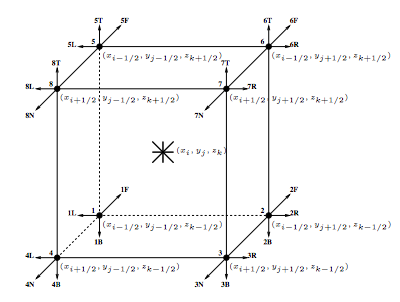
\includegraphics[width=0.6\linewidth]{figures/CartesianDiscretization.jpg}
\caption{Cartesian discretization to be used for the cell balance schemes.}
\label{fig:CartesianDiscretization}
\end{figure}

\subsubsubsection{Cell Balance Schemes}

Cell balance schemes point values for the solution \(\psi\) over a discretized spatial mesh. With the definitions in Eq. \eqref{eq:OmegaComponentsCartesian} switched around to be consistent with the Denovo manual, integrating Eq. \eqref{eq:SimpleTE} over the mesh cell shown in Fig. \ref{fig:CartesianDiscretization} gives:

\begin{equation}
\int_{x_{i-1/2}}^{x_{i+1/2}}dx\mu \frac{\partial \psi}{\partial x}+\int_{y_{j-1/2}}^{y_{j+1/2}}dy\eta \frac{\partial \psi}{\partial y}+\int_{z_{k-1/2}}^{z_{k+1/2}}dz\xi \frac{\partial \psi}{\partial z}+\Sigma_{t,ijk}{E}\psi_{ijk}(\vv{r},E)=S_{ijk}(E)
\end{equation}

where it has been assumed that \(\Sigma_t\) and \(S\) are constant over the cell, and are represented by their cell-centered values. In addition, the energy-dependence has been dropped, though the dependency could easily be re-introduced by simply carrying around the \((E, t)\) notation after each occurrence of \(\psi\). Without approximation, the integrals in the above reduce to:

\begin{equation}
\label{eq:DiscretizedCartesianTE}
\frac{\mu}{\Delta_i}(\psi_{i+1/2}-\psi_{i-1/2})+\frac{\eta}{\Delta_j}(\psi_{j+1/2}-\psi_{j-1/2})+\frac{\xi}{\Delta_k}(\psi_{k+1/2}-\psi_{k-1/2})+\Sigma_{t,ijk}\psi_{ijk}=S_{ijk}
\end{equation}

With this discretization method, there must be some way to relate the cell-centered value \(ijk\) to the face values. The different options we have for discretization are related to the choices we can make for how to relate these quantities. The Diamond Difference and Step Difference schemes choose the following relationship:

\begin{equation}
\label{eq:DifferencingRelationship}
\psi_{i\pm1/2}=\frac{2}{1\pm\alpha}\psi_{ijk}-\frac{1\mp\alpha}{1\pm\alpha}\bar{\psi}_{i\mp1/2}
\end{equation}

and likewise for the \(y\) and \(z\) directions. \(\bar{\psi}\) represents a known flux, and depending on whether a sweep is being performed in the positive-\(\mu\) direction (\(\bar{\psi}_{i-1/2}\) is known) or in the negative-\(\mu\) direction (\(\bar{\psi}_{i+1/2}\) is known), either the + or - option is selected in Eq. \eqref{eq:DifferencingRelationship}. The objective is to choose the correct relationship in Eq. \eqref{eq:DifferencingRelationship} such that the known quantities, or the incoming fluxes to each cell, can be used to compute the unknown quantities, or the outgoing fluxes for each cell, in a ``sweep'' over the spatial mesh. For example, for a sweep in the positive-\(\mu\) direction, we supposedly know \(\bar{\psi}_{i-1/2}\), so we would relate the cell-centered flux to the outgoing flux in the following way:

\begin{equation}
\begin{aligned}
\psi_{i+1/2}=\frac{2}{1+\alpha}\psi_{ijk}-\frac{1-\alpha}{1+\alpha}\bar{\psi}_{i-1/2}\quad\quad\mu >0\\
\psi_{ijk}=\frac{1}{2}\left\lbrack(1+\alpha)\psi_{i+1/2}+(1-\alpha)\bar{\psi}_{i-1/2}\right\rbrack\\
\end{aligned}
\end{equation}

Likewise, for a sweep in the negative-\(\mu\) direction, we supposedly know \(\bar{\psi}_{i+1/2}\), so we would relate the cell-centered flux to the outgoing flux in the following way:

\begin{equation}
\begin{aligned}
\psi_{i-1/2}=\frac{2}{1-\alpha}\psi_{ijk}-\frac{1+\alpha}{1-\alpha}\bar{\psi}_{i+1/2}\quad\quad\mu <0\\
\psi_{ijk}=\frac{1}{2}\left\lbrack(1+\alpha)\psi_{i+1/2}+(1-\alpha)\bar{\psi}_{i-1/2}\right\rbrack\\
\end{aligned}
\end{equation}

Note that both of these provide equivalent expressions, but the choice depends on the sweep direction. The differencing scheme in Eq. \eqref{eq:DifferencingRelationship} is a Crank-Nicolson method in space. Inserting Eq. \eqref{eq:DifferencingRelationship} into the discretized transport equation in Eq. \eqref{eq:SimpleTE} gives the following equation for the cell-centered flux in terms of known quantities:

\begin{equation}
\label{eq:psi_ijk}
\psi_{ijk}=\frac{S_{ijk}+\frac{2}{1\pm\alpha}\left(\frac{|\mu|}{\Delta_i}\bar{\psi}_{i\mp1/2}+\frac{|\eta|}{\Delta_j}\bar{\psi}_{j\mp1/2}\right)+\frac{|\xi|}{\Delta_k}\bar{\psi}_{k\mp1/2}}{\Sigma_{t,ijk}+\frac{2}{1\pm\alpha}\left(\frac{|\mu|}{\Delta_i}+\frac{|\eta|}{\Delta_j}+\frac{|\xi|}{\Delta_k}\right)}
\end{equation}

where it has been assumed that \(\alpha\) is selected to be the same in all directions. \(\alpha\) is a parameter used to tune the spatial discretization. Common choices for \(\alpha\) have their own names. The Diamond Difference method sets \(\alpha=0\). With this choice, the cell-centered flux is an average of the face fluxes. The Step Difference method, on the other hand, sets \(\alpha=\pm1\) such that the cell-centered flux is set equal to the incoming face flux (choose 1 or -1 accordingly so that Eq. \eqref{eq:DifferencingRelationship} provides an expression for \(\psi_{ijk}\) in terms of the known incoming face flux).The Diamond Difference method is second-order in space, while the Step Difference method is only first-order. 

In a ``transport sweep,'' computation begins at a boundary for which the boundary condition is known. At this boundary, the incoming fluxes are known. Then, Eq. \eqref{eq:psi_ijk} is used to solve for \(\psi_{ijk}\) using the incoming flux values. Once the cell-centered flux is known, Eq. \eqref{eq:DifferencingRelationship} can be used to compute the outgoing cell fluxes, which serve as the incoming flux values for the next mesh cell. This process is repeated until each cell has been computed. If there are no scattering, fission, or external sources in Eq. \eqref{eq:psi_ijk}, then only one transport sweep is required. However, if these sources are present, then at the end of each sweep, an updated \(S_{ijk}\) must be computed, and the sweep repeated until reaching convergence. 

If reflective boundary conditions are present, then begin from the side of the domain for which the conditions are known, and then upon reaching the reflective boundary, apply the reflective condition, then perform a sweep in the opposite direction (using the other stepping relations developed for \(\mu<0\) instead of \(\mu>0\)). This double sweep is then halted to perform updates to \(S_{ijk}\) and then repeated until reaching convergence. If reflective boundary conditions exist on both ends of the domain, then an initial guess for the incoming fluxes at the starting point must be made, and then each double sweep is again halted to perform updates to \(S_{ijk}\) until reaching convergence. 

The Diamond Difference method can produce negative fluxes, and the onset of negative fluxes is related to the mesh spacing \(\Delta_i\). 

\begin{tcolorbox}[breakable]
The onset of negative fluxes with the Diamond Difference method can be shown by solving the 1-D, no-source form of Eq. \eqref{eq:SimpleTE} and then applying the Diamond Difference differencing scheme.

\begin{equation}
\label{eq:Ex2}
\mu\frac{d\psi}{dx}+\Sigma_t\psi=0
\end{equation}

The analytical solution to this equation is:

\begin{equation}
\frac{d\psi}{\psi}=\frac{-\Sigma_t}{\mu}dx\quad\rightarrow\quad\int_{x_{i-1/2}}^{x_{i+1/2}}\frac{d\psi}{\psi}=\int_{x_{i-1/2}}^{x_{i+1/2}}\frac{-\Sigma_t}{\mu}dx
\end{equation}

Performing the integration:

\begin{equation}
\label{eq:124}
\ln{\left(\frac{\psi_{i+1/2}}{\psi_{i-1/2}}\right)}=\frac{-\Sigma_t}{\mu}\Delta_i\quad\rightarrow\quad\psi_{i+1/2}=\exp{\left(\frac{-\Sigma_t}{\mu}\Delta_i\right)}\psi_{i-1/2}
\end{equation}

Alternatively, the Diamond Difference method can be used to determine how \(\psi_{i+1/2}\) is related (numerically, instead of analytically) to \(\psi_{i-1/2}\). Using \(\alpha=0\) in Eq. \eqref{eq:DifferencingRelationship}:

\begin{equation}
\label{eq:122}
\psi_{ijk}=\frac{1}{2}\left(\psi_{i+1/2}+\psi_{i-1/2}\right)
\end{equation}

The numeric form of Eq. \eqref{eq:Ex2} can be obtained in a manner very similar to that in Eq. \eqref{eq:DiscretizedCartesianTE}:

\begin{equation}
\label{eq:123}
\frac{\mu}{\Delta_i}(\psi_{i+1/2}-\psi_{i-1/2})+\Sigma_{t,ijk}\psi_{ijk}=0
\end{equation}

Inserting Eq. \eqref{eq:122} into Eq. \eqref{eq:123} to eliminate \(\psi_{ijk}\) in order to obtain an expression similar to that in Eq. \eqref{eq:124} in terms of only \(\psi_{i+1/2}\) and \(\psi_{i-1/2}\):

\begin{equation}
\psi_{i+1/2}=\frac{1-\Sigma_{t,ijk}\Delta_i/2\mu}{1+\Sigma_{t,ijk}\Delta_i/2\mu}\psi_{i-1/2}
\end{equation}

From this expression, \(\psi_{i+1/2}\) can be negative if:

\begin{equation}
\Delta_i>\frac{2|\mu|}{\Sigma_{t,ijk}}
\end{equation}

By comparing this numerical expression with the analytic expression in Eq. \eqref{eq:124}, we see that the truncation error in the Diamond Difference method is that the numerical expression on the LHS below is used to approximate the exponential term on the RHS:

\begin{equation}
\label{eq:125}
\frac{1-\Sigma_{t,ijk}\Delta_i/2\mu}{1+\Sigma_{t,ijk}}\approx\exp{\left(\frac{-\Sigma_t}{\mu}\Delta_i\right)}
\end{equation}

To determine the order of the truncation error, the Taylor series of \(e^x=1+x+\mathscr{O}(x^2)\). So, for the exponential on the RHS, the Taylor series is:

\begin{equation}
\text{Taylor series of } \exp{\left(\frac{-\Sigma_t}{\mu}\Delta_i\right)}=1+\frac{-\Sigma_{t,ijk}}{\mu}\Delta_i+\mathscr{\Delta_i}^2
\end{equation}

The term in the numerator of the fraction on the LHS of Eq. \eqref{eq:125} is very similar to the Taylor series above, and hence we can see that the truncation error of the Diamond Difference method in this case is of \(\mathscr{O}(\Sigma_t\Delta_i/2|\mu|)^2\). 

\end{tcolorbox}

\subsubsection{Quadrature}

\subsubsubsection{Level-Symmetric Quadrature}
While there are many options for quadrature sets, the Level-Symmetric quadrature set is the set most often associated with the \(S_N\) method. With this set, there are \(N(N+2)\) angular directions per spatial location (N(N+2)/8 per octant). The Level-Symmetric quadrature set uses the same set of \(N/2\) positive values of direction cosines for each of the components of \(\hat{\Omega}\). Because this quadrature set is symmetric, no direction gets preferential treatment. Different quadrature sets could be used for different computations where it is expected for streaming to occur preferentially in some directions over others. 

Because of the symmetry constraints, not all of the choices for the quadrature points are independent, and in fact there is only one degree of freedom for each choice of quadrature set. A second constraint given by Eq. \eqref{eq:QuadratureNormalization} then narrows down the options for the quadrature set. With these two constraints, \(S_2\) quadrature is fixed, but for higher orders, there are several options remaining for the quadrature points. 

\subsubsubsection{\(LQ_N\) Quadrature}

With the same symmetry and normalization constraints as the Level-Symmetric quadrature set, the \(LQ_N\) quadrature set imposes the additional requirement that the quadrature set should correctly integrate as many Legendre polynomials as possible. 

\subsubsection{Spatial Discretization}

The \(S_N\) equations provide the framework to discretize the angular flux in angle, but the equations still must be discretized in space. In general, there are two different means to perform spatial discretization - cell balance methods, which preserve conservation of the solution, and finite element methods, which do not necessarily preserve conservation of the solution. In a single mesh cell, cell balance methods will provide a statement that is equivalent to conservation of neutrons, while finite element methods satisfy the governing equation in a weighted-integral sense. For simplicity, all of the spatial discretization schemes discussed here are applied to the simplified transport equation that neglects time dependence and assumes some angular discretization has already been applied to \(\psi\) such that it is independent of angle (in each of these equations):

\begin{equation}
\label{eq:SimpleTE}
\hat{\Omega}\cdot\nabla\psi(\vv{r},E)+\Sigma_t({\vv{r},E})\psi(\vv{r},E)=S(\vv{r},E)
\end{equation}

where \(S\) represents the scattering, fission, and external sources. There will be one of these equations for each discrete direction in the \(S_N\) method. For all the following discretization schemes, a Cartesian mesh given in Fig. \ref{fig:CartesianDiscretization} is assumed, with \(i\) representing indices in the \(x\)-direction, \(j\) in the \(y\)-direction, and \(k\) in the \(z\)-direction.

\begin{figure}[H]
\centering
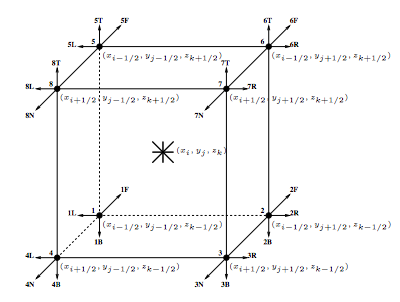
\includegraphics[width=0.6\linewidth]{figures/CartesianDiscretization.jpg}
\caption{Cartesian discretization to be used for the cell balance schemes.}
\label{fig:CartesianDiscretization}
\end{figure}

\subsubsubsection{Cell Balance Schemes}

Cell balance schemes point values for the solution \(\psi\) over a discretized spatial mesh. With the definitions in Eq. \eqref{eq:OmegaComponentsCartesian} switched around to be consistent with the Denovo manual, integrating Eq. \eqref{eq:SimpleTE} over the mesh cell shown in Fig. \ref{fig:CartesianDiscretization} gives:

\begin{equation}
\int_{x_{i-1/2}}^{x_{i+1/2}}dx\mu \frac{\partial \psi}{\partial x}+\int_{y_{j-1/2}}^{y_{j+1/2}}dy\eta \frac{\partial \psi}{\partial y}+\int_{z_{k-1/2}}^{z_{k+1/2}}dz\xi \frac{\partial \psi}{\partial z}+\Sigma_{t,ijk}{E}\psi_{ijk}(\vv{r},E)=S_{ijk}(E)
\end{equation}

where it has been assumed that \(\Sigma_t\) and \(S\) are constant over the cell, and are represented by their cell-centered values. In addition, the energy-dependence has been dropped, though the dependency could easily be re-introduced by simply carrying around the \((E, t)\) notation after each occurrence of \(\psi\). Without approximation, the integrals in the above reduce to:

\begin{equation}
\label{eq:DiscretizedCartesianTE}
\frac{\mu}{\Delta_i}(\psi_{i+1/2}-\psi_{i-1/2})+\frac{\eta}{\Delta_j}(\psi_{j+1/2}-\psi_{j-1/2})+\frac{\xi}{\Delta_k}(\psi_{k+1/2}-\psi_{k-1/2})+\Sigma_{t,ijk}\psi_{ijk}=S_{ijk}
\end{equation}

With this discretization method, there must be some way to relate the cell-centered value \(ijk\) to the face values. The different options we have for discretization are related to the choices we can make for how to relate these quantities. The Diamond Difference and Step Difference schemes choose the following relationship:

\begin{equation}
\label{eq:DifferencingRelationship}
\psi_{i\pm1/2}=\frac{2}{1\pm\alpha}\psi_{ijk}-\frac{1\mp\alpha}{1\pm\alpha}\bar{\psi}_{i\mp1/2}
\end{equation}

and likewise for the \(y\) and \(z\) directions. \(\bar{\psi}\) represents a known flux, and depending on whether a sweep is being performed in the positive-\(\mu\) direction (\(\bar{\psi}_{i-1/2}\) is known) or in the negative-\(\mu\) direction (\(\bar{\psi}_{i+1/2}\) is known), either the + or - option is selected in Eq. \eqref{eq:DifferencingRelationship}. The objective is to choose the correct relationship in Eq. \eqref{eq:DifferencingRelationship} such that the known quantities, or the incoming fluxes to each cell, can be used to compute the unknown quantities, or the outgoing fluxes for each cell, in a ``sweep'' over the spatial mesh. For example, for a sweep in the positive-\(\mu\) direction, we supposedly know \(\bar{\psi}_{i-1/2}\), so we would relate the cell-centered flux to the outgoing flux in the following way:

\begin{equation}
\begin{aligned}
\psi_{i+1/2}=\frac{2}{1+\alpha}\psi_{ijk}-\frac{1-\alpha}{1+\alpha}\bar{\psi}_{i-1/2}\quad\quad\mu >0\\
\psi_{ijk}=\frac{1}{2}\left\lbrack(1+\alpha)\psi_{i+1/2}+(1-\alpha)\bar{\psi}_{i-1/2}\right\rbrack\\
\end{aligned}
\end{equation}

Likewise, for a sweep in the negative-\(\mu\) direction, we supposedly know \(\bar{\psi}_{i+1/2}\), so we would relate the cell-centered flux to the outgoing flux in the following way:

\begin{equation}
\begin{aligned}
\psi_{i-1/2}=\frac{2}{1-\alpha}\psi_{ijk}-\frac{1+\alpha}{1-\alpha}\bar{\psi}_{i+1/2}\quad\quad\mu <0\\
\psi_{ijk}=\frac{1}{2}\left\lbrack(1+\alpha)\psi_{i+1/2}+(1-\alpha)\bar{\psi}_{i-1/2}\right\rbrack\\
\end{aligned}
\end{equation}

Note that both of these provide equivalent expressions, but the choice depends on the sweep direction. The differencing scheme in Eq. \eqref{eq:DifferencingRelationship} is a Crank-Nicolson method in space. Inserting Eq. \eqref{eq:DifferencingRelationship} into the discretized transport equation in Eq. \eqref{eq:SimpleTE} gives the following equation for the cell-centered flux in terms of known quantities:

\begin{equation}
\label{eq:psi_ijk}
\psi_{ijk}=\frac{S_{ijk}+\frac{2}{1\pm\alpha}\left(\frac{|\mu|}{\Delta_i}\bar{\psi}_{i\mp1/2}+\frac{|\eta|}{\Delta_j}\bar{\psi}_{j\mp1/2}+\frac{|\xi|}{\Delta_k}\bar{\psi}_{k\mp1/2}\right)}{\Sigma_{t,ijk}+\frac{2}{1\pm\alpha}\left(\frac{|\mu|}{\Delta_i}+\frac{|\eta|}{\Delta_j}+\frac{|\xi|}{\Delta_k}\right)}
\end{equation}

where it has been assumed that \(\alpha\) is selected to be the same in all directions. \(\alpha\) is a parameter used to tune the spatial discretization. Common choices for \(\alpha\) have their own names. The Diamond Difference method sets \(\alpha=0\). With this choice, the cell-centered flux is an average of the face fluxes. The Step Difference method, on the other hand, sets \(\alpha=\pm1\) such that the cell-centered flux is set equal to the incoming face flux (choose 1 or -1 accordingly so that Eq. \eqref{eq:DifferencingRelationship} provides an expression for \(\psi_{ijk}\) in terms of the known incoming face flux).The Diamond Difference method is second-order in space, while the Step Difference method is only first-order. 

In a ``transport sweep,'' computation begins at a boundary for which the boundary condition is known. At this boundary, the incoming fluxes are known. Then, Eq. \eqref{eq:psi_ijk} is used to solve for \(\psi_{ijk}\) using the incoming flux values. Once the cell-centered flux is known, Eq. \eqref{eq:DifferencingRelationship} can be used to compute the outgoing cell fluxes, which serve as the incoming flux values for the next mesh cell. This process is repeated until each cell has been computed. If there are no scattering, fission, or external sources in Eq. \eqref{eq:psi_ijk}, then only one transport sweep is required. However, if these sources are present, then at the end of each sweep, an updated \(S_{ijk}\) must be computed, and the sweep repeated until reaching convergence. 

If reflective boundary conditions are present, then begin from the side of the domain for which the conditions are known, and then upon reaching the reflective boundary, apply the reflective condition, then perform a sweep in the opposite direction (using the other stepping relations developed for \(\mu<0\) instead of \(\mu>0\)). This double sweep is then halted to perform updates to \(S_{ijk}\) and then repeated until reaching convergence. If reflective boundary conditions exist on both ends of the domain, then an initial guess for the incoming fluxes at the starting point must be made, and then each double sweep is again halted to perform updates to \(S_{ijk}\) until reaching convergence. 

The Diamond Difference method can produce negative fluxes, and the onset of negative fluxes is related to the mesh spacing \(\Delta_i\). Some codes have options called ``Negative-Flux-Fixup'' that remedy these negative fluxes in order to still use relatively coarse spatial meshes. In these methods, whenever an outgoing flux is computed to be negative, then the face flux is set to zero, and \(\psi_{ijk}\) recalculated. This is repeated until all outgoing fluxes are positive. Because the corrected solution depends on \(\psi\), this method is nonlinear.  

\begin{tcolorbox}[breakable]
The onset of negative fluxes with the Diamond Difference method can be shown by solving the 1-D, no-source form of Eq. \eqref{eq:SimpleTE} and then applying the Diamond Difference differencing scheme.

\begin{equation}
\label{eq:Ex2}
\mu\frac{d\psi}{dx}+\Sigma_t\psi=0
\end{equation}

The analytical solution to this equation is:

\begin{equation}
\frac{d\psi}{\psi}=\frac{-\Sigma_t}{\mu}dx\quad\rightarrow\quad\int_{x_{i-1/2}}^{x_{i+1/2}}\frac{d\psi}{\psi}=\int_{x_{i-1/2}}^{x_{i+1/2}}\frac{-\Sigma_t}{\mu}dx
\end{equation}

Performing the integration:

\begin{equation}
\label{eq:124}
\ln{\left(\frac{\psi_{i+1/2}}{\psi_{i-1/2}}\right)}=\frac{-\Sigma_t}{\mu}\Delta_i\quad\rightarrow\quad\psi_{i+1/2}=\exp{\left(\frac{-\Sigma_t}{\mu}\Delta_i\right)}\psi_{i-1/2}
\end{equation}

Alternatively, the Diamond Difference method can be used to determine how \(\psi_{i+1/2}\) is related (numerically, instead of analytically) to \(\psi_{i-1/2}\). Using \(\alpha=0\) in Eq. \eqref{eq:DifferencingRelationship}:

\begin{equation}
\label{eq:122}
\psi_{ijk}=\frac{1}{2}\left(\psi_{i+1/2}+\psi_{i-1/2}\right)
\end{equation}

The numeric form of Eq. \eqref{eq:Ex2} can be obtained in a manner very similar to that in Eq. \eqref{eq:DiscretizedCartesianTE}:

\begin{equation}
\label{eq:123}
\frac{\mu}{\Delta_i}(\psi_{i+1/2}-\psi_{i-1/2})+\Sigma_{t,ijk}\psi_{ijk}=0
\end{equation}

Inserting Eq. \eqref{eq:122} into Eq. \eqref{eq:123} to eliminate \(\psi_{ijk}\) in order to obtain an expression similar to that in Eq. \eqref{eq:124} in terms of only \(\psi_{i+1/2}\) and \(\psi_{i-1/2}\):

\begin{equation}
\psi_{i+1/2}=\frac{1-\Sigma_{t,ijk}\Delta_i/2\mu}{1+\Sigma_{t,ijk}\Delta_i/2\mu}\psi_{i-1/2}
\end{equation}

From this expression, \(\psi_{i+1/2}\) can be negative if:

\begin{equation}
\Delta_i>\frac{2|\mu|}{\Sigma_{t,ijk}}
\end{equation}

By comparing this numerical expression with the analytic expression in Eq. \eqref{eq:124}, we see that the truncation error in the Diamond Difference method is that the numerical expression on the LHS below is used to approximate the exponential term on the RHS:

\begin{equation}
\label{eq:125}
\frac{1-\Sigma_{t,ijk}\Delta_i/2\mu}{1+\Sigma_{t,ijk}}\approx\exp{\left(\frac{-\Sigma_t}{\mu}\Delta_i\right)}
\end{equation}

To determine the order of the truncation error, the Taylor series of \(e^x=1+x+\mathscr{O}(x^2)\). So, for the exponential on the RHS, the Taylor series is:

\begin{equation}
\text{Taylor series of } \exp{\left(\frac{-\Sigma_t}{\mu}\Delta_i\right)}=1+\frac{-\Sigma_{t,ijk}}{\mu}\Delta_i+\mathscr{O}(\Delta_i)^2
\end{equation}

The term in the numerator of the fraction on the LHS of Eq. \eqref{eq:125} is very similar to the Taylor series above, and hence we can see that the truncation error of the Diamond Difference method in this case is of \(\mathscr{O}(\Sigma_t\Delta_i/2|\mu|)^2\). 
\end{tcolorbox}

Aside from the Diamond Difference and Step Difference schemes, a third differencing scheme, Theta-Weighted Diamond Difference, chooses two additional weight parameters based on the incoming fluxes. These additional parameters allow the outgoing fluxes to vary smoothly between the Step and Diamond Difference schemes. These weighting parameters are bounded between the Diamond Difference and Step Difference methods. Provided the source is positive, the Theta-Weighted Diamond Difference and Weighted Diamond Difference with Flux-Fixup both give positive fluxes.

\subsubsection{Operator Form}

This section covers the operator form of the transport equation, where the scattering term has been expanded in spherical harmonics as in Eq. \eqref{eq:SnGeneral}, repeated below for convenience:

\begin{equation}
\label{eq:StartofOperatorForm}
\begin{aligned}
 \hat{\Omega}_a\cdot\nabla\psi_a^g(\vv{r}) + 
 \Sigma_t^g(\vv{r})\psi_a^g(\vv{r}) = \\
\sum_{l=0}^{N}\left\lbrack Y_{l0}^e(\hat{\Omega}_a)s_{l0}^g(\vv{r})+\sum_{m=1}^{l}\left(Y_{lm}^e(\hat{\Omega}_a)s_{lm}^g(\vv{r})+Y_{lm}^o(\hat{\Omega}_a)v_{lm}^g(\vv{r})\right)\right\rbrack+\\
\sum_{g'=1}^G\sum_{l=0}^{N}\Sigma_{s,l}(\vv{r}, g'\rightarrow g)\left\lbrack Y_{l0}^e(\hat{\Omega}_a)e_{l0}^{g'}(\vv{r})+\sum_{m=1}^{l}\left(Y_{lm}^e(\hat{\Omega}_a)e_{lm}^{g'}(\vv{r})+Y_{lm}^o(\hat{\Omega}_a)o_{lm}^{g'}(\vv{r})\right)\right\rbrack\quad\\
\end{aligned}
\end{equation}

where the equation has now been transformed to a form that accounts for energy groups, rather than applying to a within-group equation. So, all energy dependence is removed, since a group structure now accounts for that dependence. The \(g\) superscript refers to the energy group number, and \(G\) to the total number of energy groups. Within-group scattering is counted in the scattering term, but is canceled by the total interaction term, which avoids double counting. The above equation can be cast in operator form. The external group source is defined as:

\begin{equation}
q_e^g(\vv{r})=\sum_{l=0}^{N}\left\lbrack Y_{l0}^e(\hat{\Omega}_a)s_{l0}^g(\vv{r})+\sum_{m=1}^{l}\left(Y_{lm}^e(\hat{\Omega}_a)s_{lm}^g(\vv{r})+Y_{lm}^o(\hat{\Omega}_a)v_{lm}^g(\vv{r})\right)\right\rbrack
\end{equation}

in order to permit easier equation manipulation. In addition, several operators are defined. The transport operator is:

\begin{equation}
\textbf{L}\equiv\hat{\Omega}_a\cdot\nabla+\Sigma_t^g
\end{equation}

and the solution vector \(\Psi\) is a column vector containing each energy group flux vector \(\vv{\psi}\):

\begin{equation}
\Psi=\begin{bmatrix}\vv{\psi}_1&\vv{\psi}_2&\vv{\psi}_3&\cdots&\vv{\psi}_G\end{bmatrix}^T
\end{equation}

where \(\vv{\psi}\) is then a column vector that contains the flux for each discrete angle for that particular energy group \(g\):

\begin{equation}
\vv{\psi}_g=\begin{bmatrix}\psi_1^g&\psi_2^g&\psi_3^g&\cdots&\psi_n^g\end{bmatrix}^T
\end{equation}

So, the vector of unknowns is organized by energy group, and in the section pertaining to each group, by angle. In order to discuss the size of these matrices and vectors, several variables are defined:

\begin{equation}
\begin{aligned}
G=&\ \text{number of energy groups}\\
t = &\ \text{number of moments}\\
n = &\ \text{number of angles}\\
N = &\ P_N\text{\ order}\\
N_c=&\ \text{number of cells}\\
N_e=&\ \text{number of unknowns per cell}\\
\end{aligned}
\end{equation} 

So, if the problem consisted of a single cell with a single node (i.e. only one spatial unknown), then \(\Psi\) would be an \((Gn)\times1\) vector. However, the problems solves will consist of a spatial domain that is also present in \(\Psi\). In reality, each \(\psi_{\hat{\Omega}_n}^g\) term is solved as a function of space, and is therefore not a scalar value, but an \(N_cN_e\times1\) vector. The \(S_N\) equation for a particular angle and group is solved as a function of space using a variety of methods, such as the finite element method or the finite difference method. So, the total size of \(\Psi\) is \(N_cN_eGn\times1\). The external source \(q_e^g\) is defined in a similar manner, and is represented as \(Q\), an \(N_cN_eGn\times1\) vector.

Expressing the mapping between flux moments and the scattering term is more difficult simply due to the difficulty in visualizing the matrix multiplication. The moment-to-discrete matrix is used to project harmonic moments onto discrete angle space. It is defined as:

\begin{equation}
\textbf{M}=\left\{
\begin{array}{*{13}c}
Y_{00}^o(\hat{\Omega}_1) & Y_{00}^e(\hat{\Omega}_1) & Y_{01}^o(\hat{\Omega}_1) & Y_{01}^e(\hat{\Omega}_1) & Y_{10}^o(\hat{\Omega}_1) & Y_{10}^e(\hat{\Omega}_1) & Y_{11}^o(\hat{\Omega}_1) & Y_{11}^e(\hat{\Omega}_1) & \cdots & Y_{NN}^o(\hat{\Omega}_1) & Y_{NN}^e(\hat{\Omega}_1)\\
Y_{00}^o(\hat{\Omega}_2) & Y_{00}^e(\hat{\Omega}_2) & Y_{01}^o(\hat{\Omega}_2) & Y_{01}^e(\hat{\Omega}_2) & Y_{10}^o(\hat{\Omega}_2) & Y_{10}^e(\hat{\Omega}_2) & Y_{11}^o(\hat{\Omega}_2) & Y_{11}^e(\hat{\Omega}_2) & \cdots & Y_{NN}^o(\hat{\Omega}_2) & Y_{NN}^e(\hat{\Omega}_2)\\
\vdots & \vdots & \vdots & \vdots & \vdots & \vdots & \vdots & \vdots & \vdots & \vdots & \vdots \\
Y_{00}^o(\hat{\Omega}_n) & Y_{00}^e(\hat{\Omega}_n) & Y_{01}^o(\hat{\Omega}_n) & Y_{01}^e(\hat{\Omega}_n) & Y_{10}^o(\hat{\Omega}_n) & Y_{10}^e(\hat{\Omega}_n) & Y_{11}^o(\hat{\Omega}_n) & Y_{11}^e(\hat{\Omega}_n) & \cdots & Y_{NN}^o(\hat{\Omega}_n) & Y_{NN}^e(\hat{\Omega}_n)\\
\end{array}\right\}
\end{equation}

But, some of these components are actually always zero - for instance, from the expansion in Eq. \eqref{eq:StartofOperatorForm}, if \(l=0\), then there are no spherical harmonics for which \(m\neq0\). This eliminates \(Y_{01}^e\) and \(Y_{01}^o\). In addition, \(Y_{00}^o=0\) and \(Y_{10}^o=0\) since there is no odd component for \(l=0,i\) and \(m=0\). This gives a simplified version of the moment-to-discrete matrix, where the only difference between this matrix and the more explicit one above is that several of the low \(l\) and \(m\) spherical harmonics that are zero are removed.

\begin{equation}
\textbf{M}=\left\{
\begin{array}{*{13}c}
Y_{00}^e(\hat{\Omega}_1)  & Y_{10}^e(\hat{\Omega}_1) & Y_{11}^o(\hat{\Omega}_1) & Y_{11}^e(\hat{\Omega}_1) & Y_{20}^e(\hat{\Omega}_1) & \cdots & Y_{NN}^o(\hat{\Omega}_1) & Y_{NN}^e(\hat{\Omega}_1)\\
Y_{00}^e(\hat{\Omega}_2)  & Y_{10}^e(\hat{\Omega}_2) & Y_{11}^o(\hat{\Omega}_2) & Y_{11}^e(\hat{\Omega}_2) & Y_{20}^e(\hat{\Omega}_2) & \cdots & Y_{NN}^o(\hat{\Omega}_2) & Y_{NN}^e(\hat{\Omega}_2)\\
\vdots & \vdots & \vdots & \vdots & \vdots & \vdots & \vdots & \vdots \\
Y_{00}^e(\hat{\Omega}_n) & Y_{10}^e(\hat{\Omega}_n) & Y_{11}^o(\hat{\Omega}_n) & Y_{11}^e(\hat{\Omega}_n) & Y_{20}^e(\hat{\Omega}_n) & \cdots & Y_{NN}^o(\hat{\Omega}_n) & Y_{NN}^e(\hat{\Omega}_n)\\
\end{array}\right\}
\end{equation}

The scattering matrix contains along its diagonal the scattering moments:

\begin{equation}
\textbf{S}_{g^{'}\rightarrow g}=\begin{bmatrix}
\Sigma_{s0}
\end{bmatrix}
\end{equation}

With this definition, the discretization of the transport equation leads to the following matrix system:

\begin{equation}
\textbf{L}\begin{bmatrix}\Psi_1\\\Psi_2\\\Psi_3\\\vdots\\\Psi_G\end{bmatrix}=
\begin{bmatrix}
\textbf{M} & 0 & 0 & 0 & 0\\
0 & \textbf{M} & 0 & 0 & 0\\
0 & 0 & \textbf{M} & 0 & 0\\
0 & 0 & 0 & \cdots & 0\\
0 & 0 & 0 & 0 & \textbf{M}\\
\end{bmatrix}
\begin{bmatrix}
\textbf{S}_{11} & \textbf{S}_{12} & \textbf{S}_{13} & \cdots & \textbf{S}_{1G}\\
\textbf{S}_{21} & \textbf{S}_{22} & \textbf{S}_{23} & \cdots & \textbf{S}_{2G}\\
\textbf{S}_{31} & \textbf{S}_{32} & \textbf{S}_{33} & \cdots & \textbf{S}_{3G}\\
\vdots & \vdots & \vdots & \vdots & \vdots\\
\textbf{S}_{G1} & \textbf{S}_{G2} & \textbf{G}_{23} & \cdots & \textbf{S}_{GG}\\
\end{bmatrix}
\begin{bmatrix}
\Phi_1\\\Phi_2\\\Phi_3\\\vdots\\\Phi_G
\end{bmatrix}
+
\begin{bmatrix}
Q_1\\Q_2\\Q_3\\\vdots\\Q_G
\end{bmatrix}
\end{equation}

Hence, the upper triangular portion of the scattering matrix represents upscattering, while the diagonal represents within-group scattering, and the lower triangular portion represents downscattering. \(\Phi\) represents a vector of the angular flux moments used in the expansion of the scattering term, organized by group. 

\begin{equation}
\Phi_g=\begin{bmatrix}
o_{00}^g & e_{00}^g & o_{01}^g & e_{01}^g & o_{10}^g & e_{10}^g & \cdots & o_{NN}^g & e_{NN}^g\\
\end{bmatrix}^T
\end{equation}

where \(e_{lm}\) and \(o_{lm}\) are defined by Eq. \eqref{eq:FluxMoments31}. Note, however, that some of these terms are zero due to how the expansion is performed. Moments with \(l=0\) are only nonzero for \(m=0\). And, there is no odd component for \(l=0\). 

\begin{equation}
\Phi_g=\begin{bmatrix}
e_{00}^g & e_{10}^g & o_{11}^g & e_{11}^g & \cdots & o_{NN}^g & e_{NN}^g\\
\end{bmatrix}^T
\end{equation}

The flux moment vector can be related to the angular flux vector by \(\textbf{D}\):



\section{Spectral Angular Methods}
An alternative to the \(S_N\) method is to expand the angular dependence in a set of functions. In general 3-D geometries, we choose these functions to be the spherical harmonics functions. In 1-D, the spherical harmonics reduce to Legendre polynomials. 


\subsection{Spherical Harmonics \(P_N\)}

Instead of discretizing in angle as with the \(S_N\) method, we can expand the flux in the spherical harmonics to approximate the angular dependence. The accuracy of this method depends on how strongly \(\psi\) is a function of angle. This method, called the \(P_N\) method, can produce equations in higher dimensions, but is easiest to derive in 1-D Cartesian geometry because then the spherical harmonics reduce to the Legendre polynomials. This method provides reasonably-correct spatial solutions, but errors are often present in magnitude, which can be difficult to detect.

\subsubsection{1-D Cartesian Derivation}

Due to the added complexity associated with higher dimensions, the \(P_N\) equations are derived here for the time-independent form of the 1-D, monoenergetic transport equation in Cartesian geometries given by Eq. \eqref{eq:TE_Cartesian_1D_2_noenergy}, repeated here for reference, where the external and fission source are bundled together into \(S\), which is assumed isotropic:

\begin{equation*}
\mu \frac{\partial \psi(z, \mu)}{\partial z} +
 \Sigma_t(z)\psi(z, \mu) =\int_{4\pi}^{} d\hat{\Omega}' \Sigma_s(z, \hat{\Omega}\cdot\hat{\Omega}')\psi(z,\hat{\Omega}') + \frac{S(z)}{4\pi}
 \end{equation*}

The \(P_N\) approximation is made by expanding both the flux and scattering cross section in Legendre polynomials in a similar fashion to the scattering cross section as shown in Eq. \eqref{eq:ScatteringLegendre}. We use Legendre polynomials here because we're in 1-D Cartesian geometry; in higher dimensions or in non-Cartesian frames, the spherical harmonics would be needed.

\begin{equation}
\label{eq:AngularFluxPN}
\psi(z,\mu)=\sum_{n=0}^{\infty}\frac{2n+1}{4\pi}\phi_n(z)P_n(\mu)
\end{equation}

\begin{equation}
\label{eq:PNScatteringCrossSectionExpansion}
\Sigma_s(z,\hat{\Omega}\cdot\hat{\Omega}')=\sum_{l=0}^{\infty}\frac{2l+1}{4\pi}\Sigma_{sl}(z)P_l(\hat{\Omega}\cdot\hat{\Omega}')\rightarrow\sum_{l=0}^{\infty}\frac{2l+1}{4\pi}\Sigma_{sl}(z)P_l(\mu)P_l(\mu')
\end{equation}

where \(n\) is used in the expansion of the flux to differentiate it from \(l\) used in expanding the scattering cross section. From the 1-D form of the addition theorem for spherical harmonics given in Eq. \eqref{eq:AddSpherical1D}, the scattering cross section expansion has been simplified. Now, inserting Eqs. \eqref{eq:AngularFluxPN} and \eqref{eq:AngularFluxPN} into the 1-D transport equation listed in the beginning of this section:

\begin{equation}
\begin{aligned}
\mu \frac{\partial}{\partial z}\left(\sum_{n=0}^{\infty}\frac{2n+1}{4\pi}\phi_n(z)P_n(\mu)\right) + \Sigma_t(z)\sum_{n=0}^{\infty}\frac{2n+1}{4\pi}\phi_n(z)P_n(\mu) =\quad\quad\\
\int_{4\pi}^{} d\hat{\Omega}' \sum_{l=0}^{\infty}\frac{2l+1}{4\pi}\Sigma_{sl}(z)P_l(\mu)P_l(\mu')\sum_{n=0}^{\infty}\frac{2n+1}{4\pi}\phi_n(z)P_n(\mu) + \frac{S(z)}{4\pi}
 \end{aligned}
 \end{equation}

Because no quantities depend on \(\hat{\Omega}\), the scattering integral can be integrated over \(0\leq\phi\leq2\pi\) so that the integral becomes a function of only \(\mu\) and space.

\begin{equation}
\label{eq:PNStep1}
\begin{aligned}
\mu \frac{\partial}{\partial z}\left(\sum_{n=0}^{\infty}\frac{2n+1}{4\pi}\phi_n(z)P_n(\mu)\right) + \Sigma_t(z)\sum_{n=0}^{\infty}\frac{2n+1}{4\pi}\phi_n(z)P_n(\mu) =\quad\quad\\
2\pi\int_{-1}^{1} d\mu' \sum_{l=0}^{\infty}\frac{2l+1}{4\pi}\Sigma_{sl}(z)P_l(\mu)P_l(\mu')\sum_{n=0}^{\infty}\frac{2n+1}{4\pi}\phi_n(z)P_n(\mu) + \frac{S(z)}{4\pi}
 \end{aligned}
 \end{equation}
 
The orthogonality property of Legendre polynomials given in Eq. \eqref{eqn:LegendrePolynomialsOrthogonality} does not permit any extra terms (that depend on \(\mu\)) to be present in the integrand. Hence, the first term in Eq. \eqref{eq:PNStep1} must be rewritten using the recursive property of Legendre polynomials given in Eq. \eqref{eqn:LegendrePolynomialRecursion1}:

 \begin{equation}
\label{eq:PNStep2}
\begin{aligned}
\frac{\partial}{\partial z}\left(\sum_{n=0}^{\infty}\frac{\cancel{2n+1}}{4\pi}\phi_n(z)\frac{1}{\cancel{2n+1}} \left\lbrack(n+1)P_{n+1}(\mu) + n P_{n-1}(\mu)\right\rbrack\right) + \Sigma_t(z)\sum_{n=0}^{\infty}\frac{2n+1}{4\pi}\phi_n(z)P_n(\mu) =\quad\quad\\
2\pi\int_{-1}^{1} d\mu' \sum_{l=0}^{\infty}\frac{2l+1}{4\pi}\Sigma_{sl}(z)P_l(\mu)P_l(\mu')\sum_{n=0}^{\infty}\frac{2n+1}{4\pi}\phi_n(z)P_n(\mu) + \frac{S(z)}{4\pi}
 \end{aligned}
 \end{equation}
 
 Multiplying Eq. \eqref{eq:PNStep2} by \(P_n(\mu)\) and then integrating over \(-1\leq\mu\leq1\) gives, after canceling the \(1/4\pi\) from each term:
 
  \begin{equation}
\label{eq:PNStep3}
\begin{aligned}
\frac{\partial}{\partial z}\left(\sum_{n=0}^{\infty}\left\lbrack\int_{-1}^{1}d\mu\phi_n(z)(n+1)P_{n+1}(\mu)P_n(\mu) + \int_{-1}^{1}d\mu\phi_n(z)n P_{n-1}(\mu)P_n(\mu)\right\rbrack\right) + \quad\quad\\
\Sigma_t(z)\sum_{n=0}^{\infty}(2n+1)\int_{-1}^{1}d\mu\phi_n(z)P_n(\mu)P_n(\mu) =\quad\quad\\
\int_{-1}^{1}d\mu P_n(\mu)2\pi\int_{-1}^{1} d\mu' \sum_{l=0}^{\infty}\frac{2l+1}{4\pi}\Sigma_{sl}(z)P_l(\mu)P_l(\mu')\sum_{n=0}^{\infty}(2n+1)\phi_n(z)P_n(\mu)P_n(\mu) + \int_{-1}^{1}d\mu S(z)P_n(\mu)
 \end{aligned}
 \end{equation}

Then, applying the orthogonality property of Legendre polynomials from Eq. \eqref{eqn:LegendrePolynomialsOrthogonality} gives:

  \begin{equation}
\label{eq:PNStep4}
\begin{aligned}
\frac{\partial}{\partial z}\left(\sum_{n=0}^{\infty}\left\lbrack\frac{2(n+1)}{2n+1}\phi_{n+1}(z) +\frac{2n}{2n+1} \phi_{n-1}(z)\right\rbrack\right) + \Sigma_t(z)\sum_{n=0}^{\infty}2\phi_n(z) =\quad\quad\\
2\sum_{l=0}^{\infty}\Sigma_{sl}(z)\sum_{n=0}^{\infty}\phi_n(z) + \int_{-1}^{1}d\mu S(z)P_n(\mu)
 \end{aligned}
 \end{equation}

where orthogonality was applied twice to the scattering term. Dividing through by 2 then gives the \(P_N\) equations for 1-D Cartesian geometries:

\begin{equation}
\label{eq:PNStep5}
\begin{aligned}
\frac{\partial}{\partial z}\left(\sum_{n=0}^{\infty}\left\lbrack\frac{n+1}{2n+1}\phi_{n+1}(z) +\frac{n}{2n+1} \phi_{n-1}(z)\right\rbrack\right) + \Sigma_t(z)\sum_{n=0}^{\infty}\phi_n(z) =\quad\quad\\
\sum_{l=0}^{\infty}\Sigma_{sl}(z)\sum_{n=0}^{\infty}\phi_n(z) + \delta_{n,even}\frac{1}{2}\int_{-1}^{1}d\mu S(z)P_n(\mu)
 \end{aligned}
 \end{equation}

Because \(S(z)\) is not a function of \(\mu\), then the integral of a Legendre polynomial over its basis will give zero if that Legendre polynomial is an odd function, and will be nonzero otherwise. Hence, the source term is only present for even \(n\), based on the first few Legendre polynomials shown in Eq. \eqref{eqn:LegendrePolynomials_P0P1P2}. Now, in order to make this solution method tractable, the infinite sums have to be truncated at some point. It is also customary to set \(l=n\) such that the above reduce to:

\begin{equation}
\label{eq:PNStep6}
\begin{aligned}
\frac{\partial}{\partial z}\left(\sum_{n=0}^{N}\left\lbrack\frac{n+1}{2n+1}\phi_{n+1}(z) +\frac{n}{2n+1} \phi_{n-1}(z)\right\rbrack\right) + \Sigma_t(z)\sum_{n=0}^{N}\phi_n(z) =\quad\quad\\
\sum_{n=0}^{N}\Sigma_{sn}(z)\phi_n(z) +  \delta_{n,even}\frac{1}{2}\int_{-1}^{1}d\mu S(z)P_n(\mu)
 \end{aligned}
 \end{equation}

We can require Eq. \eqref{eq:PNStep6} to hold for all \(N\) at once, but we can also require it to hold for each \(N\). This stricter requirement returns the requirement stated in Eq. \eqref{eq:PNStep6}, and hence the \(P_N\) equations in practice produce \(N\) coupled ODEs:

\begin{equation}
\label{eq:PNEquations}
\begin{aligned}
\frac{\partial}{\partial z}\left\lbrack\frac{n+1}{2n+1}\phi_{n+1}(z) +\frac{n}{2n+1} \phi_{n-1}(z)\right\rbrack + \Sigma_t(z)\phi_n(z) =
\Sigma_{sn}(z)\phi_n(z) +  \delta_{n,even}\frac{1}{2}\int_{-1}^{1}d\mu S(z)P_n(\mu)
 \end{aligned}
 \end{equation}

This gives \(N+1\) coupled equations. For example, some of the first \(P_N\) equations are:
 
 \begin{equation}
 \begin{aligned}
\frac{\partial\phi_{1}(z)}{\partial z} + \Sigma_t(z)\phi_0(z)=\Sigma_{s0}\phi_0(z)+ S_0(z)\quad\quad n=0\\
\frac{2}{3}\frac{\partial\phi_{2}(z)}{\partial z}+\frac{1}{3}\frac{\partial\phi_{0}(z)}{\partial z} + \Sigma_t(z)\phi_1(z)=\Sigma_{s1}\phi_1(z)\quad\quad n=1\\
\frac{3}{5}\frac{\partial\phi_{3}(z)}{\partial z}+\frac{2}{5}\frac{\partial\phi_{1}(z)}{\partial z} + \Sigma_t(z)\phi_2(z)=\Sigma_{s2}\phi_2(z)+ S_2(z)\quad\quad n=2\\
\end{aligned}
\end{equation}

In order to truncate the infinite series to \(N\) unknowns, \(\phi_{-1}=0\) is often set, and either \(\phi_{N+1}=0\) or \(\partial\phi_{N+1}/\partial z=0\) is set as the other condition, where both give equivalent results. \(N\) is usually selected to be odd. If \(N\) were even, then artificial symmetry would be introduced into the problem through application of boundary conditions. In addition, for even \(N\), you do not obtain any additional information (non-linearly independent) from the \(P_N\) equations. 

\subsubsubsection{Boundary Conditions}
Marshak boundary conditions require continuity in the odd flux moments at boundaries. 

\begin{equation}
2\pi\int_{\hat{\Omega}\cdot\hat{n}<0}^{}d\mu P_l(\mu)\psi(\mu)=2\mu\int_{\hat{\Omega}\cdot\hat{n}<0}^{}d\mu P_l(\mu)\psi_b(\mu)\quad\quad l=1, 3, 5\cdots N
\end{equation}

where \(\psi_b(\mu)\) is the incoming flux. Expanding flux according to Eq. \eqref{eq:AngularFluxPN} gives:

\begin{equation}
2\pi\int_{\hat{\Omega}\cdot\hat{n}<0}^{}d\mu P_l(\mu)\sum_{n=0}^{\infty}\frac{2n+1}{4\pi}\phi_n(z)P_n(\mu)=2\mu\int_{\hat{\Omega}\cdot\hat{n}<0}^{}d\mu P_l(\mu)\psi_b(\mu)\quad\quad l=1, 3, 5\cdots N
\end{equation}

This gives \((N+1)/2\) boundary conditions. For an isotropic boundary:

\begin{equation}
\psi_b(\mu)=\frac{\phi_b}{4\pi}
\end{equation}

For a reflecting boundary, the net current at that boundary is zero. From the form of Eq. \eqref{eq:ScatteringMomentsLegendre}, it can be seen that the flux moments are given by:

\begin{equation}
\phi_l(z)=2\pi\int_{-1}^{1}d\mu\psi(\mu)P_l(\mu)
\end{equation}

For \(l=1\), we see that \(\phi_1\) represents the current. Hence, reflecting boundary conditions extend this argument to require that on vacuum boundaries:

\begin{equation}
\phi_l=0\quad\quad l=1, 3, 5, \cdots, N
\end{equation}

\subsection{Simplified Spherical Harmonics \(SP_N\)}
\label{sec:SPN}

The \(SP_N\), or Simplified \(P_N\), method was developed by Ely Gelbard in the early 1960s as an extension of the 1-D Cartesian \(P_N\) equations to higher dimensions. The \(SP_N\) method represents a``middle-ground'' between the full transport equation and diffusion theory. Gelbard ``derived'' the \(SP_N\) equations by extending the 1-D \(P_N\) equations to 3-D, with relatively little mathematical basis. The \(SP_N\) equations are equivalent to the \(P_N\) equations in slab geometries and in other limited cases, and it is only the relatively good numerical results that justified the use of the method initially, since it was not derived in a particularly rigorous manner. It was not until the 1990s that several mathematicians demonstrated that the \(SP_N\) method does have mathematical foundation, and it was shown that the \(SP_N\) equations are an asymptotic approximation to the transport equation. 

The \(SP_N\) method does not always give superior results to diffusion theory, and if the system is not diffusive or not locally 1-D, then the method gives poorer answers than diffusion theory. Away from the asymptotic limit to the transport equation, the \(SP_N\) equations break down. 

However, the \(SP_N\) equations contain more transport physics than the diffusion equation, and hence can be used to capture boundary layers that would be missed by diffusion theory. With the \(P_N\) equations, in the limit of \(N\rightarrow\infty\), the \(P_N\) solutions converge to the true solution, while this is not necessarily the case with the \(SP_N\) equations. Because the \(SP_N\) equations require higher computational cost, the best intermediate choice is to use the \(SP_3\) equations, since these offer much better solutions than the diffusion equation, without exceptionally higher cost.

A heuristic derivation of the \(SP_N\) equations can be performed using simple arguments regarding the form of the 1-D \(P_N\) equations in Eq. \eqref{eq:PNEquations}. The key to deriving the \(SP_N\) equations is to transform Eq. \eqref{eq:PNEquations} such that the derivative in the even-\(n\) equations is replaced by a divergence, while the derivative in the odd-\(n\) equations is replaced by a gradient. The \(SP_N\) equations therefore are:

\begin{equation}
\label{eq:SPNEquations}
\begin{aligned}
\frac{n+1}{2n+1}\nabla\cdot\vv{\phi}_{n+1}(z)+\frac{n}{2n+1}\nabla\cdot\vv{\phi}_{n-1}(z)+ \Sigma_t(z)\phi_n(z)=\Sigma_{sn}\phi_n(z)+ S_n(z)\quad \textrm{even - } n\\
\frac{n+1}{2n+1}\nabla\phi_{n+1}(z)+\frac{n}{2n+1}\nabla\phi_{n-1}(z)+ \Sigma_t(z)\vv{\phi}_n(z)=\Sigma_{sn}\vv{\phi}_n(z)\quad \textrm{odd - } n\\
\end{aligned}
 \end{equation}

This first-order form gives \(N+1\) equations. The \(SP_N\) equations can also be written in second-order form by solving for the odd moments in the odd-\(n\) equations, and then substituting this into the even moment equations. From the odd-\(n\) equation in Eq. \eqref{eq:SPNEquations}, we obtain:

\begin{equation}
\vv{\phi}_n(z)=\frac{1}{\Sigma_t(z)-\Sigma_{sn}(z)}\left(\frac{n+1}{2n+1}\nabla\phi_{n+1}(z)+\frac{n}{2n+1}\nabla\phi_{n-1}(z)\right)
\end{equation}

because \(\phi_{n+1}\) and \(\phi_n-1\) appear in the \(SP_N\) equations, the above can be used to determine the following additional relationships:

\begin{equation}
\begin{aligned}
\vv{\phi}_{n-1}(z)=\frac{1}{\Sigma_t(z)-\Sigma_{s,n-1}(z)}\left(\frac{n}{2n-1}\nabla\phi_{n}(z)+\frac{n-1}{2n-1}\nabla\phi_{n-2}(z)\right)\\
\vv{\phi}_{n+1}(z)=\frac{1}{\Sigma_t(z)-\Sigma_{s,n+1}(z)}\left(\frac{n+2}{2n+3}\nabla\phi_{n+2}(z)+\frac{n+1}{2n+3}\nabla\phi_{n}(z)\right)\\
\end{aligned}
\end{equation}

Inserting these expressions into the first-order form of the \(SP_N\) equations Eq. \eqref{eq:SPNEquations} then gives the second-order form, which holds for even \(n\):

\begin{equation}
\label{eq:SPNEquations}
\begin{aligned}
\frac{n+1}{2n+1}\nabla\cdot\left\lbrack\frac{1}{\Sigma_t(z)-\Sigma_{s,n+1}(z)}\left(\frac{n+2}{2n+3}\nabla\phi_{n+2}(z)+\frac{n+1}{2n+3}\nabla\phi_{n}(z)\right)\right\rbrack+\quad\quad\\
\frac{n}{2n+1}\nabla\cdot\left\lbrack\frac{1}{\Sigma_t(z)-\Sigma_{s,n-1}(z)}\left(\frac{n}{2n-1}\nabla\phi_{n}(z)+\frac{n-1}{2n-1}\nabla\phi_{n-2}(z)\right)\right\rbrack+\quad\quad\\
 (\Sigma_t(z)-\Sigma_{sn})\phi_n(z)= S_n(z)\\
\end{aligned}
 \end{equation}

The second-order form of the \(SP_N\) equations results in the need to solve half as many equations as the first-order form. In addition, the diffusive behavior of the \(SP_N\) equations makes them much more amenable to solution than the hyperbolic \(P_N\) equations. 

\subsubsection{Boundary Conditions}

Heuristic arguments can be used to determine how the 1-D boundary conditions for the \(P_N\) method can be extended to the \(SP_N\) method. All derivatives are transformed according to \(\partial(.)/\partial x\rightarrow\hat{n}\cdot\nabla(.)\). 

\section{Deriving the Diffusion Equation}

The diffusion equation is derived by assuming a \(P_1\) expansion for the flux. This is justified if the angular flux is only weakly dependent on angle - actually, the \(P_1\) expansion assumes a linearly anisotropic angular dependence, since we only keep one anisotropic term (\(l=0\) is the isotropic term, \(l=1\) is the linearly anisotropic term). Expanding the flux in Legendre polynomials as in Eq. \ref{eq:ScatteringLegendre}, where instead of expanding the scattering cross section, we expand the flux, gives:

\begin{equation}
\label{eq:FluxLegendreP1}
\psi(\vv{r}, E, \hat{\Omega}, t) \approx \frac{\phi_0(\vv{r}, E, t)}{4\pi} + \frac{3}{4\pi} \hat{\Omega}\phi_1(\vv{r}, E, t)
\end{equation}

Note that To interpret the flux moments \(\phi_0\) and \(\phi_1\), we integrated Eq. \ref{eq:FluxLegendreP1} over angle:

\begin{equation}
\label{eq:FluxLegendreP1_AngleIntegration}
\begin{aligned}
\int_{4\pi}^{} d\hat{\Omega} \psi(\vv{r}, E, \hat{\Omega}, t) = \int_{4\pi}^{} d\hat{\Omega} \frac{\phi_0(\vv{r}, E, t)}{4\pi} + \int_{4\pi}^{} d\hat{\Omega} \frac{3}{4\pi} \hat{\Omega}\phi_1(\vv{r}, E, t)\\
\phi(\vv{r}, E, t) = \phi_0 + \frac{3}{4\pi}\phi_1\int_{4\pi}^{} d\hat{\Omega}\hat{\Omega} = \phi_0
\end{aligned}
\end{equation}

where we have used the property of \(\hat{\Omega}\) that an integral of any single one of its components over the entire solid angle is zero, based on its component definitions in Eq. \ref{eq:OmegaCartesian}. Eq. \ref{eq:FluxLegendreP1_AngleIntegration} above indicates that \(\phi = \phi_0\). To demonstrate the interpretation of \(\phi_1\), multiply Eq. \ref{eq:FluxLegendreP1} by \(\hat{\Omega}\) and then integrate over the solid angle:

\begin{equation}
\label{eq:FluxLegendreP1_AngleIntegration2}
\begin{aligned}
\int_{4\pi}^{} d\hat{\Omega} \hat{\Omega}\psi(\vv{r}, E, \hat{\Omega}, t) = \int_{4\pi}^{} d\hat{\Omega} \hat{\Omega}\frac{\phi_0(\vv{r}, E, t)}{4\pi} + \int_{4\pi}^{} d\hat{\Omega} \hat{\Omega}\frac{3}{4\pi} \hat{\Omega}\phi_1(\vv{r}, E, t)\\
J(\vv{r}, E, t) = \phi_1(\vv{r}, E, t)\\
\end{aligned}
\end{equation}

where we have used the defintion of angular current from Eq. \ref{eq:AngularCurrent}, the integration of any two components of solid angle from Eq. \ref{eq:4PiOmegaOmega}, and the fact that the integral of any component of solid angle over the entire solid angle is zero. Therefore, this has demonstrated that \(J=\phi_1\). With these defintions, we can attempt to evaluate the messy streaming term in Eq. \ref{eq:TEAngleAngleIntegrated2}. Inserting the expansion from Eq. \ref{eq:FluxLegendreP1} into Eq. \ref{eq:TEAngleAngleIntegrated2} for \(\psi\), and applying the interpretations of Eqs. \ref{eq:FluxLegendreP1_AngleIntegration} and \ref{eq:FluxLegendreP1_AngleIntegration2}, we obtain:

\begin{equation}
\label{eq:P1a}
\begin{aligned}
\frac{1}{v(E)} \frac{\partial\vv{J}(\vv{r}, E, t)}{\partial t} +
 \nabla\cdot \int_{4\pi}^{} d\hat{\Omega} \hat{\Omega}\hat{\Omega}\left(\frac{\phi(\vv{r}, E, t)}{4\pi} + \frac{3}{4\pi} \hat{\Omega}\cdot\vv{J}(\vv{r}, E, t)\right) + 
 \Sigma_t(\vv{r},E)\vv{J}(\vv{r}, E, t) = \\
 \int_{0}^{\infty}dE' \int_{4\pi}^{ } d\hat{\Omega}' \Sigma_{s1}(\vv{r}, E'\rightarrow E)\vv{J}(\vv{r}, E', t) + \vv{S_1}(\vv{r}, E, t)
\end{aligned}
\end{equation}

Because the integral of any odd number of \(\hat{\Omega}\) components vanish due to symmetry, the current portion in the streaming term evaluates to zero. In addition, including the results from Eq. \ref{eq:4PiOmegaOmega}, the streaming term becomes:

\begin{equation}
\label{eq:P1b}
\begin{aligned}
\frac{1}{v(E)} \frac{\partial\vv{J}(\vv{r}, E, t)}{\partial t} +
 \frac{1}{3}\nabla\phi + 
 \Sigma_t(\vv{r},E)\vv{J}(\vv{r}, E, t) = \\
 \int_{0}^{\infty}dE' \int_{4\pi}^{ } d\hat{\Omega}' \Sigma_{s1}(\vv{r}, E'\rightarrow E)\vv{J}(\vv{r}, E', t) + \vv{S_1}(\vv{r}, E, t)
\end{aligned}
\end{equation}

Bundling all source terms Eq. \ref{eq:NeutronContinuityEquation} in \(S\), this equation becomes:

\begin{equation}
\label{eq:NeutronContinuityEquation_BundledSource}
\begin{aligned}
\frac{1}{v(E)} \frac{\partial\phi(\vv{r}, E, t)}{\partial t} +
 \nabla\cdot J(\vv{r}, E, t) + 
 \Sigma_t(\vv{r},E)\phi(\vv{r}, E, t) = \\
 \int_{0}^{\infty}dE' \Sigma_s(\vv{r}, E'\rightarrow E)\phi(\vv{r}, E', t) + S(\vv{r}, E, t)\\
\end{aligned}
\end{equation}

Eqs. \ref{eq:P1b} and \ref{eq:NeutronContinuityEquation_BundledSource} are the energy-dependent \(P_1\) equations. From Eq. \ref{eq:ScatteringMomentsLegendre}, the scattering term in Eq. \ref{eq:P1b} can be simplified if we first define the average of the isotropic scattering angle:

\begin{equation}
\label{eq:IsotropicScatteringAngle}
\bar{\mu_o} = \frac{\int_{4\pi}^{} d\hat{\Omega}\Sigma_s(\mu_o)\mu_o}{\Sigma_s} = \frac{\Sigma_{s1}}{\Sigma_s}
\end{equation}

Then, if we further make the one-speed approximation so that the integrals over energy disappear from Eqs. \ref{eq:P1b} and \ref{eq:NeutronContinuityEquation_BundledSource}, we obtain the 1-group \(P_1\) equations. 

\begin{equation}
\label{eq:P1b_1group}
\frac{1}{v} \frac{\partial\vv{J}(\vv{r}, t)}{\partial t} +
 \frac{1}{3}\nabla\phi + \Sigma_t(\vv{r}\vv{J}(\vv{r},t) = \bar{\mu_o}\Sigma_s\vv{J}(\vv{r}, t) + \vv{S_1}(\vv{r}, t)
\end{equation}

\begin{equation}
\label{eq:NeutronContinuityEquation_BundledSource_1group}
\frac{1}{v} \frac{\partial\phi(\vv{r}, t)}{\partial t} +
 \nabla\cdot J(\vv{r}, t) + 
 \Sigma_t(\vv{r})\phi(\vv{r}, t) = \Sigma_s(\vv{r})\phi(\vv{r}, t) + S(\vv{r}, t)
\end{equation}

It is common to define a transport cross section as:

\begin{equation}
\label{eq:TransportCrossSection}
\Sigma_tr=\Sigma_t-\bar{\mu_o}\Sigma_s
\end{equation}

and then to introduce this into Eq. \ref{eq:P1b_1group}. Further approximations will lead to the derivation of the diffusion coefficient. By assuming that the isotropic source \(\vv{S_1}\) is zero, and rearranging Eq. \ref{eq:P1b_1group} with the definition for the transport cross section inserted:

\begin{equation}
\label{eq:P1b_CurrentApproximation}
\frac{1}{\abs{{\vv{J}}}} \frac{\partial\abs{{\vv{J}}}(\vv{r}, t)}{\partial t} = - v\frac{1}{3}\nabla\phi - v\Sigma_{tr}(\vv{r})\vv{J}(\vv{r},t) \approx 0
\end{equation}

We can assume from this equation that the time rate of change of the current is nearly zero in comparison to the total reaction frequency, since \(v\Sigma_{tr}\) is typically on the order of \(10^5\) per second or higher. The current does not tend to change extremely rapidly. Therefore, with this assumption, we can write:

\begin{equation}
\label{eq:P1b_CurrentApproximation_2}
\vv{J}(\vv{r},t) =  - \frac{1}{3\Sigma_{tr}(\vv{r})}\nabla\phi = -D\nabla\phi
\end{equation}

This defines the diffusion coefficient. The transport mean free path, or \(1/\Sigma_{tr}\), is essentially a corrected mfp that accounts for anisotropies in the elastic scattering process.  Because neutrons are biased towards forward scattering, the transport mfp is larger than the actual mfp. So, in this derivation of the diffusion equation, along with the derivation of \(D\), the following assumptions were made: 1) the angular flux is linearly anisotropic (\(P_1\) approximation), 2) the source is isotropic, and 3) the rate of change of the current is small. Only the assumption of linearly anisotropic angular flux is crucial to this derivation, since the other assumptions can be relaxed by working with the \(P_1\) equations instead of the 1-group diffusion equation. Weak dependence on angle is violated near boundaries or where material properties change rapidly over distances comparable to a mean free path, near localized sources, and in strongly absorbing media. When the angular flux has a strong angular dependence, it typically also has a strong spatial dependence. 

The energy-dependent diffusion equation can be derived from the \(P_1\) equations by again assuming that the rate of change of the current is small with respect to the total interaction frequency and the source is isotropic. So, making these assumptions in Eq. \ref{eq:P1b}, we can derive the energy-dependent version of Fick's law. 

\begin{equation}
\label{eq:P1b_energyDepdendent}
\vv{J}(\vv{r}, E, t) = - \frac{1}{\Sigma_t(\vv{r},E)}\left(\frac{1}{3}\nabla\phi + \int_{0}^{\infty}dE' \int_{4\pi}^{ } \Sigma_{s1}(\vv{r}, E'\rightarrow E)\vv{J}(\vv{r}, E', t)\right)
\end{equation}

This does not give a very nice-looking diffusion coefficient... But, if we assume the scattering is isotropic in the lab frame (which is highly unrealistic – scattering is only approximately isotropic in the center of mass frame), then \(\Sigma_{s1}=0\) because there would be no angular dependence, which would reduce to the same version of Fick’s law as was obtained in the energy-independent case. Alternatively, bceause that approximation is rather bad, using Eq. \ref{eq:IsotropicScatteringAngle} to express the scattering term, and applying a delta function to the scattering integral so that the integral drops out, the energy-dependent diffusion coefficient can be defined as:

\begin{equation}
\label{eq:P1b_energyDepdendent2}
\vv{J}(\vv{r}, E, t) = -\frac{1}{3\left(\Sigma_{tr}(\vv{r},E)\right)}\nabla\phi
\end{equation}

This diffusion coefficient assumed no anisotropic contribution to the energy transfer in a scattering collision. More rigorous derivations are possible with knowledge of neutron thermalization theory. The energy-dependent diffusion equation is therefore simply one of the energy-dependent \(P_1\) equations, Eq. \ref{eq:NeutronContinuityEquation_BundledSource}, with the energy-dependent Fick's law in Eq. \ref{eq:P1b_energyDepdendent2} inserted for \(J\). The fission source, once ``un-bundled'' from \(S\), would have the form:

\begin{equation}
\label{eq:FissionSource}
S_{fission}=\chi(E)\int_{0}^{\infty}dE'\nu(E')\Sigma_f(\vv{r}, E', t)\phi(\vv{r}, E', t)
\end{equation}

Diffusion theory in and of itself is not extremely accurate near boundaries, but through successful modification to boundary conditions and constants used, its application can yield sufficiently accurate results. For instance, the diffusion coefficient can be altered to account for anisotropic scattering. 

To derive the boundary condition for zero incoming/outgoing current, introduce the \(P_1\) approximation from Eq. \ref{eq:FluxLegendreP1} into Eq. \ref{eq:PartialCurrent}, where we have required that either the incoming or outgoing current be equal to zero:

\begin{equation}
\label{eq:PartialCurrent_BC1}
J_\pm (\vv{r}, E, t) = \int_{2\pi\pm}^{} d\hat{\Omega} \left(\frac{\phi_0(\vv{r}, E, t)}{4\pi} + \frac{3}{4\pi} \hat{\Omega}\phi_1(\vv{r}, E, t)\right)\hat{\Omega}\cdot\hat{n}
\end{equation}

Using Eqs. \ref{eq:OmegaDotOmega} and \ref{eq:P1b_CurrentApproximation_2}, the integral over half the solid angle becomes an integral over \(\theta\) and \(\phi\), and recalling that the integral of any two components of solid angle over \(4\pi\) equals \(4\pi/3\):

\begin{equation}
\label{eq:PartialCurrent_BC2}
J_\pm (\vv{r}, E, t) = \frac{\phi}{4} \mp \frac{D}{2}\hat{n}\cdot\nabla\phi
\end{equation}

Applying this condition in 1-D geometry implies that if we linearly extrapolated the flux beyond the boundary, it would vanish at the extrapolated distance \(x = x_{surface} + 2D\):

\begin{equation}
\label{eq:PartialCurrent_BC2}
\frac{1}{\phi}\frac{d\phi}{dx}=-\frac{1}{2D}
\end{equation}

This motivates replacing the zero re-entrant current condition with the extrapolated boundary condition, which introduces some error, though diffusion theory is already somewhat inaccurate near boundaries. More advanced transport calculations suggest using the condition \(x = x_{surface} + 0.7104\lambda_{tr}\). This suffices unless the radius of curvature of the boundary is smaller than a mfp, in which case more complicated extrapolated boundary conditions could be derived. Because the transport mfp is often only several centimeters, and reactor cores are several meters in diameter, we can often assume that the flux goes to zero on the boundary, ignoring the extrapolated distance entirely.

It is common to define the diffusion length \(L\), which is essentially a measure of how far neutrons will diffuse from its birth to its death:

\begin{equation}
\label{eq:DiffusionLength}
L^2=\frac{D}{\Sigma_a}
\end{equation}

We can relate the diffusion length to the average distance traveled by the neutron, which will depend on which coordinate system we choose. In general, the average traveled distance is:

\begin{equation}
\label{eq:AverageDistance}
\bar{x}=\int_{0}^{\infty}xp(x)dx
\end{equation}

where \(p(x)\) is the probability of absorption. The probability of absorption is essentially the ratio of the absorption rate to the rate at which neutrons ``started-out'' moving in that direction. The neutron source rate in Cartesian geometries is \(S/2\) for planes, and in spherical geometries is \(S\). For a Cartesian system:

\begin{equation}
\label{eq:AbsorptionProbability_Cartesian}
p(x)=\frac{\Sigma_a\phi dx}{S/2}
\end{equation}

Once you have expressed \(p(x)\), conduct a diffusion analysis to determine the flux from the appropriate source, and substitute this in for \(\phi\) in Eq. \ref{eq:AbsorptionProbability_Cartesian}. Again for a Cartesian geometry, this becomes:

\begin{equation}
\label{AverageDistance_Cartesian}
\bar{x}=\int_{0}^{\infty}x\frac{\Sigma_a\left(\frac{SL}{2D}\exp(-x/L)\right)dx}{S/2}=L
\end{equation}

And hence in Cartesian geometry, the diffusion length is exactly the average distance traveled by a neutron from birth to death.


\section{Solving the One-Group Diffusion Equation}

The diffusion equation is given in Eq. \eqref{eq:NeutronContinuityEquation_BundledSource_1group}, and with Fick's law from Eq. \eqref{eq:P1b_CurrentApproximation_2} inserted, is:

\begin{equation}
\label{eq:OneSpeedDiffusion}
\frac{1}{v} \frac{\partial\phi(\vv{r}, t)}{\partial t} +\nabla\cdot D(\vv{r}, t)\nabla\phi(\vv{r},t) + \Sigma_a(\vv{r},t)\phi(\vv{r}, t) = \nu\Sigma_f(\vv{r},t)\phi(\vv{r},t)+ S(\vv{r}, t)
\end{equation}

where the fission source has been now explicitly removed from \(S\) and \(\Sigma_t=\Sigma_a+\Sigma_s\) has been used. 

\subsection{Cartesian Geometries}

\subsection{Cylindrical Geometries}

In spherical coordinates, Eq. \eqref{eq:OneSpeedDiffusion} becomes:

\begin{equation}
\label{eq:OneSpeedDiffusionCylindrical}
\frac{1}{v} \frac{\partial\phi(\vv{r}, t)}{\partial t} +\frac{1}{r}\frac{\partial}{\partial r}\left\lbrack D(\vv{r},t)\frac{\partial\phi(\vv{r},t)}{\partial r}\right\rbrack + (\Sigma_a(\vv{r},t)-\nu\Sigma_f(\vv{r},t))\phi(\vv{r}, t) = S(\vv{r}, t)
\end{equation}

Assuming steady-state, the above reduces to:

\begin{equation}
\label{eq:OneSpeedDiffusionCylindrical2}
\frac{1}{r}\frac{\partial}{\partial r}\left\lbrack D(\vv{r},t)\frac{\partial\phi(\vv{r},t)}{\partial r}\right\rbrack + (\Sigma_a(\vv{r},t)-\nu\Sigma_f(\vv{r},t))\phi(\vv{r}, t) = S(\vv{r}, t)
\end{equation}

Solutions to problems in cylindrical coordinates where the Laplacian \(\nabla\cdot\nabla\) appears can usually be posed in terms of Bessel functions. Bessel functions are solutions to the Sturm-Louiville problem:

\begin{equation}
\label{eq:SturmLouiville}
\frac{1}{r}\frac{\partial}{\partial r}\left(r\frac{\partial\Gamma(r)}{\partial r}\right)+\left(\pm\lambda^2-\frac{\mu^2}{r^2}\right)\Gamma(r)=0
\end{equation}

where \(\Gamma\) is the solution, which has the form:

\begin{equation}
\begin{aligned}
\Gamma(r)=J_{\mu}(\lambda r)+Y_{\mu}(\lambda r)\quad \textrm{ for positive in }\pm\\
\Gamma(r)=I_{\mu}(\lambda r)+K_{\mu}(\lambda r)\quad\textrm{for negative in }\pm\\
\end{aligned}
\end{equation}

\subsection{Spherical Geometries}








\section{Two-Group Diffusion Theory and the Six-Factor Formula}

The full 2-group diffusion equations, with no assumptions made (except those inherent in diffusion theory), are:

\begin{equation}
\label{Group1}
\frac{1}{v_1}\frac{\partial\phi_1}{\partial t}=S_1 + D_1\nabla^2\phi_1-\Sigma_{r1}\phi_1+\Sigma_{s, 2\rightarrow 1}\phi_2+\frac{\chi_1}{k}\left(\nu_1\Sigma_{f1}\phi_1+\nu_2\Sigma_{f2}\phi_2\right)
\end{equation}

\begin{equation}
\label{Group2}
\frac{1}{v_2}\frac{\partial\phi_2}{\partial t}=S_2 + D_2\nabla^2\phi_2-\Sigma_{r2}\phi_2+\Sigma_{s, 1\rightarrow 2}\phi_1+\frac{\chi_2}{k}\left(\nu_1\Sigma_{f1}\phi_1+\nu_2\Sigma_{f2}\phi_2\right)
\end{equation}

where the removal cross section is defined to be the sum of the absorption cross section and the total scattering cross section, which represents the summation over all energy groups (including \(g\)) of scattering to another group. 

\begin{equation}
\label{RemovalCrossSection}
\Sigma_{r,g}=\Sigma_a+\sum_{g'=1}^{G}+\Sigma_{s, g'\rightarrow g}
\end{equation}











\section{Reactor Kinetics}

First, some preliminary definitions. The delayed neutron fraction \(\beta\) represents the fraction of neutrons that are born delayed. With changes in the incident neutron energy, the fission yield distribution changes, and hence \(\beta\) must also change, but this energy dependence is small below neutron energies of 4 MeV. Multiplying this fraction by \(\nu\) gives the absolute number of neutrons produced from delayed neutron precursors. 

Calculating \(\beta\) requires you to weight not only the fraction of the fuel that is made up of each isotope, but also the fraction of fissions that occur in each isotope. This requires weighting by the adjoint flux, since the fractions of fissions that occur in each isotope are related to cross sections that are a function of energy. The most accurate calculation will also include spatial effects, since the fissile material is most likely not distributed homogeneously within an infinite reactor, and this then impacts the multiplication of the adjoint flux and the material locations. For fast reactors, \(\beta\) will be lower for heterogeneous designs, because in homogeneous designs, a greater fraction of the U-238 contributes to fission due to its correspondingly lower fissile fraction, and U-238 has a higher \(\beta\) than the fissile isotopes used in fast reactors.

\(C\) is the precusor number density, where the density refers to the amount of precursor atoms that always decay by neutron emission. So, \(C\) is really some fraction of the total precursor concentration to reflect the fraction that on average undergoes delayed neutron emission. 

Delayed neutrons are typically grouped into 6 groups, since this yields a sufficient model of a reactor. These 6 groups are relatively similar for thermal and fast spectra. The delayed neutrons for the thermal spectrum in the table below are for U-235, while for the fast spectrum are for Pu-239. Something important to note about the data below is how the decay constants for each group are selected. If the decay constants were to be calculated from the listed half-lives, then it would be clear that the half-lives are chosen so as to match the exponential decay curve, rather than matching actual decay data from various delayed neutron precursors. On average, delayed neutrons are born about 12 seconds after fission. 

\begin{table}[h]
\caption{Delayed Neutron Group Characteristics for U-235 (thermal) and Pu-239 (fast)} % title name of the table
\centering % centering table
\begin{tabular}{c c c c c} % creating 10 columns
\hline\hline % inserting double-line
 Group & (Thermal) Half-Life (s) & (Thermal) \(\beta_i\) & (Fast) Half-Life (s) & (Fast) \(\beta_i\)
\\ [0.5ex]
\hline % inserts single-line
1 & 55.6 & 0.0002 & 53.75 & 0.0000783\\
2 & 22.0 & 0.0014 & 22.29 & 0.0057680\\
3 & 6.2  & 0.0012 &  5.19 & 0.0004449\\
4 & 2.3  & 0.0026 &  2.09 & 0.0006757\\
5 & 0.6  & 0.0007 & 0.549 & 0.0002122\\
6 & 0.23 & 0.0003 & 0.216 & 0.0000721\\
% [1ex] adds vertical space
\hline % inserts single-line
\end{tabular}
\label{tab:PPer}
\end{table}

Neutron ``hold-up'' in a reflector due to many scattering interactions before return to the core can be represented by an artificial delayed neutron group, though this is better approximated by using a modified neutron lifetime. While the data given in the above table are for U-238 in a thermal system and Pu-239 in a fast system, the value of \(\beta\) varies significantly depending on the fissioning isotope, though the group structure itself is relatively constant. 

\begin{table}[h] 
\caption{\(\beta\) and \(\nu\) for Various Isotopes} % title name of the table
\centering % centering table
\begin{tabular}{l l l} % creating 10 columns
\hline\hline % inserting double-line
 Isotope & \(\beta\) & \(\nu\)
\\ [0.5ex]
\hline % inserts single-line
Th-232 fast fission & 0.0227 & 2.34\\
U-238 fast fission & 0.01560 & 2.77\\
Pu-239 fast fission & 0.00206 & 2.93\\
Pu-241 fast fission & 0.00530 & 2.95\\
U-235 thermal fission & 0.00644 & 2.4\\
U-233 thermal fission & 0.00264 & 2.5\\
% [1ex] adds vertical space
\hline % inserts single-line
\end{tabular}
\label{tab:PPer}
\end{table}

So, natural-U fueled reactors (CANDU) have the highest \(\beta\), and are the furthest from criticality accidents. Th-232 has a very large \(\beta\), the largest of potential fuel materials. U-235 has one of the lowest \(\nu\) - the plutonium isotopes are all on the order of 3. As Pu-239 transmutes to Pu-240, the average \(\nu\) increases, increasing reactivity. Once averaged over the isotopes in a fast reactor, \(\beta\) is around 0.0036 for heterogeneous designs.

The isotopic composition and the fraction of fissions that occur in each isotope have a strong impact on \(\beta\), as well as the fraction of fissions that occur in the blanket (for fast reactors), since blankets are typically composed of significantly different materials than the central core region.  In an LWR, \(\beta\) typically ranges from 0.007137 (more U-238) to 0.005465 (build-in of Pu-239) over a cycle. However, in fast reactors, \(\beta\) often increases over the core life as Pu-239 transmutes to Pu-241.

While this section will use a 1-group treatment for the point kinetics equations, some energy dependence must be taken into account, since the delayed neutrons are born at an average of 0.5 MeV, and hence they have higher \(p\) and \(P_{NL}^{fast}\), but lower \(\epsilon\). They are about 20\% more likely to fission than prompt neutrons. This can be roughly taken into account by modifying the point kinetics parameters in the following manner:

\begin{equation}
\label{eq:ModifiedKineticsParameters_Lambda1}
\lambda_i \rightarrow \lambda_i p_i P_{NL,i}^{fast}
\end{equation}

\begin{equation}
\label{eq:ModifiedKineticsParameters_Beta2}
\beta_i \rightarrow \frac{\beta_i p_i P_{NL,i}^{fast}}{(1-\beta)pP_{NL}^{fast}+\sum_{i=1}^{6}\beta_i p_i P_{NL}^{fast}}
\end{equation}

Whether or not the effective \(\beta\) is greater than or less than the actual \(\beta\) depends on whether the reactor is fast or thermal spectrum. For thermal reactors, the effective \(\beta\) of the delayed neutrons is higher than the actual fraction of neutrons born delayed, since these delayed neutrons represent a fraction greater than \(\beta\) that eventually induce fission (they are closer to the thermal energies necessary for fission). In large LWRs, the effective \(\beta\) is several percent larger than the actual \(\beta\), but in small research reactors can be 20-30\% larger. However, for fast reactors, the effective \(\beta\) is even smaller than the actual \(\beta\), but about 10\%, since delayed neutrons are still born at lower energies, but in this case fission is more likely at high energies.

The simplest model of kinetics if that the neutron population is related to the \(n\) number of cycles of neutrons:

\begin{equation}
\label{eq:SimplestKineticsModel}
N(t)=N_0k_{eff}^{n}
\end{equation}

A slightly more detailed model, for an infinite reactor, begins from the diffusion equation. Using the infinite medium approximation, there are no spatial derivatives, so the Laplacian term goes to zero. 

\begin{equation}
\label{eq:InfiniteReactorKinetics1}
\frac{1}{v}\frac{d\phi}{dt}=(\nu\Sigma_f-\Sigma_a)\phi
\end{equation}

For the one-group approximation, \(\epsilon\) and \(p\) equal 1, so \(k_\infty=\eta f\).

\begin{equation}
\label{eq:InfiniteReactorKinetics2}
\frac{1}{v}\frac{d\phi}{dt}=\nu\Sigma_a(k_\infty-1)\phi
\end{equation}

The infinite medium mean prompt neutron lifetime is defined to be the ratio of the rate at which the neutron population changes \(n(t)\) to the rate at which it is lost via absorption \(L(t)\) (a reaction frequency, see Eq. \ref{eq:ReactionFrequency}), since in this infinite medium, absorption is the only way that a neutron's lifetime ends. 

\begin{equation}
\label{eq:InfinitePromptLifetime}
l_\infty=\frac{1}{v\Sigma_a}=\frac{n(t)}{L(t)}
\end{equation}

Inserting this definition into Eq. \ref{eq:InfiniteReactorKinetics2} gives the solution

\begin{equation}
\label{eq:InfiniteReactorKineticsSolution}
\phi(t)=\phi_0\exp\left(\frac{k_\infty-1}{l_\infty}t\right)
\end{equation}

This accuracy of this analysis can be enhanced by introducing a modified lifetime to account for both prompt and delayed neutrons by summing the original lifetime of a prompt neutron and the mean lifetime of the remaining six precursor groups. Then, using this modified lifetime should give reasonably accurate results for small reactivity changes. 

\begin{equation}
\label{eq:AdjustedLifetime}
\textless l\textgreater=(1-\beta)l+\sum_{i=1}^{6} \beta_i\left(l+\frac{1}{\lambda_i}\right)
\end{equation}

Based on the definition for the infinite-medium lifetime in Eq. \ref{eq:InfinitePromptLifetime}, a similar lifetime can be defined for a finite medium. In a finite medium, neutrons can be lost due to both leakage and absorption, and because \(P_{NL}\) nonleakage probabilities represent the probability that a neutron \textit{won't} leak from a reactor, we can substitute \(P_{NL}\) in for \(n(t)\) in Eq. \ref{eq:InfinitePromptLifetime}.

\begin{equation}
\label{eq:FinitePromptLifetime}
l=\frac{P_{NL}}{v\Sigma_a}=\frac{n(t)}{L(t)}
\end{equation}

\(l\) is on the order of \(10^{-4}\) seconds for thermal reactors, and \(10^{-7}\) for fast reactors, since they do not need to spend as much time slowing down as thermal neutrons before they are lost due to fission. \(l\) is basically a measure of the birth-to-death time.

The real purpose of reactor kinetics analysis is to assess how a reactor responds to changes in reactivity. Reactivity is the fractional change in the neutron population per generation, expressed as a fraction of the current generation:

\begin{equation}
\label{eq:Reactivity}
\rho=\frac{n_ok-n_o}{n_ok}=\frac{k-1}{k}
\end{equation}

A common misconception is that the ``1'' in the equation above refers to some assumption that \(k_o=1\), but this is not the case - it is simply based on the definition of reactivity based on a previous generation.

The kinetics equations, beginning from diffusion theory, can be derived by balance statements by inserting/modifying terms in the diffusion equation. Assuming each precursor releases only one delayed neutron, then there is a one-to-one relationship between the number of delayed neutrons produced and the number of precursor atoms, representing a source. Decay represents a loss. 

\begin{equation}
\label{eq:PrecursorEquationKinetics}
\frac{\partial C_i}{\partial t}=-\lambda_i C_i + \beta_i \nu\Sigma_f\phi
\end{equation} 

where \(i\) refers to each group of precursors. The second term reflects the assumption that each delayed neutron precusor \(C\) produces one delayed neutron, since the second term on the right-hand side is equivalent to the fraction of neutrons born delayed. The source term in the diffusion equation is modified to account for prompt and delayed neutrons. Assuming again that each decay of a precursor produces one delayed neutron, the source term inserted in the equation gives

\begin{equation}
\label{eq:NeutronEquationKinetics}
\frac{1}{v}\frac{\partial\phi}{\partial t}=D\nabla^2\phi + (1-\beta)\nu\Sigma_f\phi + \sum_{n=1}^{6} \lambda_i C_i -\Sigma_a\phi
\end{equation} 

So far, Eqs. \ref{eq:PrecursorEquationKinetics} and \ref{eq:NeutronEquationKinetics} are exact (within the limitations of 1-group diffusion theory). The point kinetics approximation assumes that the flux and precursor densities are separable in space and time. The spatial component is taken to equal the fundamental mode spatial eigenfunction, \(\psi_1(\vv{r})\), such that \(C(\vv{r},t) = C(t)\psi_1(\vv{r})\) and \(\phi(\vv{r},x)=vn(t)\psi_1(\vv{r})\). Inserting these assumptions into Eq. \ref{eq:PrecursorEquationKinetics}, and then cancelling the shape function from each term:

\begin{equation}
\label{eq:PrecursorEquationKinetics_Separable1}
\frac{dC_i(t)}{dt}=-\lambda_i C_i(t) + \beta_i \nu\Sigma_f n(t)
\end{equation} 

Substituting the same approximations into Eq. \ref{eq:NeutronEquationKinetics}:

\begin{equation}
\label{eq:NeutronEquationKinetics_Separable1}
\frac{\partial n(t)\psi_1(\vv{r})}{\partial t}=D\nabla^2(vn(t)\psi_1(\vv{r})) + (1-\beta)\nu\Sigma_fvn(t)\psi_1(\vv{r}) + \sum_{n=1}^{6} \lambda_i C_i(t)\psi_1(\vv{r}) -\Sigma_avn(t)\psi_1(\vv{r})
\end{equation} 

To fully eliminate \(\psi_1(\vv{r})\), we make the approximation that:

\begin{equation}
\label{eq:FundamentalModeAssumption}
\nabla^2\psi_1+B_{1}^{2}\psi_1=0
\end{equation} 

where \(B_1\) is the geometric buckling from time-dependent analysis of neutron diffusion. We can make this assumption because Eq. \ref{eq:FundamentalModeAssumption} represents the fundamental mode solution to the diffusion equation (since we could plug in any eigenfunction to the diffusion equation instead of \(\phi\) and still satisfy the equation, since the fundamental mode solution is characterized by the first eigenvalue (\(B_1\)) and the first eigenfunction (\(\psi_1\)). Note that \(\psi_1\) is not the fundamental mode of the unperturbed reactor, but rather of the reactor that has been pushed away from critical. This assumption is only valid for systems not perturbed extremely far from criticality, since then the eigenvalue problem would not be valid. Making this substitution in Eq. \ref{eq:NeutronEquationKinetics_Separable1} allows cancellation of \(\psi_1\).

\begin{equation}
\label{eq:NeutronEquationKinetics_Separable2}
\frac{1}{v}\frac{\partial vn(t)}{\partial t}=-B_{1}^{2}Dvn(t) + (1-\beta)\nu\Sigma_fvn(t) + \sum_{n=1}^{6} \lambda_i C_i(t) -\Sigma_{a}vn(t)
\end{equation} 

Eqs. \ref{eq:PrecursorEquationKinetics_Separable1} and \ref{eq:NeutronEquationKinetics_Separable2} are the point kinetics equations, though they may appear to have a different form from the final appearance that appears in most texts because we have yet to substitute in the definitions for \(l\) from Eq. \ref{eq:FinitePromptLifetime} and \(k=\eta fP_{NL}\), or the 1-group six factor formula. \(\epsilon = 1\) because there is only one group (no fast fission), and \(p=1\) as well because all neutrons reach thermal energies because they are all (supposedly) born thermal. Substituting these assumptions into Eqs. \ref{eq:PrecursorEquationKinetics_Separable1} and \ref{eq:NeutronEquationKinetics_Separable2} gives, after some rearranging, the point-kinetics equations. Several versions of the neutron equation are given to reflect the additional inclusion of the definition of reactivity. In addition, many texts replace \(n\) by \(P\), the power, since the neutron flux is directly related to the power. With this conversion, note that the meaning of \(C\) changes, as it must be normalized in the same way that the neutron density is to obtain consistent units. Replacement of neutron density by power neglects any delay in power generation due to prompt energy and delayed energy (decay of fission products, activation, etc.). 

\begin{equation}
\label{eq:PointKineticsPrecursor3}
\frac{dC_i(t)}{dt}=-\lambda_iC_i(t)+\frac{\beta_i}{\Lambda}n(t)
\end{equation} 

\begin{equation}
\label{eq:PointKineticsNeutrons3}
\begin{aligned}
\frac{dn(t)}{dt}=\left(\frac{k(1-\beta)-1}{l}\right)n(t)+\sum_{i=1}^{6}\lambda_i C_i(t)\\
\frac{dn(t)}{dt}=\left(\frac{\rho(t)-\beta}{\Lambda}\right)n(t)+\sum_{i=1}^{6}\lambda_iC_i(t)\\
\end{aligned}
\end{equation} 

\(B_{1}^{2}\) is taken to equal the geometric buckling, since this is inherently the definition of geometric buckling (the fundamental eigenvalue). The mean neutron generation time \(\Lambda\) is defined to be the ratio of the mean generation time between birth of neutrons from one cycle and the death of the those neutrons in the next cycle. This quantity basically reflects birth-to-birth time. Due to the similarity of interpretation between \(l\) from Eq. \ref{eq:FinitePromptLifetime} and \(\Lambda\), they are often both loosely referred to as the neutron lifetime, though they have different interpretations. If the power is increasing, then the birth-to-death time is longer than the birth-to-birth time, and vice versa. 

\begin{equation}
\label{eq:MeanNeutronGenerationTime}
\Lambda=\frac{l}{k}=\frac{1}{v\nu\Sigma_f}
\end{equation} 

The assumptions made in the derivation of the point kinetics equations in Eqs. \ref{eq:PointKineticsPrecursor3} and \ref{eq:PointKineticsNeutrons3} are important to acknowledge, since when they are violated, a kinetics analysis should involve a brute-force solution to the multigroup equations. We assumed a spatially constant shape function \(\psi_1\), which is obviously invalid for control rod movements, since these strong absorbers have high local impact on flux. In addition, we assumed that there is a single neutron group - this is a huge simplification, and if we were to expand the point kinetics equation to multigroup equations, we would likely need to assume different shape functions for each group, especially in thermal reactors where alternating fuel and moderator lead to the thermal flux being highest in the water, and the fast flux being highest in the fuel. 

The point kinetics equations do not neglect and spatial dependence - rather, they collapse all the spatial dependence by assuming it is time-independent and described by the fundamental eigenfunction such that it cancels from each term. This is more valid for fast reactors, whose large mfp causes spatial effects to be less severe (less hot spots) than in LWRs, where local moderation is essential in determining the local flux. The tighter neutronic coupling for fast reactors means that it is more nearly separable in space and time, which is a necessary assumption of the point kinetics equations. 

The \(\rho(t)\) in Eq. \ref{eq:PointKineticsNeutrons3} is only a function of time - so, while the point kinetics equations normally employed in codes are one-dimensional (time), the reactivity feedback effects often cannot be simplified in such a gross manner, and we need to consider temperature gradients, fuel motion, and other reactivity feedback effects as a function of space. 

Now, several approximations to the point kinetics equations can be made to offer analytical solutions.


\subsection{One Delayed Neutron Group (One Precursor Group)}

If we assume one delayed neutron group, then the summation terms in Eqs. \ref{eq:PointKineticsPrecursor3} and \ref{eq:PointKineticsNeutrons3} become simpler and reduce to a single term, yielding:

\begin{equation}
\label{eq:PointKineticsPrecursor_OneDelayedGroup}
\frac{dC(t)}{dt}=-\lambda C(t)+\frac{\beta}{\Lambda}n(t)
\end{equation} 

\begin{equation}
\label{eq:PointKineticsNeutrons_OneDelayedGroup}
\frac{dn(t)}{dt}=\left(\frac{\rho(t)-\beta}{\Lambda}\right)n(t)+\lambda C(t)
\end{equation} 

where \(\lambda\) represents a weighted decay constant representative of all the groups:

\begin{equation}
\label{eq:Lambda_OneGroup}
\lambda=\left(\frac{1}{\beta}\sum_{i=1}^{6}\frac{\beta_i}{\lambda_i}\right)^{-1}
\end{equation} 

To solve Eqs. \ref{eq:PointKineticsPrecursor_OneDelayedGroup} and \ref{eq:PointKineticsNeutrons_OneDelayedGroup}, we need two initial conditions, which can be obtained by assuming that at \(t=0\) the reactor was at steady state such that the time derivaties are zero:

\begin{equation}
\label{eq:PKE_OneGroup_ICs}
\begin{aligned}
P(t=0)=P_0\\
C(t=0)=\frac{\beta}{\lambda\Lambda}P_0\\
\end{aligned}
\end{equation} 

We seek exponential solutions of the form \(P=P\exp(\omega t)\) and \(C=C\exp(\omega t)\). Inserting these forms into Eqs. \ref{eq:PointKineticsPrecursor_OneDelayedGroup} and \ref{eq:PointKineticsNeutrons_OneDelayedGroup}, we obtain:

\begin{equation}
\label{eq:PKE_OneGroup_AssumedForm}
\begin{aligned}
C\omega=-\lambda C+\frac{\beta}{\Lambda}P\\
P\omega=\lambda C+\left(\frac{\rho-\beta}{\Lambda}\right)\\
\end{aligned}
\end{equation} 

Solving Eqs. \ref{eq:PKE_OneGroup_AssumedForm} simultaneously requires the following, which gives two solutions for \(\omega\) using the quadratic formula.  

\begin{equation}
\label{eq:RequiredPKE}
\Lambda\omega^2+(\Lambda\lambda+\beta-\rho)\omega-\rho\lambda=0
\end{equation} 

\begin{equation}
\label{eq:PKEomega}
\omega=\frac{-(\Lambda\lambda+\beta-\rho)\pm\sqrt{(\Lambda\lambda+\beta-\rho)^2+4\Lambda\lambda\rho}}{2\Lambda}
\end{equation} 

Hence, because we have two solutions for \(\omega\), our solutions are of the form:

\begin{equation}
\label{eq:PKE_Solutions_OneGroup}
\begin{aligned}
P(t)=P_1\exp{\omega_1 t}+P_2\exp{\omega_2 t}\\
C(t)=C_1\exp{\omega_1 t}+C_2\exp{\omega_2 t}\\
\end{aligned}
\end{equation} 

Using our two initial conditions in Eq. \ref{eq:PKE_OneGroup_ICs} and by plugging in the solutions into the original differential equations (to obtain time-dependent conditions) in Eqs. \ref{eq:PointKineticsPrecursor_OneDelayedGroup} and \ref{eq:PointKineticsNeutrons_OneDelayedGroup} will provide four equations and four unknowns (\(P_1, P_2, C_1, C_2\)). The solution for power then becomes:

\begin{equation}
\label{eq:PowerPKE}
P(t)=P_0\left(\frac{\omega_1+\lambda}{\lambda}\frac{\omega_2}{\omega_2-\omega_1}\exp{\omega_1 t} + \frac{\omega_2+\lambda}{\lambda}\frac{\omega_1}{\omega_1-\omega_2}\exp{\omega_2 t}\right)
\end{equation} 

In the limit that \((\Lambda\lambda+\beta-\rho)^2 \gg 4\Lambda\lambda\rho\) and \(\abs{\rho}\ll\beta\), the roots become:

\begin{equation}
\label{eq:omegaPKE2}
\begin{aligned}
\omega_1=\frac{\lambda\rho}{\beta-\rho}\\
\omega_2=-\frac{\beta-\rho}{\Lambda}\\
\end{aligned}
\end{equation} 

which when inserted into Eq. \ref{eq:PowerPKE} gives an approximate form for \(P(t)\).

\begin{equation}
\label{eq:PowerPKE2}
P(t)=P_0\left(\frac{\beta}{\beta-\rho}\exp{\left(\frac{\lambda\rho}{\beta-\rho} t\right)} - \frac{\rho}{\beta-\rho}\exp{\left(-\frac{\beta-\rho}{\Lambda} t\right)}\right)
\end{equation} 

For a step reactivity insertion, this will give a prompt jump or decrease, followed by a slower transient with a period equal to the larger of the two periods. Period is defined as the inverse of the coefficient on \(t\) in the exponential terms, where each period represents the time it takes for the reactor power to increase by a factor of \(e\). While this period is undefined for exactly \(\rho_0=\beta\), for insertions of magnitude less than \(\beta\), the period is always dictated by the first term in Eq. \ref{eq:PowerPKE2}, since the second exponential term would die out very quickly. However, for insertions of magnitude greater than \(\beta\), the period is always dictated by the second term in Eq. \ref{eq:PowerPKE2}, since the first exponential term would die out. Eq. \ref{eq:PowerPKE2} should be used with caution, however, becuase it has assumed small reactivity insertions based on \((\Lambda\lambda+\beta-\rho)^2 \gg 4\Lambda\lambda\rho\) and \(\abs{\rho}\ll\beta\). 

For reactivity of less than \$0.90, the period is unaffected by \(l\), since only the second exponential term includes \(\Lambda\), and hence thermal and fast reactors would behave equivalently.


\subsection{The Prompt Jump Approximation}

Because the initial response to small reactivity changes, less that \$0.90, is dominated by the prompt neutron lifetime, while longer-term response is governed by the delayed neutron lifetime (for systems below prompt critical), we can make the assumption that the power change is sufficiently slow compared to the other two terms in Eq. \ref{eq:PointKineticsNeutrons3} that we can neglect \(dP/dt\). Then, Eq. \ref{eq:PointKineticsNeutrons3} reduces to:

\begin{equation}
\label{eq:PromptJump1}
0=\left(\frac{\rho(t)-\beta}{\Lambda}\right)n(t)+\sum_{i=1}^{6}\lambda_iC_i(t)
\end{equation} 

Before the reactivity change, the precursor concentration is assumed to be in steady state, so if we applied Eq. \ref{eq:PromptJump1} at two points in time, one immediately before and one immediately after, a reactivity change, then we would be able to state that \(C_i(t)\) is independent if time, such that it could be used to set the results of applying Eq. \ref{eq:PromptJump1} at two points in time \textit{equal} to each other. This gives the prompt jump approximation.

\begin{equation}
\label{eq:PromptJump2}
\frac{P_2}{P_1}\approx\frac{\beta-\rho_1}{\beta-\rho_2}
\end{equation} 

This gives the power immediately following the prompt jump. After this jump, you have a smooth, exponential increase/decrease in power governed by the period associated with the first term in Eq. \ref{eq:PowerPKE2}. For a small insertion of 10 pcm, this gives a 1.5\% increase (assuming no stabilizing feedback effects). This approximation is valid to within about 1\% for small reactivity insertions. Given that the shutdown margin (SDM) is the negative reactivity inserted into the reactor with the highest worth control rod fully ejected, Eq. \ref{eq:PromptJump2} becomes:

\begin{equation}
\label{eq:PromptJumpSDM}
\frac{P_2}{P_1}\approx\frac{\beta}{\beta+\rho_{sdm}}
\end{equation} 

So, the SDM is directly related to how quickly the power will drop (instantaneously) following a scram.









\section{Reactivity Coefficients and Defects}

Reactivity coefficients are important to the understanding of the inherent safety of a reactor. Below are included some of the most important reactivity coefficients, with representative values given for thermal and fast reactors. Reactivity coefficients are complex, bceause they themselves are functions of both temperature and burnup, as well as the variable to which \(\rho\) is responding. In addition, for reactors with high leakage (such as most fast reactor designs), because there is such a strong gradient in flux at the core periphery, the overall reactivity response is highly sensitive to core geometry.

A reactivity coefficient \(\alpha\) is the partial derivative of the reactivity \(\rho\) with respect to some parameter, such as temperature or power.

\begin{equation}
\label{eq:ReactivityCoef}
\alpha_x = \frac{\partial\rho}{\partial x}
\end{equation}

Using the definition of reactivity from Eq. \ref{eq:Reactivity}, the derivative of \(\rho\) with respect to a variable \(x\) can be combined with the chain rule and inserted into Eq. \ref{eq:ReactivityCoef} to give:

\begin{equation}
\label{eq:ReactivityCoef_kExpansion}
\alpha_x = \frac{1}{k^2}\frac{\partial k}{\partial x} \approx \frac{1}{k}\frac{\partial k}{\partial x}
\end{equation}

where it has been assumed that, because \(k\) is likely close to 1, that \(k^2\) differs little from \(k\). Overall, the system reactivity is the sum of external effects \(f(t)\), such as control systems, and inherent feedback effects:

\begin{equation}
\label{eq:OverallReactivity}
\delta k(t) = f(t) + \sum_{i}^{}\alpha_i\delta T_i(t)
\end{equation}

In going from zero power to full power, because the reactor heats up, additional excess reactivity in the cold shutdown state is needed to overcome the reduction in reactivity. This needed reactivity is termed a ``defect.'' All reactors must contain some excess reactivity to compensate for the power and temperature reactivity defects. The power defect is the excess reactivity needed in the cold subcritical state to remain critical at full power. Power defects are on the order of 0.1 \(\delta k/k\). 

\begin{equation}
\label{eq:PowerDefect}
\delta\rho_{Power}=\int_{0}^{Full Power} \frac{\partial\rho}{\partial P}dP
\end{equation}

A temperature defect is similarly defined:

\begin{equation}
\label{eq:TemperatureDefect}
\delta\rho_{Temp}=\int_{ambient}^{operating} \frac{\partial\rho}{\partial T}dT
\end{equation}

Temperature defects for a typical SFR are on the order of 1\$.

\textbf{Temperature Coefficient}
A temperature reactivity coefficient can be defined for each individual material in a reactor, since inherently they will be at different temperatures. However, the overall temperature reactivity coefficient is usually taken as the sum of the temperature coefficients of each specific component, where the temperature in a single component is averaged in some way. The representative temperature is usually a flux-weighted temperature. 

\begin{equation}
\label{eq:TotalTempCoef}
\alpha_T = \Sigma \alpha_j = \Sigma \frac{\partial\rho}{\partial T_j}
\end{equation}

Defining a temperature coefficient becomes difficult, however, when the heat generation in different core elements becomes characterized by very different time scales. For instance, in a typical LWR, there is an 8 second delay between heat generation in the fuel and heat transfer to the coolant.

\subsection{Power Coefficient}

A negative power coefficient is fundamentally the overall most important reactivity coefficient that must be negative, since it represents the overall reactor stability. The power coefficient, and in principle any other coefficient, can always be expressed in terms of the temperature coefficients using the chain rule:

\begin{equation}
\label{eq:PowerCoefficient}
\alpha_P = \frac{\partial\rho}{\partial P} = \Sigma \frac{\partial\rho}{\partial T_j}\frac{\partial T_j}{\partial P} = \Sigma \alpha_{T_j}\frac{\partial T_j}{\partial P}
\end{equation}

Eq. \ref{eq:PowerCoefficient} demonstrates that all reactivity coefficients are themselves functions of temperature. Power coefficients are typically on the order of 30-60 pcm/\% power.

\subsection{Fuel Temperature Coefficient}

The fuel temperature coefficient is itself comprised of two components - Doppler broadening and density changes. For thermal reactors, the Doppler broadening coefficient dominates the fuel temperature coefficient. (for fast?)

\subsection{Doppler Broadening Coefficient}

A change in temperature produces a change in resonance absorption due to the self-shielding effect. It should be noted that while most common treatments of Doppler broadening claim that the area under the resonance peak remains constant with temperature, this is \textit{only} due to the use of the older, less rigorous, Bethe-Placzek correlation to describe Doppler broadening. In reality, the area under the curve is temperature-dependent, but for common reactor materials and temperature ranges of interest, the area change can be neglected. The Doppler coefficient is the fastest-acting reactivity coefficient because it does not rely on transient conduction of heat to the coolant or other structural materials, and so its sign if of utmost importance to rapid reactivity control. However, if the reactor is not at power (i.e. in the cold state), then a reactivity insertion would not immediately produce a significant Doppler feedback in the fuel, so accidents can be more serious if induced in the cold state than the hot state. 

In a purely homogeneous reactor, there would be a zero Doppler broadening reactivity coefficient. During normal operation, the center of a fuel pellet is shielded from resonance neutron energies because these neutrons are very likely to be absorbed in the rim structure (precisely because they're at resonance energies). As the fuel temperature increases, the centerline temperature increases at a faster rate than the outer temperature, so an off-resonance neutron can enter the pellet and seem more and more like a resonance neutron as it moves towards the centerline. This can be demonstrated from a simple cylindrical conduction heat transfer solution. The governing equation for steady-state conduction with a heat source \(q\) is:

\begin{equation}
\label{eq:ConductionHeatTransfer}
0=\frac{1}{r}\frac{d}{dr}\left(r\frac{dT}{dr}\right) + q
\end{equation}

Solution of this equation for a specified surface temperature \(T_2\) and symmetry about the centerline gives:

\begin{equation}
\label{eq:ConductionHeatTransfer_GenSolution}
T(r) = T(R) + \frac{qR^2}{4}(1-\frac{r^2}{R^2})
\end{equation}

Taking the derivative of this expression with respect to \(q\) will show how the temperature changes as a function of a change in the heat generation rate, which for this application is nuclear fission. If there is a change in reactivity, this heat rate will increase, which should cause a change of the rod temperature distribution. 

\begin{equation}
\label{eq:ConductionHeatTransfer_Derivative}
\frac{\partial T}{\partial q} = \frac{R^2}{4}(1-\frac{r^2}{R^2})
\end{equation}

As can be seen, this derivative has a parabolic shape, with the rate of change of the temperature being the highest at the centerline. Hence, as neutrons move into a cylindrical rod, they appear more and more like resonance neutrons, and hence resonance absorption increases. A decrease in this self-shielding effect leads to an increase in resonance absorption, since then more of the fuel pellet ``sees'' resonance neutrons. This can also be stated in terms of the effective cross section of the material. If the material has a very high capture cross section, then the self-shielding effects are even stronger, so neutrons are absorbed in the rim structure, leading to overall lower absorption. 

The Doppler effect primarily impacts the resonance escape probability \(p\), since this reflects the probability that neutrons reach thermal energies. If we assume that the Doppler coefficient impacts \(k\) only through \(p\), we can utilize the approximation in Eq. \ref{eq:ReactivityCoef_kExpansion} to give:

\begin{equation}
\label{eq:DopplerCoefficient_pExpansion}
\alpha_D \approx \frac{1}{p}\frac{\partial p}{\partial T_{fuel}}
\end{equation}

Now, whether or not an increase in resonance absorption leads to an increase or decrease in reactivity depends on the reactor design, in particular the fuel material. U-238 has several large resonances (on the order of thousands of b) in the 20-100 eV range, which should be compared to cross sections of about 10 b elsewhere. Pu-240 and Th-232, other fertile materials, also have high resonance peaks. Some fission products are also resonant absorbers. So, the greater the concentration of the fertile materials Th-232, U-238, and Pu-240, the more negative the Doppler coefficient (absorption in these isotopes does not cause fission (which would increase reactivity), but instead leads to transmutation to fissile materials later). The neutrons are at too low of an energy to span the resonance regions of the fissile materials, so the Doppler coefficient acts to increase parasitic absorption. So, the Doppler coefficient is almost always negative for thermal reactors, since these resonances are in the thermal range. 

However, in fast reactors, neutrons span the entire energy range, thus spanning the resonance absorption regions of both fertile (parasitic absorption, decrease in reactivity) \textit{and} fissile (fission, increase in reactivity) materials, leading to an increase in both \(\Sigma_a\phi\) and \(\Sigma_f\phi\). Which one of these effects prevails over the other determines the sign of the Doppler coefficient in fast reactors. Though actually, the sign is always negative - the increase in fission of isotopes such as Pu-239 almost exactly cancels the increase in absorption of those same isotopes, and in cases with high fractions of Pu-239, then the only Doppler coefficient comes from absorption in fertile materials, but if those fertile materials are far away, then the Doppler coefficient can become very small (negative). 

The softer the spectrum, the more negative the Doppler coefficient, since then the neutrons don't span the resonance absorption ranges of the fissile materials. The higher the Pu-239 concentration, the more positive the coefficient. So, oxide-fueled fast reactors have more negative Doppler coefficients than metal-fueled fast reactors due to their softer neutron spectrum. To force the reactor to have a negative coefficient, some fast reactors include BeO moderator (non-voidable) material, which softens the spectrum while bringing an economic penalty. In addition, using \(B_4C\) rods instead of tantalum rods helps soften the spectrum to get a less positive Doppler coefficient, although this means that more control rod material must be used in the core to obtain the same worth. 

In addition, mixing the Pu-239 closely with the U-238 allows the neutrons that would be absorbed by Pu-239 to have the option to be absorbed by U-238, giving the Doppler coefficient more of an opportunity to be negative. In fact, the coefficient may only give a prompt negative feedback if the fissile and fertile fuels are mixed intimately together - otherwise, you may have a positive Doppler coefficient in the fissile region and a negative coefficient in the fertile region. However, this difference between heterogeneous and homogeneous core designs is very small. By far the strongest Doppler contribution is in the inner core region (about 50\% of the response). This requires very intimate mixing, since the distance between fertile and fissile materials should be smaller than the slowing-down distance, on the order of 10 \(\mu\)m. This mixing is readily obtained by using MOX fuels. 

\begin{table}[h]
\caption{Typical Doppler Coefficients for Thermal and Fast Spectrum (Changes are of the Magnitude)}
\centering
\begin{tabular}{l c c c c}
\hline\hline
 Spectrum & Coefficient & Changes with BU & Changes with T & Changes with Void Fraction
\\ [0.5ex]
\hline
Thermal (\(UO_2\)) & -1 pcm/F & increases & decreases & increases\\
Fast (oxide-fueled) & - & increases & decreases & \\
Fast (metal-fueled) & - &  & decreases & \\
\hline
\end{tabular}
\label{tab:PPer}
\end{table}

The Doppler broadening coefficient is the smallest of the three fundamental coefficients (Doppler, void, and moderator temperature) in LWRs. \(\alpha_D\) increases with burnup in thermal systems due to the build-in of Pu-240. Although there is simultaneous depletion of U-238, Pu-240 has a wider resonance than U-238, causing \(\alpha_D\) to become more negative with burnup. However, \(\alpha_D\) decreases with an increase in temperature in thermal systems. At high temperatures, lattice vibrations become increasingly restricted, hindering the ability to obtain large relative velocities between the neutrons and the lattice atoms. An increase in void fraction increases the neutron slowing down length, which reduces some of the self-shielding effect. For thermal reactors, because control rods are designed to absorb thermal neutrons, while Doppler broadening impacts epithermal neutrons, the control rod density has no impact on \(\alpha_D\). 

For reactors with very soft spectra (thermal reactors), perturbation theory predicts that the Doppler coefficient varies as:

\begin{equation}
\label{eq:DopplerCoefficient_Thermal}
\alpha_D\propto \frac{1}{T^{1/2}}
\end{equation}

For oxide fuels, the Doppler coefficient varies almost exactly as:

\begin{equation}
\label{eq:DopplerCoefficient_OxideFuels}
\frac{dk}{dT}=\frac{K_D}{T}
\end{equation}

where \(K_D\) is called the ``Doppler coefficient,'' even though this is, confusingly, the same name that is given simply to \(dk/dT\). \(K_D\) is basically independent of whether or not there is sodium coolant in the core, and is of order -0.006 to -0.008 for various fast reactor designs. Hence, at lower temperatures, the Doppler coefficient becomes more negative, and so test reactors that have the option to operate at lower temperatures may choose to do so to obtain a favorable Doppler coefficient. For a uniform change in fuel temperature, Eq. \ref{eq:DopplerCoefficient_OxideFuels} may be used to calculate the reactivity feedback from:

\begin{equation}
\label{eq:DopplerCoefficient_OxideFuels2}
\rho=\int_{T_1}^{T_2}\frac{dk}{dT}dT=K_D ln\left(\frac{T_2}{T_1}\right)
\end{equation}

Using the correct temperatures in the above equation is crucial to obtaining the correct Doppler coefficient. From experience, the actual reactivity increase is about 10\% higher in magnitude than it would have been if we simply used average temperatures for \(T_2\) and \(T_1\) in Eq. \ref{eq:DopplerCoefficient_OxideFuels2}. 

Conversely, for metal fuels in fast reactors:

\begin{equation}
\label{eq:DopplerCoefficient_Metal}
\alpha_D\propto \frac{1}{T^{3/2}}
\end{equation}

The Doppler coefficient will also change with burnup, but for fast reactors, this direction of this change is difficult to assess due to a number of simultaneous effects: 1) removal of control rods hardens the spectrum, 2) production of fission products, and 3) small decrease in U-238. Whether or not the control rod withdrawal or the fission product production has the larger effect depends on the internal conversion ratio, since this determines how much of the control rods have to be withdrawn (how much excess reactivity you need to keep going). Because the internal conversion ratio depends on the size of the reactor, the Doppler coefficient change with burnup depends on the size of the reactor. A summary of the changes in Doppler coefficient magnitude with various core changes is included below. 

\begin{center}
\begin{tabular}{l l}
Larger reactor size & increase\\
Loss of sodium & decreases\\
Increase core heterogeneity & decreases (small)\\
\end{tabular}
\end{center}

Because smaller reactors have higher leakage, they also have harder spectra than correspondingly larger reactors, so Doppler feedback becomes more negative the larger the reactor. The Doppler coefficient is also influenced by other thermophysical properties such as the thermal conductivity, since this influences how high the temperature might reach.

\subsection{Moderator Temperature Coefficient (MTC)}

The MTC, like the fuel temperature coefficient, is also broken down into several competing components related to density changes and spectrum hardening.

\begin{center}
\begin{tabular}{c}
density changes in the moderator\\
lower absorption cross sections (for fissile)/increased leakage (longer mfp)\\
higher fission cross sections (for fertile)/decreased leakage (smaller mfp)\\
lower capture-to-fission ratio\\
\end{tabular}
\end{center}

However, these effects are often combined together, and the combination determines the sign. If the moderator is a solid, then the density changes are usually negligible, but must be considered in liquid moderators. The primary way in which a moderator density change impacts reactivity is through \(p\), since decreased moderation decreases \(p\). 

The spectrum hardening effect leads to lower fuel absorption cross sections, since cross sections typically display \(1/v\) dependence. The rate at which the cross sections for different materials decreases with energy, however, are not identical, and cross sections fall off fastest for U-235, followed by U-238, followed by Pu-239. So, in plutonium-dominated systems, the coefficient is usually positive, though small, while in U-235 dominated systems, is negative. Spectrum hardening also leads to lower capture-to-fission ratios, leading to enhanced fission, which represents positive reactivity for fast reactors, but negative reactivity for thermal reactors. 

\begin{table}[h]
\caption{Typical MTC for Thermal and Fast Spectrum (Changes are of the Magnitude)}
\centering
\begin{tabular}{l c c c c}
\hline\hline
 Spectrum & Coefficient & Changes with BU & Changes with T & Changes with Void Fraction
\\ [0.5ex]
\hline
Thermal (\(UO_2\)) & -10 pcm/F & decreases & increases & increase\\
Thermal (\(PuO_2\)) & small, + &  &  & \\
Fast (large cores) & + &  & & \\
Fast (small cores) & - &  &  & \\
\hline
\end{tabular}
\label{tab:PPer}
\end{table}

In large fast reactors, the overall effect is to reduce moderation, leading to a harder spectrum, and therefore a reactivity insertion similar to that described in reference to the sodium void coefficient. For small fast reactors characterized by high leakage, however, increasing coolant temperatures leads to higher leakage, and hence a negative insertion.

For thermal reactors, the magnitude of the MTC strongly depends on whether the core is over- or under-moderated. \(\alpha_{T, mod}\) is only negative for under-moderated cores. In a core consisting of purely fuel, \(f=1\), while \(p=0\). As the moderator-to-fuel ratio (usually expressed as atomic densities) tends to infinity, \(p\) asymptotically approaches 1, while \(f\) asymptotically approaches zero. At a moderator-to-fuel ratio of about 4, \(k\), approximated as the multiplication of \(p\) and \(f\), reaches a maximum, so cores are undermoderated for a moderator-to-fuel ratio of less than 4. As fuel is depleted, the moderator-to-fuel ratio increases, so the magnitude of the MTC decreases with burnup. By similar reasoning, withdrawal of control rods or decreases in void fraction lead to an increase in the moderator-to-fuel ratio, causing a decrease in the magnitude of \(\alpha_{T,mod}\). 

Because in BWRs the coolant is primarily at saturated conditions, the MTC is relatively unimportant in normal operation, but has the greatest impact during startup and shutdown processes when there are no voids in the coolant. In normal operation, any power increases are curbed much more by the void coefficient, and hence in BWRs it is acceptable to have a positive MTC. The MTC may become more positive at EOL when there are more control rods withdrawn, as well, since this increases the moderator-to-fuel ratio). The MTC should not be too negative, however, since then if some undesired transient such as loss of FW heating were to occur, then the power increase could be too large to handle safely.

\subsection{Void Coefficient}

The void coefficient is an extension of the moderator density coefficient in that it expresses the impact of a change in density, except that it explicitly accounts for voids. The formation of voids is by far has the largest reactivity impact in BWRs, since voids are essentially holes lacking moderator, rather than a less-dense moderator as is characterized by the MTC. In essence, the MTC applies below saturation conditions when there are no voids, and the void coefficient applies at saturation conditions when there is no temperature change associated with added energy. 

\begin{table}[h]
\caption{Typical Void Coefficients for Thermal and Fast Spectrum (Changes are of the Magnitude)}
\centering
\begin{tabular}{l c c c}
\hline\hline
 Spectrum & Coefficient & Changes with BU & Changes with T
\\ [0.5ex]
\hline
Thermal (\(UO_2\)) & -100 pcm/\% void fraction & decreases & increases \\
Fast (oxide-fueled) &  &  & \\
Fast (metal-fueled) &  &  & \\
\hline
\end{tabular}
\label{tab:PPer}
\end{table}

Because water density decreases at faster rates with increasing temperature, the volumetric expansion in voids also increases at a faster rate the higher the temperature, and hence the void coefficient in water systems increases in magnitude with higher temperatures. At higher burnup, less control rods are present in the core (BWRs), so voids are more distributed. If there are many control rods inserted, then to maintain the power rating, several assemblies must generate significant power, leading to local voids that have a greater negative reactivity impact than if the voids were more evenly distributed. 

For thermal reactors, it’s actually possible to see a net power decrease when a shallow rod is fully withdrawn, since then voids are allowed to form lower in the core. These voids travel upwards to high power regions, introducing negative reactivity that may be enough to offset the positive reactivity associated with removing a control rod. 

The void coefficient in fast reactors is the combination of four competing effects. It should be noted that a MTC is rarely defined for fast reactors - only the void coefficient is considered, and its definition is relaxed to include density changes that don't necessarily lead to boiling. For an increase in void fraction, or a decrease in coolant density:

\begin{center}
\begin{tabular}{l l}
decreased parasitic absorption by Na-23 & positive insertion\\
increased leakage (longer mfp) & negative insertion\\
decreased self shielding (longer mfp) & positive insertion\\
spectrum hardening (lower \(\alpha\) and higher \(\nu\)) & positive insertion\\
\end{tabular}
\end{center}

The decreased parasitic absorption and changes in self shielding are small effects. So really, calculating the overall void coefficient is equivalent to taking the difference between two large contributions. These combine in such a way that the void coefficient may be positive in the center of the core but negative at the periphery, which is why fast reactors sometimes are designed as high-leakage cores. 

The void coefficient contribution due to spectrum hardening must be weighted with the adjoint flux, and so this positive component of the coefficient is not uniform across the core, since a hardened spectrum will be most important where a significant amount of fission occurs. The void coefficient is hence highly space-dependent. Other ways to mitigate a positive void coefficient include:

\begin{itemize}
\item adding a non-voidable moderator such as BeO (keeps the spectrum soft even if you remove sodium)
\item using NaK instead of Na because it is a poorer moderator, so its removal has a smaller impact on the change in moderation (though using NaK would make the Doppler coefficient more positive)
\item use a fuel with a lower \(\nu\) (use as pure of Pu-239 as possible, since the higher Pu isotopes have higher \(\nu\))
\item use U-233 as one of the fissile fuels (lower rate of increase of \(\eta\) with energy than Pu-239 below 1 MeV)
\item use Th-232 as one of the fertile fuels (lower fast fission fraction relative to U-238)
\item use a higher core pressure to limit the density change upon vaporization
\item increase leakage by using a pancake-shaped core (high axial leakage), flatten the power profile to obtain higher flux gradients at the edges, or use a smaller core
\item increase core heterogeneity
\end{itemize}

Most attempts to improve the void coefficient have been to increase leakage. The most promising method is to use a heterogeneous core, which uses rings of blanket assemblies within the core so that there can be some negative leakage component in the center of the core to these blanket assemblies. Using a heterogeneous core can decrease the positive reactivity upon full core voiding from several dollars to less than a dollar. In addition, if sodium loss were to occur from a heterogeneous core, sodium explusion from the dispersed blanket assemblies would likely lag that of the driver fuel, helping the accident progression further. Using a pancake core or a modular core is worse from an economical standpoint than the heterogeneous core. Adding BeO imposes too large of an economic penalty to be seriously considered.

\subsection{Expansion Coefficient}

In fast reactors, axial expansion occurs when the fuel temperature increases, while the structure that supports the core will expand radially if the inlet sodium temperature increases, leading to radial expansion. Both of these effects are substantial, and are included as credits in the design to help achieve an overall negative reactivity coefficient. In thermal reactors, these effects are much smaller, and can often be neglected. 

Axial expansion is the primary way that a negative prompt coefficient is obtained for metal fuels. For metal fuel in particular, the Doppler feedback is fairly small, so the expansion effect dominates. However, for oxide fuels, a lack of structural integrity makes expansion more difficult, so this expansion coefficient is given secondary importance to the Doppler coefficient, which is substantially more negative than for metal fuels.

Other expansion effects include core compaction (slumping) or fuel extrusion from the tops of pins, dispersing on the top of the reactor internal structures. An important distinction between fast and thermal reactors is that fast reactors are not in their most reactive configuration. The fissile mass could always be reduced if a way were found to reduce the coolant volume fraction. In thermal reactors, a balance is struck to optimize the moderator-to-fuel ratio, but this is not the case in fast reactors, so compaction in a fast reactor can very easily lead to a power increase, while compaction in a thermal reactor introduces negative reactivity.

Expansion of Control Rod Drivelines (CRDL) due to an increase in core outlet temperature will cause the drivelines to move inwards, introducing negative reactivity.

\subsection{Boron Coefficient}

The boron coefficient becomes less negative with an increase in boron concentration due to self-shielding of the boron atoms (a higher effective cross section leads to an increase in the self-shielding effect, which decreases overall absorption). Also, as the moderator temperature increases, the magnitude of the coefficient also decreases, since the density of the absorber therefore also decreases. It is for this reason that the boric acid concentration in the primary loop of PWRs is limited to a maximum of about 1100 ppm, because above this, the MTC becomes positive.

\subsection{Pressure Coefficient}

Pressure coefficients in thermal reactors are relatively small because the reactors are operated at high pressure. Pressure coefficients are typically positive, since they increase the moderator-to-fuel ratio, which increases at a faster rate than the decrease in , leading to a net reactivity increase.

\subsection{Fuel Depletion Effects}

Although fuel depletion is important in the sense that safety analysis is usually performed at BOL, mid-cycle, and EOL, because these changes occur so slowly, they can be decoupled from other more rapid reactivity feedback effects. Build up of fission products and fuel depletion leads to a reactivity change of about -\$6 negative over a fast reactor cycle, about \$3 each. 






\section{General Fast Reactor Physics Quantities}







Precision is the ability to \textit{reproduce} a result when computing the same problem multiple times. 










\section{Notation}

This section lists all the important notation used in this document. Quantities that are defined are referenced to the equation number in which they are first defined. Basic quantities such as mathematical operators are not associated with a specific equation. Quantities with \(i\) subscripts are intended to represent that \(i\) can take on integer values beginning from \(0\), such as for Legendre polynomials.

\subsection{Symbols}

\begin{tabular}{l l l}
\(\delta\) & Kronecker delta \(\doteq 1\) & ---\\
\(E\) & energy \(\doteq MeV\) & ---\\
\(\Sigma\) & macroscopic cross section \(\doteq 1/m\) & ---\\
\(\xi\) & Cartesian \(x\)-component of \(\hat{\Omega}\) \(\doteq 1\) & Eq. \ref{eq:OmegaComponentsCartesian}\\
\(G\) & total number of energy groups \(\doteq 1\) & ---\\
\(\vv{j}\) & angular current \(\doteq 1/cm^2sMeV\textrm{steradian}\) & Eq. \ref{eq:AngularCurrent}\\
\(\eta\) & Cartesian \(y\)-component of \(\hat{\Omega}\) \(\doteq 1\) & Eq. \ref{eq:OmegaComponentsCartesian}\\
\(\hat{\Omega}\) & directional unit vector \(\doteq 1\) & Eq. \ref{eq:OmegaCartesian}\\
\(\mu\) & cosine of the scattering angle \(\doteq 1\) & Eq. \ref{eq:OmegaComponentsCartesian}\\
\(\theta\) & angle between \(\hat{\Omega}\) and \(z\) \(\doteq \textrm{radians}\) & ---\\
\(L\) & order of scattering anisotropy \(\doteq 1\) & Eq. \ref{eq:LegendrePolynomialDefinitions}\\
\(l\) & order of Legendre polynomial \(\doteq 1\) & Eq. \ref{eq:LegendrePolynomialDefinitions}\\
\(\lambda\) & decay constant \(\doteq 1/s\) & ---\\
\(m\) & associated Legendre polynomial quantity \(\doteq 1\) & Eq. \ref{eq:AssociatedLegendrePolynomialDiffEq}\\
\(n\) & neutron density \(\doteq 1/m^3\) & ---\\
\(\oslash\) & entire phase space \(\doteq m^3sMeV\textrm{steradian}\) & Eq. \ref{eq:PhaseSpaceIntegration}\\
\(P_i\) & Legendre polynomial \(\doteq \textrm{radians}\) & Eq. \ref{eq:LegendrePolynomialDefinitions}\\
\(\phi\) & angle between \(\hat{\Omega}\) projected in \(x-y\) with \(x\) \(\doteq \textrm{radians}\) & ---\\
\(\phi(\vv{r}, E, t)\) & scalar flux \(\doteq /cm^2sMeV\) & Eq. \ref{eq:ScalarFlux}\\
\(t\) & time \(\doteq s\) & ---\\
\(V\) & volume element \(\doteq m^3\) & ---\\
\(\vv{v}\) & velocity \(\doteq m/s\) & ---\\
\(\nu\) & average number of neutrons born from fission \(\doteq 1\) & ---\\
\(\chi\) & yield \(\doteq 1\) & ---\\
\(Y\) & spherical harmonic \(\doteq 1\) & Eq. \ref{eq:SHAdditionTheorem}\\
\(\psi(\vv{r}, E, \hat{\Omega}, t)\) & angular flux \(\doteq 1/cm^2sMeV\cdot\textrm{steradian}\) & Eq. \ref{eq:AngularFlux}\\

\end{tabular}


\subsection{Subscripts}

\begin{tabular}{l l}
f & fission\\
g & energy group\\
l & Legendre\\
p & prompt neutron\\
s & scattering\\
t & total\\
\end{tabular}

\subsection{Superscripts}
\begin{tabular}{l l}
* & complex conjugate\\
\(\dagger\) & adjoint\\
\end{tabular}

\end{flushleft}
\end{document}